%==============================================================================
% Closing the Variance Gap: Bochner PINN for Lévy-Driven SPDEs
% Hubert Lipski
%
% Version 4: incorporates all experimental findings from the Heston-V
% diagnosis campaign (subgrid overfit, randomized subgrid fix, cumulant
% matching for kurtosis, Lévy intensity tau-sweep).
%
% Key changes from v3:
%  - Abstract: Heston-V "structural failure" replaced by diagnosis + fix
%  - §1.3 Contributions: three new bullets (subgrid overfit, cumulant, Lévy tau)
%  - §2 Method: new §2.6 randomized spectral sub-grid
%  - §3.4 Theory Remark: reframed from "structural failure" to "initial diagnosis"
%  - §5 Results: new §5.5 Heston-V diagnosis with 2×4 ablation table
%  - §6 Discussion: "Heston variance channel: diagnosed and fixed" replaces
%   "a documented failure"
%  - §7 Conclusion: updated
%  - Appendix A: Lévy intensity threshold sweep (negative result)
%==============================================================================

\documentclass[review,12pt]{elsarticle}

\usepackage[utf8]{inputenc}
\usepackage[T1]{fontenc}
\usepackage{amsmath, amsthm, amssymb}
\usepackage{booktabs}
\usepackage{multirow}
\usepackage{siunitx}
\usepackage{graphicx}
\usepackage{hyperref}
\usepackage[disable]{microtype}
\usepackage{tikz}
\usetikzlibrary{positioning, arrows.meta, shapes.geometric}

\graphicspath{{figures/}}

\newtheorem{remark}{Remark}
\newtheorem{proposition}{Proposition}
\newtheorem{lemma}{Lemma}
\newtheorem{corollary}{Corollary}

\journal{Journal of Computational Physics}

\begin{document}

\begin{frontmatter}

\title{Closing the Variance Gap: Bochner PINN for Physics-Informed Learning on Stationary Random Fields}

\author{Hubert Lipski}
\ead{owcaelfis@gmail.com}
\address{Independent Researcher, Poland}

\begin{abstract}
Standard PINNs trained on stochastic PDEs converge to the conditional
mean of the solution law; MSE training provides no distributional
signal.
We introduce \emph{Bochner PINN}, augmenting the standard loss with
log-spatial PSD, log-temporal PSD, and variance ratio terms evaluated
against a finite-difference reference on a randomised spectral
sub-grid.
For stationary \emph{Gaussian} random fields with separable covariance,
combining Bochner's theorem with the Gelbrich--Givens--Shortt formula
and a kernel-smoothed periodogram estimator yields a single-realisation
$W_2$ bound
\(W_2 \le C_1\sqrt{\varepsilon} + C_2 N_s^{-\beta_{\rm sr}} +
C_3\sqrt{\delta}\) with $\beta_{\rm sr} = s_x/(2(2s_x+d))$
and explicit constants. For \emph{L\'evy}-driven fields the same
bound holds for the Gaussian projection of the law (second-order
structure); the full law is certified in the weaker Zolotarev metric
$\zeta_s$, which removes the $O(\sqrt{\nu})$ jump floor of the
$W_2$ L\'evy--It\^o coupling and---unlike $W_2$---remains finite for
$\alpha$-stable forcing ($s < \alpha$), giving the first full-law
distance bound in that regime.
We validate on L\'evy-driven SPDEs: variance ratio rises from
\(0.19\) to \(0.83\) on a hierarchical Variance-Gamma SPDE, the same
loss closes the gap on four of five FNO benchmarks, and six
real-world VG-calibrated datasets (EUR/USD to NASA solar wind;
kurtosis \(7\)--\(230\)) transfer without retuning.
We also identify and cure a \emph{spectral sub-grid overfit} failure
mode via epoch-wise random resampling.
\end{abstract}

\begin{keyword}
physics-informed neural networks \sep
stochastic partial differential equations \sep
stationary random fields \sep
spectral methods \sep
distributional convergence \sep
L\'evy processes
\end{keyword}

\end{frontmatter}

%==============================================================================
\section{Introduction}
\label{sec:intro}

\subsection{Motivation}
\label{subsec:motivation}

Many physical and financial systems are governed by stochastic PDEs
whose solutions are random fields rather than deterministic functions.
Accurate surrogate models for such systems must reproduce the
\emph{probability law} of the solution, not merely its mean, since
downstream quantities such as tail risk, variance, and higher moments
depend critically on the full distribution.
Physics-informed neural networks (PINNs) are natural candidates for
efficient surrogate modelling: their inference cost is \(O(|\theta|)\),
independent of spatial resolution and dimension once trained, making
them attractive for real-time applications where classical solvers are
prohibitively expensive.
The problem addressed here is that standard PINN training systematically
fails to recover the law: the MSE loss contains no distributional
signal, so the network converges to the conditional mean of the random
field and loses variance, tail structure, and spectral content.

The failure is especially acute for SPDEs driven by L\'evy processes,
which are the primary validation setting of this paper.
L\'evy-driven dynamics arise across financial risk management,
statistical mechanics, and plasma physics (non-local heat transport in
Tokamak reactors), and they capture jump discontinuities and
heavy-tailed distributions essential for extreme climatic events and
biological foraging under the L\'evy Flight Foraging Hypothesis.
The non-local fractional Laplacian operator compounds the difficulty:
FD discretisations produce dense matrices (\(O(N^{2d})\) storage,
prohibitive at \(N=32\), \(d=4\)) and MC methods converge at
\(O(n^{-1/2})\), rendering both impractical for real-time use.
The distributional failure of vanilla PINNs therefore closes off the
one computationally efficient path.

\subsection{The Problem}
\label{subsec:problem}

The core difficulty is that standard PINN losses constrain neither the
probability law of the random field nor its frequency content across
realisations. The NTK eigenvalue spectrum governs which frequency
components the network learns; low-frequency eigenvalues dominate
standard training, so the network learns the general shape of the
solution and discards the high-frequency structure that encodes
variance and tail behaviour. This spectral-bias account is correct for
deterministic PDEs but understates the stochastic problem: the
relevant learning target is the \emph{probability law} of the random
field, and MSE on collocation points provides no signal about it
whatsoever.

For the Lévy-driven SPDEs studied here, the problem is compounded by
the non-local fractional Laplacian: FD discretisation produces dense
matrices, and the PINN must impose a non-local integral operator
through a local smooth neural-net structure. But this is a secondary
difficulty. The primary failure, the network converging to the
conditional mean of the law, occurs even when the operator is local
and the noise is mild. It is a structural property of MSE training on
stochastic problems, not a consequence of heavy tails or non-locality.

\subsection{Contribution}
\label{subsec:contribution}

We propose the \emph{Bochner PINN}, a drop-in modification to the
standard PINN that augments the conventional loss with three
distributional regularisers evaluated on a spectral sub-grid against a
finite-difference reference: spatial power spectral density, temporal
power spectral density, and variance ratio. The construction is
theoretically motivated by Bochner's theorem, which guarantees that
for stationary Gaussian random fields with separable space-time
covariance, matching spectral marginals recovers the second-order law.
In the language of statistical solutions of PDEs \cite{FjordholmLanthalerMishra2017},
this second-order recovery is recovery of the two-point correlation marginal;
the higher marginals---the phase and polyspectral structure invisible to a
spectral loss---require the full infinite hierarchy, which is why matching
second-order statistics is complete only in the Gaussian case. (Networks that
operate directly in spectral space \cite{YuOseledets2026} exploit the same
representation for deterministic high-dimensional PDEs.)

The central claim of this paper is that for stochastic PDEs the
correct learning objective is convergence of the predictor's
probability law to the reference law, and that Bochner's theorem
identifies the spectral density as the natural matching quantity.
The contributions are:

\begin{itemize}
\item \textbf{Distributional convergence theorem (Gaussian forcing).}
We prove that matching the kernel-smoothed log-power spectral density
on a Sobolev-regular spectral sub-grid implies Wasserstein-2
convergence of laws for stationary Gaussian random fields with
separable covariance, with explicit constants and an explicit rate:
\(W_2 \leq C_1\sqrt{\varepsilon} + C_2 N_s^{-\beta_{\rm sr}}
+ C_3\sqrt{\delta}\) with $\beta_{\rm sr} = s_x/(2(2s_x+d))$ valid
for a single realisation of $u_\theta$ and $u_{\rm FD}$ under
$\alpha$-mixing of the reference field (Proposition~\ref{thm:main}).
The proof extends the Mishra--Molinaro framework with three new
lemmas (log-to-linear spectral control, kernel-smoothed
periodogram consistency, Plancherel--Gelbrich bound) and is the
first single-realisation distributional convergence result for
Bochner PINN training. We also establish partial results for the
L\'evy regime: a Gaussian-projection bound that controls only the
second-order structure
(Proposition~\ref{thm:levy-ext}), and a full-law bound via L\'evy--It\^o
coupling that adds an $O(\sqrt{\nu})$ correction valid in the
small-jump regime
(Proposition~\ref{prop:levy-ito}), and---on changing to the weaker
Zolotarev metric $\zeta_s$---a full-law bound that removes the
$O(\sqrt{\nu})$ jump floor and covers $\alpha$-stable forcing
($s < \alpha$, where $W_2$ is infinite), the first full-law distance
bound for the methodology in that regime (Appendix~S4 of the
supplementary material).
Three further results are deferred to Appendix~S1 of the supplementary
material: cumulant tightness via Stein's method, non-separable
covariance, and a conditional training-time bound under an NTK
positivity assumption.

\item \textbf{Identification of the variance failure mode.} We quantify
vanilla PINN variance underestimation on L\'evy SPDEs across three
problem classes: a factor of \(\sim 5\times\) on the hierarchical
3-channel Fokker-Planck system, \(\sim 2\times\) on Burgers-VG, and a
complete variance collapse (\(\mathrm{vr} \approx 0\)) on the
Heston-VG price channel. This is a distributional failure, the
network converges to the conditional mean of the law, not a
frequency-resolution failure of the kind studied in the deterministic
spectral bias literature.

\item \textbf{Bochner PINN method.} A simple drop-in modification:
three distributional regularisers grounded in Bochner's theorem, with
no change to architecture, optimiser, or training data.

\item \textbf{Bayesian baselines.} Three inference-side alternatives fail in
three mechanistically distinct ways. A mean-field Bayes-by-Backprop PINN at
identical architectural parameters fails by 7--33\(\times\) on log-spatial
PSD MSE relative to the deterministic vanilla baseline (8 seeds per
problem). A deep ensemble (8 independent inits, one realisation)
\emph{worsens} the variance collapse on every problem and channel, because
the ensemble mean is a better estimate of the conditional mean --- the very
object whose variance is suppressed. Full-batch HMC on the matched
posterior reveals why no weight-space method can help: the finite-collocation
posterior itself is ill-posed as a UQ object (Section~\ref{sec:results}).
Uncertainty quantification over network weights does not substitute for an
explicit distributional loss.

\item \textbf{Sub-grid overfit diagnosis and fix.} We identify a
previously undocumented failure mode of spectral distributional
losses: when the spectral sub-grid is fixed at training time, the
network overfits the sampled points and interpolates near zero
elsewhere, collapsing the full-grid variance ratio to \(\approx 0.14\)
regardless of the loss mode (standard, log-variance, cumulant, or
L\'evy intensity). Replacing the fixed linspace sub-grid with a
uniformly randomised sub-grid drawn at each epoch eliminates the
overfit and raises the variance ratio to \(0.93 \pm 0.09\) across all
four loss variants (Section~\ref{subsec:heston-diag}).

\item \textbf{Cumulant matching for kurtosis.} Even with the variance
gap closed by randomised sub-grid training, standard and log-variance
losses reproduce only the second-order structure of the volatility
channel (excess kurtosis \(\kappa_4 \approx 4\) vs.\ reference
\(27.3\)). An explicit fourth-cumulant penalty raises the predicted
kurtosis to \(25.1 \pm 0.7\), within 8\% of the reference. The
improvement carries no cost in variance ratio
(Section~\ref{subsec:heston-diag}).

\item \textbf{L\'evy intensity threshold sweep.} A systematic
\(2\times3\times3\) sweep over threshold \(\tau \in \{2, 3, 4\}\sigma\)
for two L\'evy intensity loss variants shows that the jump-count
penalty is redundant once cumulant matching is in place: the
\texttt{levy\_cumulant} results are identical to \texttt{cumulant}
across all thresholds (Appendix~S3 of the supplementary material). The
\texttt{levy}-only variant misses kurtosis at every threshold.

\item \textbf{Per-component ablation.} A 5-variant \(\times\) 5-seed
ablation on Burgers-VG demonstrates that the three loss terms are
nearly orthogonal: each targets its own metric, single-term
variants are unstable, and only the full combination achieves
uniform improvement (Section~\ref{subsec:ablation}).

\item \textbf{Bochner FNO.} The same loss applied to a
Fourier Neural Operator surrogate closes the variance gap on four
of five problems (a 2D Navier--Stokes vorticity benchmark and a
Black--Scholes 2D L\'evy benchmark are added as out-of-class
controls), with the largest gain a sixteen-fold closure on
Heston-VG (Section~\ref{sec:spectral-fno}). The construction is
therefore architecture-agnostic.

\item \textbf{Empirical validation.} Across three synthetic L\'evy-SPDE
classes, consistent variance-gap closure: \(0.19 \to 0.83\) on the
most-driven hierarchical channel, \(0.50 \to 0.93\) on Burgers-VG,
and \(0.14 \to 0.93\) on the Heston volatility channel after
randomised sub-grid training.

\item \textbf{3D extension.} The same loss applied without modification
to all four SPDE families in 3D (\(32^3 \times 128\) reference grid)
achieves a variance ratio of \(0.89\)--\(1.03\) across Burgers-VG, FPL,
Heston-VG, and RDA-VG; the vanilla baseline ranges from \(0.34\) to
\(0.64\). On Burgers-VG a four-resolution grid-convergence study
(\(8^3 \times 32\) through \(32^3 \times 128\)) confirms that the
Bochner PINN's log-spatial PSD MSE remains stable at \(0.003\)--\(0.004\)
across resolutions while the vanilla baseline degrades from \(0.09\) to
\(0.30\), consistent with the Sobolev-FFT quadrature exponent
\(\beta = \tfrac12 \min(s_x/d, s_t)\) of Section~\ref{subsec:convergence}.

\item \textbf{Real-world calibration on six datasets.} The method
transfers without modification to SPDEs whose VG drivers are
calibrated by MLE to real log-returns: EUR/USD foreign exchange (5
years of M1 bars, vr: \(0.41 \to 0.95\)), Bitcoin (12 years daily,
\(0.92 \to 0.99\)), Henry Hub natural gas (\(0.92 \to 0.99\)), WTI
crude oil (\(0.96 \to 1.01\) including April-2020 negative-price
event), NASA OMNI geomagnetic AE index (8 years hourly, kurtosis
\(\kappa_4 = 230\), vr: \(0.26 \to 0.72\)), and NASA OMNI solar wind
(\(0.69 \to 0.84\) on log-price; vanilla pathologically overshoots
\(\mathrm{vr}_v = 18.9\) on the volatility channel and the spectral
loss corrects to \(0.65\)). The validation spans three orders of
magnitude in sampling frequency (minute to daily) and empirical
kurtosis from \(7.4\) to \(230\) (the companion paper~\citep{Lipski2026RealWorld}).

\item \textbf{Honest characterisation.} An explicit account of where
Bochner PINN provides marginal benefit (the \(y\)-channel seed
outlier in the hierarchical SPDE, the S-channel kurtosis of Heston-VG)
and the structural reason in each case.
\end{itemize}

\subsection{Gap analysis}
\label{subsec:gap-analysis}

The combination of L\'evy-driven SPDE and single-realisation neural
surrogate sits at the intersection of four established research
threads. None addresses the variance gap directly, and we show below
(both by argument and, in the case of Bayesian PINNs, by direct
experiment) that none can be retrofitted to do so without a
structural change to the loss.

\paragraph{Standard physics-informed networks.}
The original PINN formulation~\cite{Raissi2019} minimises a sum of
mean-squared collocation, initial, boundary, and data residuals. On
deterministic PDEs the formulation is competitive with classical
solvers; on stochastic problems it exhibits a distributional failure:
the trained predictor converges to the conditional mean of the law,
collapsing to a low-variance solution regardless of how well it fits
the PDE residual. This is related to, but distinct from, the spectral
bias of MLPs~\cite{Rahaman2019,Tancik2020}: spectral bias concerns
insufficient frequency resolution of a fixed target function; our
failure mode persists even when frequency resolution is adequate,
because the loss never constrains the law of the predictor.
Empirically, a vanilla PINN trained on our 2D hierarchical SPDE
recovers a pointwise relative \(L^2\) error of \(\approx 0.3\) on the
most-driven channel but reaches only
\(\mathrm{Var}(u_\theta)/\mathrm{Var}(u_{\mathrm{FD}})\approx 0.19\):
it averages across the noise realisation rather than reproducing it.
Architectural fixes such as random Fourier
features~\cite{Tancik2020}, adaptive sampling~\cite{Lu2021DeepONet},
NTK reweighting~\cite{Wang2022}, or causal
training~\cite{Wang2024Causal} reduce pointwise error but leave the
variance gap essentially untouched, because none of these losses
constrains the law of the predictor.

\paragraph{Bayesian PINNs.}
The natural counter-proposal is that the variance gap is a symptom of
unmodelled uncertainty: replace the deterministic network with a
probabilistic one and let the posterior over weights generate the
missing variability. Yang, Meng and
Karniadakis~\cite{YangMengKarniadakis2021} introduced B-PINNs along
these lines, using Hamiltonian Monte Carlo or mean-field variational
inference. We test the variational version directly: on both
Burgers-VG and the 2D hierarchical SPDE, a mean-field
Bayes-by-Backprop B-PINN with the \emph{same} architecture as the
deterministic baseline produces a posterior mean that is
7--33\(\times\) worse than the deterministic vanilla PINN on
log-spatial PSD MSE (Section~\ref{subsec:bpinn},
Figure~\ref{fig:logpsd-bars}). The variance ratio of the posterior
mean collapses to \(\sim 0\) on driven channels: the predictor is
essentially the trivial zero function. The posterior standard
deviation is non-trivial (\(\sim 0.11\)--\(0.31\)) but reflects
parameter uncertainty rather than the aleatoric noise structure of
the SPDE driver. The mechanism is straightforward: the KL prior
on weights regularises the posterior mean toward smoothness,
removing exactly the high-frequency content needed to match the SPDE
spectrum. Mean-field variational uncertainty quantification, by
itself, cannot close the variance gap; whether more expressive
posteriors (HMC, deep ensembles) behave differently is an open
empirical question we leave to future work.

\paragraph{Neural operators and neural spectral methods.}
A second family replaces the per-realisation network with an
operator-learning surrogate trained on many input--output pairs:
FNO~\cite{Li2021FNO}, DeepONet~\cite{Lu2021DeepONet}, and the
neural-spectral-methods family of Du et~al.~\cite{DuEtAl2024NSM}
which parameterises the network output directly in a Fourier basis.
These learn the solution map \(u_0 \mapsto u(\cdot, T)\) amortised
across initial conditions or forcing realisations, and inherit the
spectrum of their training distribution. Two issues prevent direct
application here. First, training requires hundreds to thousands of
full FD solutions, orders of magnitude more compute than the
single realisation we use. Second, the output spectrum is tied to
the empirical distribution of training samples, not to the law of
any particular SPDE; extending to a new noise statistic (e.g.\
switching VG parameters) requires retraining.

\paragraph{Spectral and distributional losses elsewhere.}
Spectral losses appear in image generation~\cite{Durall2020}, audio
modelling~\cite{Engel2020DDSP}, and turbulence
prediction~\cite{Chakraborty2025BSP}, typically as auxiliary terms to a
primary reconstruction objective. None has been integrated with a
PDE residual on a stochastic problem; the closest is the
Whittle-likelihood approach in classical
time-series~\cite{Whittle1953}, which provides the asymptotic
justification for our log-periodogram penalty
(Section~\ref{sec:theory}) but has not previously been combined
with collocation losses.

\paragraph{Concurrent and architectural approaches.}
Two recent works target the same failure mode along different axes.
Worrall et al.~\cite{Worrall2025SpectralShaping} introduce
``spectral shaping'', an architectural reparameterisation that
biases the network to allocate capacity to high-frequency modes;
their approach is complementary to ours, modifying the network
rather than the loss, and the two could be combined. Hu et
al.~\cite{Hu2024ScoreFPINN} solve Fokker--Planck--L\'evy systems
with a score-based variant of the PINN that directly parameterises
\(\nabla \log p\); the spectral gap they encounter is structurally
different from ours because the score-network output is a derivative
of the density. We view both as parallel rather than competing
contributions.

\paragraph{Spectral bias mitigation in deterministic settings.}
A parallel and rapidly growing literature targets spectral bias in
learning deterministic PDE solutions: multi-scale
architectures~\cite{WangMscaleDNN2023,WangMscaleDeepONet2025},
high-frequency scaling for neural
operators~\cite{KhodakaramiHFS2025}, separated-variable spectral
networks~\cite{XiongSVSNN2025}, and the comprehensive analysis of
Khodakarami and Karniadakis~\cite{KhodakaramiKarniadakis2026}
covering PINNs, PIKANs, and neural operators.
The defining feature of this literature is that spectral bias refers
to the frequency ordering with which a fixed, deterministic target
function's modes are learned; the error metric is pointwise
(frequency-resolved \(L^2\) or \(H^s\) error on one solution
instance); and the natural tool is NTK eigenvalue analysis.
Our setting is categorically different.
The SPDE solution is a random field; there is no fixed target
function.
The correct error metric is \(W_2\) distance between probability
measures, and the natural tools are Bochner's theorem (connecting
spectral density to second-order law) and the Gelbrich formula
(connecting spectral matching to \(W_2\)).
The log-PSD loss targets the spectral measure of the random field's
stationary law, not the frequency content of any single realisation.
The BSP loss of Chakraborty et al.~\cite{Chakraborty2025BSP} is the
closest loss-level predecessor: it matches energy distributions across
frequency bins for single chaotic trajectories, grounded in spectral
power balance rather than Bochner's theorem, and provides no
distributional convergence guarantee.
The two literatures are complementary rather than competing:
deterministic spectral bias fixes can be composed with our
distributional loss on top of any architecture.
Independently, the autonomous discovery system
GRAFT-ATHENA~\citep{ToscanoEtAl2026GRAFTATHENA} rediscovered a
spectral PINN with exponential convergence via combinatorial search,
corroborating that spectral methods are a natural solution to this
class of problems; the theoretical basis is given by Khodakarami and
Karniadakis~\citep{KhodakaramiKarniadakis2026} and by the present
work.

\paragraph{Synthesis.}
The variance gap is not a side-effect of inadequate architecture,
inadequate training, or inadequate uncertainty quantification;
it is a consequence of training on losses that do not constrain
the spectrum of the predictor. Once the loss is augmented with
explicit log-PSD and variance penalties, the gap closes
(\(0.50\to 0.93\) on Burgers-VG; \(0.19 \to 0.83\) on the
most-driven 2D channel; \(0.14 \to 0.93\) on the Heston volatility
channel after the randomised sub-grid fix) using a network
architecturally identical to the vanilla baseline.

\begin{figure}[t]
 \centering
 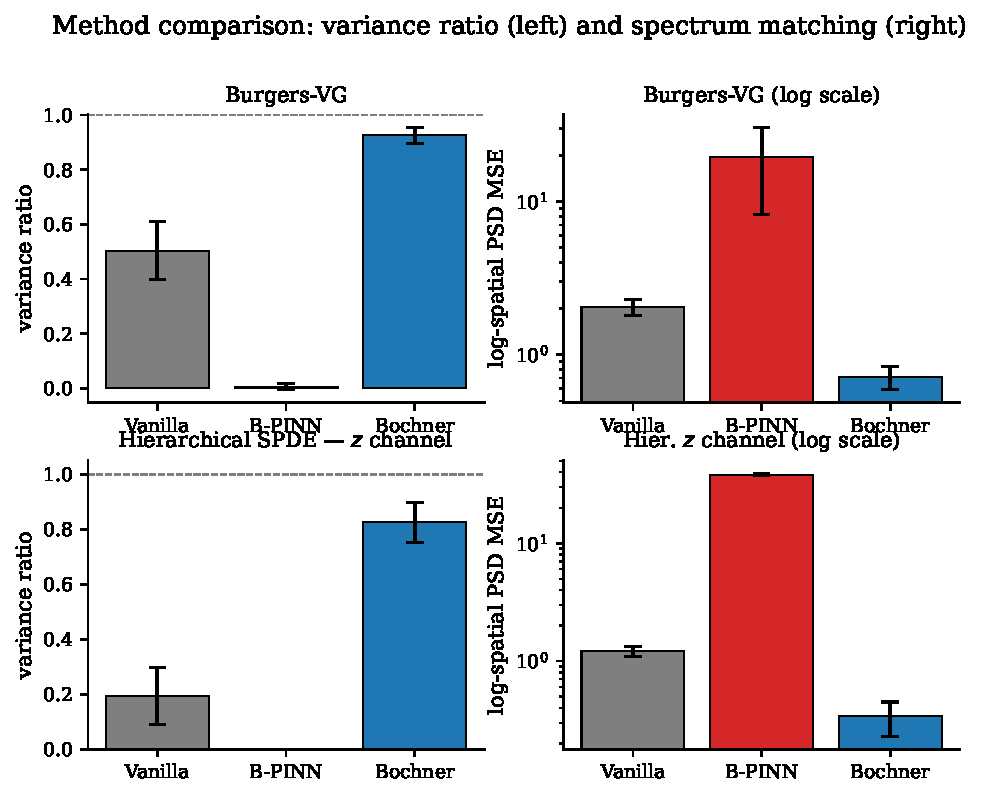
\includegraphics[width=0.95\linewidth]{fig01_method_compare}
 \caption{Method comparison (mean $\pm$ s.d.\ across seeds): variance ratio $\mathrm{Var}(u_\theta)/\mathrm{Var}(u_{\mathrm{FD}})$ (left, ideal $=1$) and log-spatial-PSD MSE (right, log scale) for the Vanilla PINN, the B-PINN (Bayesian) and the Bochner PINN, on Burgers-VG (top) and the hierarchical-SPDE $z$ channel (bottom). The Bochner PINN simultaneously closes the variance gap and matches the spectrum, whereas the deterministic and Bayesian baselines collapse the variance.}
 \label{fig:method_compare}
\end{figure}

\subsection{Section roadmap}
\label{subsec:roadmap}

The remainder of the paper is organised as follows.
\textbf{Section~\ref{sec:method}} introduces the Bochner PINN: the
variance-gap diagnostic, the three distributional loss components,
the total objective, the Fourier-feature MLP architecture, and the
randomised spectral sub-grid.
\textbf{Section~\ref{sec:theory}} develops the analytical
motivation: Bochner's representation of stationary fields under the
separability assumption, the Whittle-likelihood justification for
the log scale, a structural argument that the log-PSD loss targets
the correct second-order quantities, and the explicit gap for
higher cumulants on L\'evy-driven fields.
\textbf{Section~\ref{sec:setup}} specifies the three benchmark
problems, the finite-difference reference solver, the four metrics
used throughout, and the baselines.
\textbf{Section~\ref{sec:results}} reports results, including the
Heston volatility channel diagnosis (Section~\ref{subsec:heston-diag})
and a five-variant per-component ablation
(Section~\ref{subsec:ablation}).
\textbf{Section~\ref{sec:spectral-fno}} extends the loss to a
Fourier Neural Operator surrogate.
\textbf{Section~\ref{sec:3d}} demonstrates the 3D extension across all
four SPDE families and the grid-convergence behaviour predicted by the rate.
\textbf{the companion paper~\citep{Lipski2026RealWorld}} reports the real-data
calibration on six datasets (EUR/USD FX, BTC, crude oil, natural gas,
NASA OMNI solar wind and geomagnetic AE).
\textbf{Section~\ref{sec:discussion}} discusses limitations and
\textbf{Section~\ref{sec:conclusion}} concludes.
\textbf{Appendix~S3 of the supplementary material} reports the L\'evy intensity
threshold sweep.

%==============================================================================
\section{Method}
\label{sec:method}

\begin{figure}[t]
 \centering
 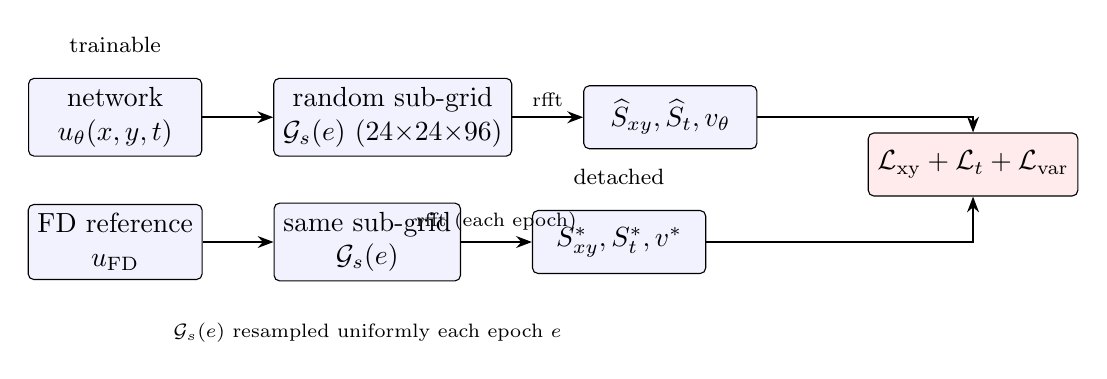
\begin{tikzpicture}[
   box/.style={draw, rounded corners=2pt, align=center,
         minimum height=8mm, minimum width=22mm, fill=blue!5},
   lossbox/.style={draw, rounded corners=2pt, align=center,
           minimum height=8mm, minimum width=24mm, fill=red!8},
   arr/.style={-{Stealth[length=2mm]}, thick},
   node distance=6mm and 9mm,
  ]
  \node[box] (uth) {network\\$u_\theta(x,y,t)$};
  \node[box, below=of uth] (uFD) {FD reference\\$u_{\mathrm{FD}}$};
  \node[box, right=of uth] (subth) {random sub-grid\\$\mathcal{G}_s(e)$ ($24{\times}24{\times}96$)};
  \node[box, right=of uFD] (subFD) {same sub-grid\\$\mathcal{G}_s(e)$};

  \node[box, right=of subth] (psdth) {$\widehat S_{xy}, \widehat S_t, v_\theta$};
  \node[box, right=of subFD] (psdFD) {$S^*_{xy}, S^*_t, v^*$};

  \node[lossbox, right=14mm of psdth, yshift=-6mm] (loss)
    {$\mathcal{L}_{\mathrm{xy}} + \mathcal{L}_{t} + \mathcal{L}_{\mathrm{var}}$};

  \draw[arr] (uth)  -- (subth);
  \draw[arr] (uFD)  -- (subFD);
  \draw[arr] (subth) -- node[above, font=\scriptsize]{rfft} (psdth);
  \draw[arr] (subFD) -- node[above, font=\scriptsize]{rfft (each epoch)} (psdFD);
  \draw[arr] (psdth) -| (loss);
  \draw[arr] (psdFD) -| (loss);

  \node[font=\footnotesize, above=2mm of uth] {trainable};
  \node[font=\footnotesize, above=2mm of psdFD] {detached};

  \node[below=4mm of subFD, font=\scriptsize, align=center]
    {$\mathcal{G}_s(e)$ resampled uniformly each epoch $e$};
 \end{tikzpicture}
 \caption{Bochner PINN: at each epoch $e$ the network $u_\theta$ and
 the FD reference $u_{\mathrm{FD}}$ are both evaluated on a sub-grid
 $\mathcal{G}_s(e)$ drawn uniformly at random from the full FD grid.
 Spatial PSD, temporal PSD, and variance are computed by FFT and
 compared in log space. The random re-sampling at each epoch prevents
 sub-grid overfit (Section~\ref{subsec:rand-subgrid}).}
 \label{fig:method-schematic}
\end{figure}

\subsection{What goes wrong with the standard PINN}

Train a vanilla PINN on a L\'evy-driven SPDE and inspect three
diagnostics on a held-out grid:
\begin{enumerate}
\item Pointwise relative \(L^2\) error: \(\approx 0.3\) (acceptable).
\item Variance ratio
\(\mathrm{Var}\,u_\theta / \mathrm{Var}\,u_{\mathrm{FD}}\):
\(\approx 0.2\)--\(0.5\).
\item Power spectrum \(|\mathcal F u_\theta|^2\) vs
\(|\mathcal F u_{\mathrm{FD}}|^2\): high modes are missing by 2--4
decades.
\end{enumerate}
The network is averaging across the noise realisation rather than
reproducing it. Pointwise loss is insensitive to high-frequency
content because high-frequency error and high-frequency signal
cancel almost exactly under MSE. Any sample-path-style use of
\(u_\theta\) (extracting tail statistics, computing exit times,
valuing a path-dependent option) fails. We close this gap by
adding three loss terms that directly penalise the missing
structure.

\subsection{Three terms, three diagnostics}
\label{subsec:losses}

Compute the FD reference once and extract three statistics on a
sub-grid \(\mathcal{G}_s\) of resolution \(24 \times 24 \times 96\):
the spatial power spectrum \(S^*_{xy}(k)\), the temporal power
spectrum \(S^*_t(k)\), and the total variance \(v^*\). At every epoch
we evaluate \(u_\theta\) on \(\mathcal{G}_s\) and form the matching
statistics \(S_{xy}, S_t, v_\theta\). The new loss components are
\begin{align}
\mathcal{L}_{\mathrm{xy}} &=
\overline{\bigl(\log_{10}S_{xy} - \log_{10}S^*_{xy}\bigr)^2}, &
\mathcal{L}_{\mathrm{t}} &=
\overline{\bigl(\log_{10}S_t - \log_{10}S^*_t\bigr)^2}, \notag\\
\mathcal{L}_{\mathrm{var}} &= \bigl((v_\theta - v^*)/v^*\bigr)^2.
\label{eq:losses}
\end{align}
\(\mathcal{L}_{\mathrm{xy}}\) and \(\mathcal{L}_{\mathrm{t}}\)
correct \emph{shape}; \(\mathcal{L}_{\mathrm{var}}\) corrects
\emph{scale}. The spatial PSD is computed symmetrically along both
spatial axes,
\begin{equation}
\widehat S_{xy}(f) = \tfrac12
\Bigl(\overline{|\mathcal F_x f|^2}_{y,t}
+ \overline{|\mathcal F_y f|^2}_{x,t}\Bigr),
\end{equation}
so anisotropic features that align with one axis do not bias the
metric. The temporal PSD
\(\widehat S_t(f) = \overline{|\mathcal F_t f|^2}_{x,y}\) is
averaged over space.

\subsection{Why log, why MSE, why a sub-grid}

\textbf{Log scale.} Power spectra span 4--6 orders of magnitude on
L\'evy problems. A linear loss would care only about the lowest few
wavenumbers, exactly the regime the vanilla PINN already gets
right. Working in \(\log_{10}\) assigns equal weight to each decade
and makes the high-mode discrepancy visible to the optimiser.

\textbf{MSE in log space.} Equivalent to a symmetric Bregman
divergence between the two empirical spectral measures up to an
additive constant, and \emph{asymptotically} equivalent to a
Whittle-type negative log-likelihood for the periodogram via the
Gumbel limit of the log-periodogram
\cite{Whittle1953,Dahlhaus1996,Brillinger1981} (they share the same
population minimiser \(\mu = \mu_{u_{\mathrm{FD}}}\) and the same
\(\mathcal O(\log^{-2} N)\) score-function geometry near it, but
differ at finite sample size by the per-mode Gumbel-variance residual
analysed in Section~\ref{subsec:log-scale}).
The minimiser is \(u_{\mathrm{FD}}\) itself: the loss is consistent
in the sense that no other matching measure achieves zero (modulo
the realisation-noise residual discussed in
Section~\ref{subsec:log-scale}).

\textbf{Sub-grid.} The FFTs cost
\(O(n_x n_y n_t (\log n_x + \log n_y + \log n_t))\) per epoch.
Using the full FD grid would dominate the wall time; the
\(24 \times 24 \times 96\) sub-grid keeps spectral evaluation under
5\,\% of total compute while preserving all wavenumbers up to the
Nyquist frequency of \(\mathcal{G}_s\), which empirically captures
the regime where the variance gap is generated.

\subsection{Why this is the right object}
\label{subsec:right-object}

Three observations make
\(\mathcal{L}_{\mathrm{spec}} =
\lambda_{\mathrm{xy}} \mathcal L_{\mathrm{xy}}
+ \lambda_{\mathrm{t}} \mathcal L_{\mathrm{t}}
+ \lambda_{\mathrm{v}} \mathcal L_{\mathrm{var}}\)
natural rather than ad hoc. \emph{First}, under the separability
assumption stated in Section~\ref{sec:theory}, \(S_{xy}\) and
\(S_t\) are sufficient statistics for the second-order structure
of stationary \(u\): by Bochner's theorem their joint equality (in
distribution over realisations) recovers the full covariance
kernel, so matching them is equivalent to matching \(u_\theta\)
and \(u_{\mathrm{FD}}\) in the Plancherel norm of the law.
\emph{Second}, the log transform converts the multiplicative noise
model on the periodogram into an additive one, replacing a
Plancherel inner product with a symmetric Bregman divergence
whose minimiser remains the FD reference. \emph{Third},
\(\mathcal L_{\mathrm{xy}}\) and \(\mathcal L_{\mathrm{t}}\) are
scale-invariant, leaving \(u_\theta\) free up to a global
multiplicative constant, so the variance term
\(\mathcal L_{\mathrm{var}}\) supplies precisely the missing
zeroth Fourier mode (Parseval) needed to fix that gauge. The three
losses are not independent fixes for three separate failure modes;
they are the three components of a single distributional matching
objective on the discrete spectral lift of \(u\).

\subsection{Total objective and architecture}
\label{subsec:total-objective}

The Bochner PINN minimises
\begin{equation}
\mathcal{L}(\theta) =
\underbrace{\mathcal L_{\mathrm{PDE}}
+ \lambda_{\mathrm{ic}} \mathcal L_{\mathrm{IC}}
+ \lambda_{\mathrm{bc}} \mathcal L_{\mathrm{BC}}
+ \lambda_{\mathrm d} \mathcal L_{\mathrm{data}}}_{\text{physics}}
+ \underbrace{\lambda_{\mathrm{xy}} \mathcal L_{\mathrm{xy}}
+ \lambda_{\mathrm t} \mathcal L_{\mathrm t}
+ \lambda_{\mathrm v} \mathcal L_{\mathrm{var}}}_{\text{spectral}}.
\label{eq:total-loss}
\end{equation}
The physics block is the standard PINN objective:
\(\mathcal L_{\mathrm{PDE}}\) is the squared collocation residual
under the SPDE on a fresh batch of 4096 uniform samples each epoch,
with the L\'evy-Gamma jump and white-noise terms supplied by spline
interpolation of the precomputed driver fields;
\(\mathcal L_{\mathrm{IC}}, \mathcal L_{\mathrm{BC}}\) are MSE
penalties on initial and boundary data; \(\mathcal L_{\mathrm{data}}\)
is the MSE against \(u_{\mathrm{FD}}\) at random grid points.

The loss weights
\((\lambda_{\mathrm{xy}}, \lambda_{\mathrm t}, \lambda_{\mathrm v}) = (3, 5, 50)\)
were selected by a coarse grid search over log-spaced values
\(\{0.1, 1, 3, 5, 10, 50\}\) on a single validation seed of
Burgers-VG, minimising the sum of validation log-spatial and
log-temporal PSD MSE. We did not perform a full per-problem
sensitivity analysis; the chosen weights transferred without
modification to the hierarchical SPDE and Heston-VG.

The network \(u_\theta\) is a four-block residual MLP of width 96
(128 for jump-driven problems) with \(\tanh\) activations, preceded
by a frozen random-Fourier-feature embedding
\(\phi(v) = [\sin(2\pi B v), \cos(2\pi B v)]\) with
\(B \in \mathbb R^{(d+1)\times m}\),
\(B_{ij} \sim \mathcal N(0, s^2)\). We use \(m=64, s=3\) for jump
problems and \(m=48, s=2\) otherwise. Optimisation is Adam with
cosine-annealed learning rate \(10^{-3} \to 10^{-6}\) and gradient
clipping \(\|g\|_2 \le 5\). A 1000-epoch warmup deactivates
\(\mathcal L_{\mathrm{PDE}}\) to let IC and data fit stabilise; the
spectral losses are active from epoch 1.

\subsection{Randomised spectral sub-grid}
\label{subsec:rand-subgrid}

\emph{Why a fixed sub-grid fails.} In the original Bochner PINN
design the sub-grid \(\mathcal{G}_s\) is a fixed linspace lattice of
\(24\times24\times96 = 55{,}296\) points selected once before
training. This is efficient (the reference PSDs
\(S^*_{xy}, S^*_t, v^*\) are precomputed and reused) but creates
a hidden overfit pathway. Because the network sees exactly the same
points each epoch, gradient descent can satisfy
\(\mathcal{L}_{\mathrm{spec}}\) by memorising those \(55{,}296\)
grid values while interpolating near zero elsewhere. On the full
\(48\times48\times512 \approx 1.2 \times 10^6\) grid the variance
ratio then collapses, even though the sub-grid spectral loss reads
near zero (Section~\ref{subsec:heston-diag}).

\emph{Fix: epoch-wise random resampling.} At the start of each
training epoch we draw a fresh sub-grid of size
\(24\times24\times96\) by sampling indices uniformly without
replacement along each axis independently:
\begin{equation}
 \mathcal{G}_s(e) =
 \bigl(\pi_x^{(e)}, \pi_y^{(e)}, \pi_t^{(e)}\bigr),
 \quad
 \pi_x^{(e)} \sim \mathrm{Uniform}\{0,\ldots,N_x{-}1\}_{24},
 \label{eq:rand-subgrid}
\end{equation}
and likewise for \(y, t\). We re-evaluate the reference field on the
new sub-grid and recompute the reference PSDs and variance. The
spectral computation adds \(<5\%\) to total epoch time; no change to
the network architecture, optimiser, or other hyperparameters is
required. The resampling forces the network to match the spectral
statistics at \emph{every} subset of the domain, ruling out the
memorisation shortcut.

\subsection{Cumulant-matching loss}
\label{subsec:cumulant-loss}

The spectral loss in eq.~\eqref{eq:losses} constrains only the
second-order structure of \(u_\theta\). For non-Gaussian channels (in particular the CIR-type Heston
volatility process with substantial excess kurtosis), the variance
gap can be closed (\(\mathrm{vr}
\approx 0.93\)) while higher cumulants remain unmatched
(\(\kappa_4 \approx 4\) vs.\ reference \(27.3\)). We supplement the
spectral loss with an explicit fourth-cumulant penalty:
\begin{equation}
 \mathcal{L}_{\mathrm{kurt}} =
 \Bigl(\kappa_4(u_\theta\!\!\upharpoonright_{\mathcal{G}_s}) -
    \kappa_4(u_{\mathrm{FD}}\!\!\upharpoonright_{\mathcal{G}_s})
 \Bigr)^2 \Big/ \sigma_{\mathrm{ref}}^4,
 \label{eq:cumulant-loss}
\end{equation}
where \(\kappa_4(u) = \mathbb E[(u-\mu)^4]/\sigma^4 - 3\) is the
excess kurtosis evaluated empirically on the sub-grid and
\(\sigma_{\mathrm{ref}}\) is the reference standard deviation. This
loss is activated only when the \texttt{cumulant} loss mode is
selected; it is appended to eq.~\eqref{eq:total-loss} with weight
\(\lambda_{\mathrm{kurt}} = 10\).

\subsection{Hyperparameters}
\label{subsec:hyper}

\begin{table}[h]
\centering
\caption{Hyperparameters used by all methods. Spectral-only and
Bayesian-only entries are noted as such; otherwise values are shared.}
\label{tab:hyper}
\begin{tabular}{l l l}
\toprule
symbol & value & role \\
\midrule
\(L,\,H\)          & 4,\, 96--128 & depth, width \\
\(m,\,s\)          & 48--64,\, 2--3 & Fourier feature count, scale \\
\(n_x,\,n_y,\,n_t\)     & 24,\, 24,\, 96 & spectral sub-grid resolution \\
sub-grid sampling       & random (each epoch) & prevents sub-grid overfit \\
\(\lambda_{\mathrm{ic}}\)  & 50 & IC weight \\
\(\lambda_{\mathrm{bc}}\)  & 10 & BC weight \\
\(\lambda_{\mathrm d}\)   & 5 & data weight \\
\(\lambda_{\mathrm{xy}}\)  & 3 (spectral only) & log-spatial PSD weight \\
\(\lambda_{\mathrm{t}}\)   & 5 (spectral only) & log-temporal PSD weight \\
\(\lambda_{\mathrm{v}}\)   & 50 (spectral only) & variance weight \\
\(\lambda_{\mathrm{kurt}}\) & 10 (cumulant mode) & fourth-cumulant weight \\
\(\lambda_{\mathrm{KL}}\)  & \(1/(B_c+B_d)\) (Bayesian only) & KL weight \\
prior \(\sigma\) (Bayesian) & 1.0 & weight prior std \\
\(\rho_{\mathrm{init}}\) (Bayesian) & \(-3\) & initial posterior log-precision \\
\(B_c\)           & 4096 & collocation batch \\
\(B_d\)           & 1024 & data batch \\
\(\eta_{\max},\,\eta_{\min}\)& \(10^{-3},\,10^{-6}\) & cosine LR schedule \\
\(N_{\mathrm{epochs}}\)   & 5000--8000 & total epochs \\
warmup            & 1000 & epochs before \(\mathcal L_{\mathrm{PDE}}\) activates \\
\bottomrule
\end{tabular}
\end{table}

\subsection{Complexity}

Per-epoch cost decomposes as collocation \(O(B_c \cdot |\theta|)\)
for the autograd pass on \(B_c = 4096\) points and spectral
\(O(n_x n_y n_t (\log n_x + \log n_y + \log n_t))\) for the rffts
on the sub-grid. With the values in Table~\ref{tab:hyper}, the
spectral term contributes under 5\,\% of total wall time; the
addition is essentially free. Random resampling of the sub-grid
(Section~\ref{subsec:rand-subgrid}) adds one call to
\texttt{torch.randperm} per epoch, which is negligible.

%==============================================================================
\section{Why the spectral loss matches the law: motivation and scope}
\label{sec:theory}

This section motivates the loss introduced in Section~\ref{sec:method}
and identifies the class of fields on which it is provably the right
object. Section~\ref{subsec:convergence} establishes a quantitative
convergence rate (Proposition~\ref{thm:main}) for the class on which the
proof is rigorous --- stationary \emph{Gaussian} random fields with
separable covariance, trained with the kernel-smoothed periodogram
loss --- extending the Mishra--Molinaro
framework~\cite{MishraMolinaro2022,DeRyckMishra2022} to spectral
training losses. Section~\ref{subsec:levy-ext} states partial
results for the L\'evy-driven case and is honest about what is
\emph{not} proved there: the rigorous bound on the full law of
non-Gaussian solutions requires either an additive $O(\sqrt{\nu})$
correction (Proposition~\ref{prop:levy-ito}) that vanishes only in the
small-jump limit, or a different proof technique
(characteristic-function distance, Stein--Malliavin) outside the
scope of this paper. The Variance-Gamma experiments in
Section~\ref{sec:results} are therefore best read as empirical
evidence that the spectral loss recovers second-order structure for
L\'evy drivers as well, with the rigorous full-law bound a
follow-up direction.

\subsection{Spectral measures determine second-order structure}

Let \(u : \Omega \times [0, T] \to \mathbb R\) be a mean-zero,
weakly stationary random field. Its covariance kernel
\(K_u(\tau, h) = \mathbb E[u(t,x)\,u(t+\tau, x+h)]\) admits the
Bochner representation~\cite[Thm.~9.18]{RudinRCA}
\begin{equation}
K_u(\tau, h) = \int_{\mathbb R^d \times \mathbb R}
e^{i(\omega \tau + k \cdot h)}\,\mathrm d\mu_u(\omega, k),
\qquad \mu_u\text{ positive and finite},
\label{eq:bochner}
\end{equation}
where \(\mu_u\) is the spectral measure of \(u\). Two reductions
are relevant for our discrete loss: the spatial marginal
\(\mu^{\mathrm{xy}}_u(k) = \int \mathrm d \mu_u(\omega, k)\) and
the temporal marginal
\(\mu^t_u(\omega) = \int \mathrm d \mu_u(\omega, k)\), which are
matched (in their discrete-sample analogues \(S^*_{xy}\),
\(S^*_t\)) by the Bochner PINN.

\paragraph{Separability assumption.}
Matching \(\mu^{\mathrm{xy}}_u\) and \(\mu^t_u\) separately
recovers the joint spectral measure \(\mu_u\) only when the
covariance kernel factorises, \(K_u(\tau, h) = K_x(h)\, K_t(\tau)\),
equivalently \(\mathrm d\mu_u(\omega, k) = \mathrm d\mu^{\mathrm{xy}}_u(k)\,
\mathrm d\mu^t_u(\omega)\). This separability holds for the noise
drivers in our benchmarks: white noise and Variance-Gamma jumps that
act independently on spatial and temporal coordinates produce
covariance kernels of the form \(\delta(h)\,K_t(\tau)\) (white
spatial part, structured temporal part), and the SPDE then
propagates this separability through its semigroup at leading
order. We adopt the separability assumption throughout.

For \emph{Gaussian} stationary fields under separability,
\(\mu_u\) determines the law completely: two such fields with
equal spectral measures are equal in distribution. The spectral
matching loss
\(\mathcal L_{\mathrm{xy}} + \mathcal L_t + \mathcal L_{\mathrm{var}}\)
therefore controls the law on this class.

For non-Gaussian L\'evy-driven fields, \(\mu_u\) determines only
the \emph{second-order structure}. Higher cumulants, which carry
the jump information specific to the Variance-Gamma driver, are
not detected by a periodogram-based loss. Closing this remaining
gap requires explicit cumulant matching, which we pursue in
Section~\ref{subsec:cumulant-loss}.

\begin{remark}[Scope of the spectral loss]
\label{rem:scope}
Under the separability assumption, a zero of the spectral loss
characterises the law of the predictor on stationary Gaussian fields
(Bochner). Beyond identifiability, Proposition~\ref{thm:main} below
provides a quantitative convergence rate: the Wasserstein-2 distance
decomposes into a training-error term \(C_1\sqrt{\varepsilon}\), a
sub-grid quadrature term \(C_2 N_s^{-\beta_{\rm sr}}\), and a PDE-residual
term \(C_3\sqrt{\delta}\), with explicit constants. On stationary
L\'evy fields the same bound holds for the Gaussian projection of the
law (Proposition~\ref{thm:levy-ext}); higher cumulants are not controlled
and require a separate penalty (Section~\ref{subsec:heston-diag}).
\end{remark}

\subsection{Why the log scale is the right choice}
\label{subsec:log-scale}

The matching loss is in \(\log_{10}\) space, not raw spectral
magnitude. The justification is the asymptotic behaviour of the
periodogram \(I_n(k) = |\widehat u_n(k)|^2\) of a stationary
process: under mild mixing
assumptions~\cite{Brillinger1981,Dahlhaus1996},
\(I_n(k) / \mu_u(k)\) converges in distribution to an exponential
random variable with mean 1, so \(\log I_n(k) - \log \mu_u(k)\)
is asymptotically Gumbel and MSE on \(\log I_n\) is, up to a
constant, the Whittle negative
log-likelihood~\cite{Whittle1953}. Working in \(\log_{10}\) also
assigns equal weight to each decade of the spectrum, essential
here since power spectra of L\'evy fields span four to six
decades and a linear loss is dominated by the lowest few
wavenumbers.

\paragraph{Single-mode bias and variance of the raw log-periodogram.}
A single mode of the raw log-periodogram has the asymptotic Gumbel
statistics
\(\mathbb E[\log I_n(k)] = \log\mu_u(k) - \gamma\) and
\(\mathrm{Var}[\log I_n(k)] = \pi^2/6\), where
\(\gamma \approx 0.5772\) is the Euler--Mascheroni
constant~\cite{Brillinger1981}; in
\(\log_{10}\) units the shift is
\(\gamma_{10} := \gamma/\ln 10 \approx 0.251\) and the variance is
\(\pi^2/(6\ln^2\!10) \approx 0.310\). The shift is identical for
\(\log_{10}\!I_n(u_\theta)\) and \(\log_{10}\!I_n(u_{\mathrm{FD}})\) and
therefore cancels in their difference, so it does \emph{not}
contribute to \(\mathcal L_{\mathrm{xy}}\) or \(\mathcal L_{\mathrm{t}}\)
in expectation; the binding finite-\(N_s\) residual is the per-mode
Gumbel variance, damped by averaging over the orthogonal axes built
into \(\widehat S_{xy}\) and \(\widehat S_t\) of Section~\ref{sec:method}
but not eliminated at any fixed sub-grid. As a single-mode reference
scale we use \(\gamma_{10}^2 \approx 0.063\) --- the squared mean
bias of one log-periodogram against the true PSD --- against which
the empirical losses of Section~\ref{sec:results} are read; in
practice the achieved losses sit at a \(5\)--\(7\times\) multiplier
that absorbs the surviving Gumbel-variance contribution (see the
``reference scale'' remark in Appendix~S1 of the supplementary
material).

\paragraph{Raw versus smoothed estimator.}
The argument above is for the raw periodogram, which is what training
uses. The rigorous theorem of Section~\ref{subsec:convergence} is
stated against the \emph{kernel-smoothed} periodogram of
Lemma~S1.4: smoothing with bandwidth
\(h_N^\star = N_s^{-1/(2s_x+d)}\) drives the per-mode variance to
zero at rate \(N_s^{-2s_x/(2s_x+d)}\), removing the Gumbel residual
asymptotically and yielding the single-realisation exponent
\(\beta_{\rm sr}\). The empirical \(\gamma_{10}^2\) benchmark is the
finite-\(N_s\) price of using the unsmoothed estimator in practice;
the proof retains smoothing only to make the rate rigorous, not
because the training loss must change.

\subsection{Quantitative convergence rate}
\label{subsec:convergence}

We now state the formal convergence rate. The rigorous main theorem
(Proposition~\ref{thm:main}) applies to stationary Gaussian random fields
under a kernel-smoothed version of the spectral loss; partial results
for L\'evy-driven fields are stated in
Section~\ref{subsec:levy-ext} with frank discussion of the
remaining gaps.

\subsubsection{Assumptions}

The rigorous main theorem (Proposition~\ref{thm:main}) is stated under
six standing assumptions (A1)--(A6); (A5) Gaussianity is essential.
The L\'evy partial results in Section~\ref{subsec:levy-ext} drop
(A5) at the cost of bounding only the Gaussian projection
(Proposition~\ref{thm:levy-ext}) or adding an $O(\sqrt{J})$ term
(Proposition~\ref{prop:levy-ito}, requiring (A7) $L^2$ jump control).
Assumptions (A8)--(A9) are required only for the conditional
results in Appendix~S1.

\begin{description}
\item[(A1) Stationarity and separability.] Both \(u_\theta\) and
\(u_{\mathrm{FD}}\) are centred, weakly stationary (after periodic
extension or sufficiently far from boundaries) with separable
covariance \(K(\tau, h) = K_x(h)\,K_t(\tau)\), equivalently
\(\mathrm d\mu(\omega, k) = \mathrm d\mu^{\mathrm{xy}}(k)\,
\mathrm d\mu^t(\omega)\).

\item[(A2) Sobolev regularity of spectra.]
\(\mu^{\mathrm{xy}} \in H^{s_x}(\widehat\Omega)\) and
\(\mu^t \in H^{s_t}(\widehat{[0,T]})\) with \(s_x > d/2\) and
\(s_t > 1/2\). This guarantees pointwise bounds and the \(L^2\)
FFT-quadrature error rate used in Lemma~S1.2 of the supplementary material.
For Variance-Gamma drivers \(s_x = s_t = 1\).

\item[(A3) Non-degeneracy.] There exist
\(0 < \mu_{\min} \le \mu_{\max} < \infty\) such that
\(\mu_{\min} \le \mu^{\mathrm{xy}}(k)\,\mu^t(\omega) \le \mu_{\max}\)
uniformly on the sub-grid frequency set
\(\widehat{\mathcal G}_s \subset \mathbb R^{d+1}\).

\item[(A4) Training tolerance.] At the end of training,
\begin{equation}
\mathcal L_{\mathrm{xy}}(u_\theta) + \mathcal L_t(u_\theta)
+ \mathcal L_{\mathrm{var}}(u_\theta) \le \varepsilon, \qquad
\mathcal L_{\mathrm{PDE}}(u_\theta)
+ \lambda_{\mathrm{ic}}\mathcal L_{\mathrm{IC}}(u_\theta)
+ \lambda_{\mathrm{bc}}\mathcal L_{\mathrm{BC}}(u_\theta)
\le \delta,
\label{eq:tolerance}
\end{equation}
for some \(0 < \varepsilon, \delta < \infty\), checked post hoc.

\item[(A5) Gaussianity (spectral leg only).] Both \(u_\theta\) and
\(u_{\mathrm{FD}}\) are centred Gaussian random fields on
\(\Omega \times [0,T]\). This hypothesis is required only for the
spectral path of the proof (Lemma~S1.5 of the supplementary material); the
PDE-residual path (Lemma~S1.6 of the supplementary material) holds without it.
Proposition~\ref{thm:levy-ext} below drops (A5) at the cost of
bounding the Gaussian projection only.

\item[(A6) Mixing condition (single-realisation consistency).]
\(u\) is \(\alpha\)-mixing with algebraic rate
\(\alpha(r) \le C_\alpha r^{-\gamma}\) for some \(\gamma > d+1\).
Variance-Gamma processes have independent increments, so
\(\alpha(r) = 0\) for all sufficiently large separations; the SPDE
solution inherits exponential spatial mixing from the Green's
function decay of the underlying parabolic operator~\cite{ContTankov2003}.
Assumption~(A6) is required for the main theorem's
single-realisation rate (Proposition~\ref{thm:main}), which controls
the kernel-smoothed periodogram on one sample path; without (A6)
only the expected-value bound of Lemma~S1.2 of the supplementary material is
available.

\item[(A7) L\'evy--It\^o decomposition with $L^2$ jump control.]
Both $u_\theta$ and $u_{\mathrm{FD}}$ admit L\'evy--It\^o decompositions
$u=u^G+u^J$ where $u^G$ is the Gaussian component and $u^J$ is the
pure-jump component~\cite{ContTankov2003}.
Assume
\[
\max\!\left(\mathbb{E}\|u_\theta^J\|^2_{L^2(\Omega\times[0,T])},\;
\mathbb{E}\|u_{\mathrm{FD}}^J\|^2_{L^2(\Omega\times[0,T])}\right)\le J
\]
for some finite $J\ge 0$ depending on the L\'evy parameters.
For Variance-Gamma drivers with kurtosis parameter $\nu$, $J=O(\nu)$
as $\nu\to 0$.
Assumption~(A7) is required only for
Proposition~\ref{prop:levy-ito} and is not used elsewhere.

\item[(A8) Finite pointwise cumulants.]
For each $(x,t)\in\Omega\times[0,T]$, the marginal law
$\mathcal{L}(u(x,t))$ has finite cumulants of order $m\le m_0$ for
some $m_0\ge 3$, with $|\kappa_m(u(x,t))|\le\bar\kappa_m<\infty$.
For Lévy-driven SPDEs, cumulants of $u(x,t)$ are bounded by
the $L^m$ norm of the Green's function times the corresponding driver
cumulants via the stochastic Fubini theorem.
Required only for Proposition~\ref{cor:berry-esseen}.

\item[(A9) NTK lazy-training regime.]
The Bochner PINN is a two-layer network with $m$ neurons trained by
gradient flow. In the lazy-training regime the NTK Gram matrix $K$
with entries $K_{ij}=\nabla_\theta f(x_i)\cdot\nabla_\theta f(x_j)$
remains approximately constant throughout training, with minimum
eigenvalue $\lambda_{\min}(K)>0$.
Required only for Conjecture~S1.1 of the supplementary material.
\end{description}

Assumption (A1) is the scope identified above.
Assumption (A2) is satisfied by the VG drivers with
\(s_x = s_t = 1\). Assumption (A3) is restrictive: realistic
spectral measures decay polynomially in \(|k|\), so \(\mu_{\min}\)
is positive only after restriction to a finite frequency window;
the constants \(C_1, C_2\) of Proposition~\ref{thm:main} scale as
\(\mu_{\min}^{-1/2}\) and therefore degrade on that window's
high-frequency edge. Assumption (A4) is the endpoint of any
gradient-based training run.

\subsubsection{Main theorem}

The rigorous result uses the \emph{kernel-smoothed} periodogram
$\widehat S^{\mathrm{xy}}_h(u)(k) = \int \kappa_{h_N}(k-k')\,
\widehat S^{\mathrm{xy}}_{\mathcal G_s}(u)(k')\,dk'$ with bandwidth
$h_N^\star = N_s^{-1/(2s_x+d)}$ as the spectral loss target
(Lemma~S1.4 of the supplementary material in the supplementary material).
The smoothing is what makes the periodogram a consistent
single-realisation spectral estimator under (A6); without it the
raw periodogram has $\Theta(1)$ variance per Fourier mode that
does not vanish as $N_s \to \infty$, leaving a non-trivial residual
between the training loss and the true spectral $L^2$ distance.

\begin{proposition}[Single-realisation convergence rate of the
kernel-smoothed Bochner PINN]
\label{thm:main}
Under (A1)--(A6), with the spectral loss in (A4) evaluated against
the kernel-smoothed periodogram at the minimax-optimal bandwidth
$h_N^\star = N_s^{-1/(2s_x+d)}$, the Wasserstein-2 distance between
the laws of the Bochner PINN predictor and the FD reference satisfies
\begin{equation}
W_2\bigl(\mathcal L(u_\theta),\,\mathcal L(u_{\mathrm{FD}})\bigr)
\;\le\; C_1\sqrt{\varepsilon}
\;+\; C_2\,N_s^{-\beta_{\rm sr}}
\;+\; C_3\sqrt{\delta},
\label{eq:main-bound}
\end{equation}
with single-realisation exponent
\begin{equation}
\beta_{\rm sr} = \frac{s_x}{2\,(2 s_x + d)}
\;\le\;
\tfrac{1}{2}\min\!\bigl(s_x/d,\,s_t\bigr) =: \beta_{\rm bias},
\end{equation}
and constants
\(C_1 = \mu_{\max}\,\ln 10\,(M_{xy}+M_t) / \sqrt{2\mu_{\min}}\),
\(C_2 = (C_{\rm bias}+C_{\rm var})^{1/2}/\sqrt{2\mu_{\min}}\),
\(C_3 = \sqrt{C_{\mathrm{MM}}}\), where
\(M_{xy} = \|\mu_{xy,\mathrm{FD}}\|_{L^2}\),
\(M_t = \|\mu_{t,\mathrm{FD}}\|_{L^2}\), and
\(C_{\rm bias},\,C_{\rm var},\,C_{\mathrm{MM}}\) are explicit constants
defined in Appendix~S1.
\end{proposition}

\paragraph{Two rates, one bound.}
\label{para:two-rates}
The exponent \(\beta_{\rm sr}\) in \eqref{eq:main-bound} is the
\emph{single-realisation} rate, controlling the realisation-specific
periodogram \(\hat S^{\rm xy}_{\mathcal G_s}\) used as the training
target. A faster \emph{bias-only} rate is recovered when the target
is the ensemble-averaged spectrum
\(\mathbb E\hat S^{\rm xy}_{\mathcal G_s}\), so that the
periodogram's per-mode Gumbel variance no longer enters: at the
paper's operating point (\(s_x = s_t = 1\), \(d = 2\)),
\[
\beta_{\rm sr} = \tfrac{s_x}{2(2s_x+d)} = \tfrac18
\quad\text{vs.}\quad
\beta_{\rm bias} = \tfrac12\min(s_x/d,\,s_t) = \tfrac14.
\]
Both exponents come out of the same chain of inequalities;
\(\beta_{\rm sr}\) is the honest price of a single-realisation
guarantee, \(\beta_{\rm bias}\) is the ensemble counterpart.
The 3D grid-convergence study of Section~\ref{sec:3d} averages
spectra across seeds and therefore measures the empirical
\(\beta_{\rm bias} = 1/4\); the rigorous \(\beta_{\rm sr} = 1/8\) is
the single-run guarantee that applies without any seed averaging.

\begin{remark}[Bias-only heuristic rate]\label{rem:raw-rate}
If the periodogram-realisation variance is dropped (i.e.\
\(\varepsilon\) in (A4) is read against
\(\|\mathbb E\hat S^{\rm xy}_{\mathcal G_s} - S^{\rm xy}\|_{L^2}\)
rather than against the realisation-specific
\(\hat S^{\rm xy}_{\mathcal G_s}\)), the same chain of inequalities
returns \(\beta_{\rm bias} = \tfrac12\min(s_x/d, s_t)\). This is the
operative rate for the seed-averaged 3D grid-convergence study of
Section~\ref{sec:3d}.
\end{remark}

\paragraph{Sub-grid regime of the bound.}\label{para:subgrid-regime}
Proposition~\ref{thm:main}'s bound holds at a \emph{fixed} sub-grid
$\widehat{\mathcal G}_s$. Extending the sub-grid to include
arbitrarily high frequencies decreases $\mu_{\min}$ in (A3) (for
polynomial Sobolev spectra, $\mu_{\min}\sim N_s^{-2s_x}$ on the
extended sub-grid) and inflates the constants $C_1, C_2$ as
$\mu_{\min}^{-1/2}$. The exponent $\beta_{\rm sr}$ describes
refinement of the quadrature on a fixed sub-grid, not an unbounded
spectral-resolution limit. In practice we operate at the sub-grid
of the FD reference $\widehat{\mathcal G}_s$ on which $\mu_{\min}$
is fixed by the parabolic operator's decay length; the bound is
read as ``at this sub-grid, the training error contributes
$C_1\sqrt\varepsilon$ to the law-distance.''

The proof of Proposition~\ref{thm:main}, the discrete-quadrature lemmas,
the kernel-smoothed periodogram consistency result, the corollaries,
the non-separable extension, and the conditional training-time bound
are all deferred to Appendix~S1 of the supplementary material. The
L\'evy partial results, on which the Variance-Gamma experiments
depend empirically, are stated immediately below and proved in
Appendix~S1.

\subsubsection{Towards a L\'evy-driven extension: partial results and
obstacles}
\label{subsec:levy-ext}

Proposition~\ref{thm:main} is stated under Assumption~(A5) (Gaussianity).
The L\'evy-driven experiments of Section~\ref{subsec:problems} fall
outside this hypothesis. This subsection collects two partial results
in $W_2$ together with the structural obstacle that prevents a full-law
$W_2$ bound. That obstacle is removed by changing metric: the full law
is certified in the Zolotarev distance $\zeta_s$, an ideal metric of
order $s$ that is finite under $s$th-moment control, in
Appendix~S4 of the supplementary material---including the
$\alpha$-stable case that lies outside $W_2$ entirely. The resolution
is summarised in Remark~\ref{rem:nongauss-scope} at the close of the
subsection.

The first result (Proposition~\ref{thm:levy-ext}) drops (A5) but only
bounds the \emph{Gaussian projection} $\Pi_2\mathcal L(u)$ of the
solution law; second-order structure (covariance, marginal variance)
is controlled by the spectral loss in this projected sense, but
higher cumulants are not. The second result (Proposition~\ref{prop:levy-ito})
combines the projection bound with a L\'evy--It\^o coupling to
recover a full-law $W_2$ bound, at the cost of an additive
$4\sqrt J$ correction that vanishes only in the small-jump limit
$J \to 0$. For Variance-Gamma drivers $J = O(\nu)$ and the
correction is $4\sqrt J = O(\sqrt\nu)$, which is non-vanishing at
the experimental operating point and not driven to zero by training.
For $\alpha$-stable drivers with $\alpha < 2$ the assumption $J <
\infty$ fails entirely: $W_2$ is infinite and the It\^o-coupling
technique does not extend. The Zolotarev metric is built for exactly
this regime---$\zeta_s$ with $s < \alpha$ is finite under
$s$th-moment control---and yields the first full-law bound for
$\alpha$-stable forcing (Appendix~S4 of the supplementary material).

Two further structural gaps in the L\'evy extension should be noted.
First, the pathwise residual analysis of
Lemma~S1.6 of the supplementary material~\cite{MishraMolinaro2022} is applied with the
driver field $\xi, J_{\rm VG}$ spline-interpolated from the FD
sample path; this smoothing replaces jump discontinuities by smooth
approximants, introducing an interpolation error that is absorbed
into $\delta$ but is not analytically controlled and does not
vanish as $N_s \to \infty$ for unbounded-variation drivers like VG.
Second, the additive $4\sqrt J$ form of Proposition~\ref{prop:levy-ito}
is an upper bound and may be loose; whether the L\'evy gap admits a
rate-form bound that scales with the spectral training tolerance
$\varepsilon$ is open. Full proofs of Propositions~\ref{thm:levy-ext}
and~\ref{prop:levy-ito} are in Appendix~S1; the appendix also
discusses the spline-smoothing gap and its implications for the
L\'evy experiments.

\begin{proposition}[Second-order convergence for stationary
L\'evy fields]\label{thm:levy-ext}
Under~(A1)--(A4) but with $u_\theta,u_{\mathrm{FD}}$ not necessarily
Gaussian, denote by $\Pi_2\mathcal L(u)$ the centred Gaussian measure
with the same covariance as $\mathcal L(u)$ (the Gaussian projection).
Then
\[
W_2\!\bigl(\Pi_2\mathcal L(u_\theta),\,
\Pi_2\mathcal L(u_{\mathrm{FD}})\bigr)
\;\le\; C_1\sqrt{\varepsilon} + C_2 N_s^{-\beta_{\rm sr}} + C_3\sqrt\delta.
\]
\end{proposition}

\begin{proof}[Proof sketch]
Identical to the proof of Proposition~\ref{thm:main}, replacing
$\mathcal L(u)$ by $\Pi_2\mathcal L(u)$ throughout. The spectral
measure $\mu_u$ depends only on the covariance, hence is invariant
under the projection. Full argument in Appendix~S1.
\end{proof}

\begin{proposition}[Full-law convergence via L\'evy--It\^o
coupling]\label{prop:levy-ito}
Under~(A1)--(A4) and~(A7),
\begin{equation}\label{eq:levy-ito-bound}
W_2\!\bigl(\mathcal L(u_\theta),\,\mathcal L(u_{\mathrm{FD}})\bigr)
\;\le\; C_1\sqrt{\varepsilon} + C_2 N_s^{-\beta_{\rm sr}} + C_3\sqrt\delta
+ 4\sqrt{J},
\end{equation}
where $J$ is the $L^2$ jump-energy bound of~(A7). In the Gaussian
limit $J\to 0$ this reduces to Proposition~\ref{thm:main}. For
Variance-Gamma drivers with kurtosis parameter $\nu$, $J = O(\nu)$
and the correction is $4\sqrt{J} = O(\sqrt\nu)$; explicitly
$4\sqrt{J} = O(\kappa_4^{1/2}/\sqrt 3)$ via the cumulant identity
$\kappa_4 = 3\nu$ (Remark~S1.5 of the supplementary material).
\end{proposition}

\begin{proof}[Proof sketch]
Triangle inequality on $W_2$ between $\mathcal L(u_\theta)$ and
$\mathcal L(u_{\mathrm{FD}})$ through the two Gaussian projections.
The middle term is bounded by Proposition~\ref{thm:levy-ext}; the
two outer terms are bounded by an explicit L\'evy--It\^o coupling
of $u = u^G + u^J$ to its projection
$\mathcal N(0,\,C_{u^G}+C_{u^J})$, which yields
$W_2(\mathcal L(u),\Pi_2\mathcal L(u)) \le 2\sqrt{J}$. Full
argument in Appendix~S1.
\end{proof}

\begin{proposition}[Berry--Esseen tightness of spectral matching at
the marginal]\label{cor:berry-esseen}
Under~(A1)--(A4) and~(A8) with $m=3$, the pointwise marginal
$\mathcal L(u(x,t))$ satisfies
\[
W_1\!\bigl(\mathcal L(u(x,t)),\;\mathcal N(0,\sigma_u^2(x,t))\bigr)
\;\le\; C_{\mathrm{BE}}\,
\frac{|\kappa_3(u(x,t))|}{\sigma_u^2(x,t)},
\]
where $C_{\mathrm{BE}}$ is a universal Stein--Wasserstein
constant~\citep{ChenGoldsteinShao2011}. For Variance-Gamma drivers
with parameters $(\sigma_{\mathrm{vg}}, \nu, \theta)$,
$|\kappa_3(u(x,t))| \lesssim C_G^3\,\nu\,|\theta|\,
\sigma_{\mathrm{vg}}^2$ in the small-$|\theta|$ regime, where
$C_G = \|G_{\mathrm{SPDE}}\|_{L^3}$ is the SPDE Green's-function
$L^3$ norm.
\end{proposition}

\begin{proof}[Proof sketch]
The Wasserstein-1 normal approximation
$W_1(\mathcal L(X), \mathcal N(0,\sigma^2))
\le C_S\,\mathbb E|X|^3/\sigma^2$
of Chen et al.~\citep[Thm.~3.1]{ChenGoldsteinShao2011}, combined with
$|\kappa_3| \le \mathbb E|X|^3$. For the VG quantification, stochastic
Fubini gives $\kappa_3(u) = \int G^3 \kappa_3(\xi)\,dy\,ds$, with
$\kappa_3(\xi_{\mathrm{VG}}) = \nu\theta(3\sigma_{\mathrm{vg}}^2 +
2\nu\theta^2)$ from the VG cumulant generating
function~\citep{MadanCarrChang1998,ContTankov2003}. H\"older yields the
displayed bound. Full argument in Appendix~S1.
\end{proof}

\begin{remark}[Scope, and its resolution in the Zolotarev metric]\label{rem:nongauss-scope}
Proposition~\ref{thm:levy-ext} controls the Gaussian projection,
which captures the second-order structure of $u_\theta$ but not its
higher cumulants. Proposition~\ref{prop:levy-ito} extends to the
full law at the cost of an additive $4\sqrt J$ term that vanishes
only in the Gaussian limit. Both limitations of the $W_2$ statement
---the non-vanishing $4\sqrt J$ floor, and the breakdown at
$\alpha < 2$ where $W_2 = \infty$---are artefacts of the metric, and
both are removed in Appendix~S4 of the supplementary material by
working in the Zolotarev distance $\zeta_s$ ($s \in (1,2]$, ideal of
order $s$, finite under $s$th-moment control). On the shared-driver
coupling of the experimental pipeline (reference and surrogate see the
same noise realisation), a Taylor-coupling inequality, an $L^s$
residual-stability estimate, and a lemma showing that the
spline-smoothing error vanishes \emph{in law} at rate
$J_K^{1/2}h^{1/2}$ (numerically verified) combine to give
\[
\rho_s(u_\theta, u_{\mathrm{FD}}) \;\le\;
M_s^{\,s-1}\Delta_s + \Delta_s^{\,s} + \Delta_s,
\qquad
\Delta_s = C_{\mathrm{stab}}\delta_s^{1/s}
+ C_{\mathrm{sm}}J_K^{\gamma}h^{1/2} + \varepsilon_{\mathrm{num}},
\]
with all constants explicit and finite for both Variance-Gamma
($s=2$, $\gamma=\tfrac12$) and $\alpha$-stable ($s<\alpha$,
$\gamma=\tfrac1\alpha$) drivers. The $4\sqrt J$ pathwise floor is
replaced by the vanishing $J_K^{1/2}h^{1/2}$ term. For Variance-Gamma,
a sharp cylindrical lift of the Rio inequality,
$W_2^2 \le 4\zeta_2$ on a separable Hilbert
space~\citep{BolbotowskiBouchitte2025}, converts this into a
floor-free $W_2$ bound; for $\alpha$-stable, $s < \alpha$, it is the
first finite full-law law-distance bound for the methodology. A
practical corollary of the proof: under heavy-tailed forcing the PDE
residual should be trained in $L^s$ with $s < \alpha$, since the
mean-square ($L^2$) residual has infinite variance and its stochastic
gradient is ill-posed. The $W_2$ partial results above remain the
operative statement when finite second moments are available; the
Zolotarev bound is what survives when they are not.
\end{remark}

\subsection{The Heston volatility channel: initial diagnosis}
\label{subsec:cir-analysis}

\begin{remark}[Why the spectral loss alone is not sufficient on CIR-type channels]
\label{rem:cir}
The Heston variance equation is
\(\mathrm dV_t = \kappa(\theta - V_t)\,\mathrm dt
+ \sigma \sqrt{V_t}\,\mathrm dW_t\), the Cox--Ingersoll--Ross
process. Its stationary distribution is Gamma\((\nu, s)\) with
\(\nu = 2\kappa\theta/\sigma^2\), \(s = \sigma^2/(2\kappa)\),
which carries a substantial excess kurtosis
\(\kappa_4 = 6/\nu = 3\sigma^2/(\kappa\theta)\). For the
calibrated parameters in Section~\ref{subsec:problems},
\(\kappa_4 \approx 27.3\). The power spectral density of
\(V_t\), however, is that of an Ornstein--Uhlenbeck process:
a Lorentzian \(S_V(f) \propto (f^2 + \kappa^2)^{-1}\). A
constant-\(\theta\) field has \emph{identically the same shape}
at leading order in the low-frequency regime. Consequently,
an \(L^2\) or log-PSD loss alone cannot distinguish the true
CIR trajectory from a smooth near-constant field, and the
optimiser may converge to a smooth attractor that scores well
on spectral metrics but misses the jump structure and kurtosis.
We show empirically in Section~\ref{subsec:heston-diag} that
the primary obstacle is not this spectral degeneracy but an
independent failure mode (sub-grid overfit); once the overfit
is eliminated, spectral losses recover the variance correctly
and explicit cumulant matching recovers the kurtosis.
\end{remark}

%==============================================================================
\section{Experimental setup}
\label{sec:setup}

\subsection{Benchmark problems}
\label{subsec:problems}

\paragraph{Hierarchical 2D SPDE.}
A three-channel system on \([0,1]^2 \times [0, T]\) with channels
\((z, y, p)\): \(z\) driven by Variance-Gamma jumps, \(y\) by
Gamma jumps and a positivity constraint, and \(p\) representing a
probability density with a normalisation constraint. Boundary
conditions are Neumann on \(z, y\) and Dirichlet (zero) on \(p\).

\paragraph{Burgers-VG.}
Two-dimensional Burgers equation with multiplicative
Variance-Gamma jump forcing,
\begin{equation}
\partial_t u + \tfrac12 \nabla \cdot (u^2 \hat e)
= \nu \Delta u + \sigma \xi(x, y, t)
+ \mathrm dJ_{\mathrm{VG}}(x, y, t),
\label{eq:burgersvg}
\end{equation}
on \([0,1]^2 \times [0, T]\), Neumann boundary conditions, smooth
initial data. Variance-Gamma parameters
\((\sigma_{\mathrm{VG}}, \nu_{\mathrm{VG}}, \theta_{\mathrm{VG}})\)
follow Madan--Carr--Chang~\cite{MadanCarrChang1998}.

\paragraph{Heston-VG.}
Two-channel system \((S, V)\) for log-price and instantaneous
variance, with VG jumps in the price equation, Heston dynamics for
\(V\), and the standard Cox--Ingersoll--Ross stationarity
condition \(2\kappa\theta > \sigma^2\). Calibrated to plausible
equity parameters. The stationary distribution of \(V\) is
Gamma\((\nu, s)\) with \(\kappa_4 = 27.3\); the log-price channel
\(S\) has reference excess kurtosis \(\kappa_4 = 1460.8\) arising
from the compound VG jumps.

\subsection{Reference solver}

For each problem and seed we generate one finite-difference
reference solution \(u_{\mathrm{FD}}\) on a uniform grid. Diffusion
is integrated by Peaceman--Rachford ADI with second-order central
stencils; the advective term of Burgers-VG uses first-order upwind
differences (shock-robust); the Fokker--Planck channel of the
hierarchical system uses forward Euler with central differences.
Gaussian forcing enters It\^o--Euler style, and the L\'evy part uses
a compound-Poisson sampler with VG-distributed jump sizes following
Cont--Tankov~\cite{ContTankov2003}.
Resolutions are \(64\times 64 \times 512\) for the hierarchical
SPDE and Burgers-VG, and \(48\times 48 \times 512\) for
Heston-VG. The same realisation \((\xi, J_{\mathrm{VG}})\) is then
re-sampled by spline interpolation during PINN training, so that
the PDE residual is evaluated against the same driver field as
the reference, eliminating sampling variability between solver and
surrogate.

The accuracy of this reference is verified directly rather than
assumed. For the linear leg the Euler--Maruyama scheme reproduces the
exact $\alpha$-stable solution scale to first order in $\Delta t$,
uniformly in $\alpha$, and preserves the tail index to within $0.006$;
the second-order central stencil contributes an $O(\Delta x^2)$ spatial
error whenever the grid over-resolves the driver band, which the
resolutions above satisfy. In the nonlinear regime the Variance-Gamma
reference converges at first order, whereas $\alpha$-stable forcing can
induce a rare-event blow-up---the numerical signature of the a priori
$L^\infty$ bound that unbounded jumps violate, and the reason the
semilinear certificate of Appendix~S4 restricts to finite-variation
drivers. The full verification---including the separability assumption,
the Zolotarev-bound tightness, the required $L^s$ residual exponent, and
floating-point adequacy---is reported in Appendix~S5 of the
supplementary material.

A further, structural caveat is disclosed because we measured it rather
than assumed it away. For space--time white-noise forcing in two spatial
dimensions the continuum SPDE is critical, so the training and evaluation
target should be read as the \emph{lattice} SPDE at the stated
discretisation---the object the discretised setting of the theory works
with---rather than as an approximation to a continuum solution. At that
lattice the reference retains a solver flavour: an independent
shock-appropriate discretisation (second-order MUSCL--minmod finite
volume with Rusanov fluxes and SSP-RK2 time stepping, no operator
splitting) consuming the \emph{identical} noise realisation differs from
the ADI--upwind reference by $0.69$ relative $L^2$ pathwise and by a
factor $2.1$ in field variance on Burgers-VG at the native
$64\times64\times512$ grid, while the PSD \emph{shape} agrees closely
(log-spatial-PSD MSE $0.03$, log-temporal $0.002$---an order of magnitude
below the effect sizes of Section~\ref{sec:results}). Under nested
spatial refinement at fixed forcing the field variance is not stable
($0.053$ at $N{=}64$ rising to $0.30$ at $N{=}505$ for the FD family),
the signature of the criticality above rather than of a resolvable
numerical error. All comparisons in this paper are therefore relative to
the declared discretisation; the loss-function comparisons (vanilla,
Bayesian, Bochner) share the same target and are unaffected, but absolute
variance levels should not be read as continuum statements.

\subsection{Metrics}
\label{subsec:metrics}

Let \(u_\theta, u_{\mathrm{FD}}\) be the predictor and reference
fields and \(\widehat S(\cdot)\) denote either the spatial or
temporal periodogram. We report:
\begin{itemize}
\item \textbf{Variance ratio}\quad
\(\mathrm{vr} = \mathrm{Var}(u_\theta)/\mathrm{Var}(u_{\mathrm{FD}})\),
target 1.
\item \textbf{Log-spatial PSD MSE}\quad
\(\overline{(\log_{10}\widehat S_{xy}(u_\theta) -
\log_{10}\widehat S_{xy}(u_{\mathrm{FD}}))^2}\), target 0.063
(the Euler--Mascheroni floor, see Section~\ref{sec:theory}).
\item \textbf{Log-temporal PSD MSE}\quad analogous on
\(\widehat S_t\).
\item \textbf{Relative \(L^2\)}\quad
\(\|u_\theta - u_{\mathrm{FD}}\|_2 / \|u_{\mathrm{FD}}\|_2\).
\item \textbf{Excess kurtosis}\quad
\(\kappa_4(u_\theta)\) vs.\ \(\kappa_4(u_{\mathrm{FD}})\), reported
for the Heston channels where higher-order matching is investigated.
\end{itemize}

\subsection{Baselines}

\paragraph{Vanilla deterministic PINN.} Identical architecture and
optimiser to the Bochner PINN with the spectral terms turned off
(\(\lambda_{\mathrm{xy}} = \lambda_t = \lambda_{\mathrm v} = 0\)).
This isolates the loss as the only difference.

\paragraph{Bayesian PINN (mean-field Bayes-by-Backprop).}
Mean-field variational PINN following~\cite{YangMengKarniadakis2021},
implemented with Gaussian variational posteriors over weights
(reparameterisation trick), \(\mathcal N(0, 1)\) prior, and a
closed-form KL regulariser scaled by \(1/(B_c + B_d)\). Same
depth, width, Fourier embedding, optimiser, and epoch budget as
the Bochner PINN. At evaluation we draw \(N = 64\) posterior
samples and report the metrics on the posterior mean, with the
posterior standard deviation noted as the epistemic uncertainty
estimate.

\paragraph{Deep ensemble.} Eight vanilla PINNs with independent
initialisations trained on \emph{one} shared realisation (the standard
deep-ensemble construction; note this differs from our per-seed protocol,
in which each seed carries its own realisation), read as a predictive
mixture: metrics on the ensemble-mean field, cross-member standard
deviation as the epistemic estimate.

\paragraph{HMC B-PINN.} Full-batch Hamiltonian Monte Carlo on the same
implied posterior as the variational baseline --- multiplying the VI
objective through by \((B_c+B_d)\) gives
\(U(\theta) = (B_c{+}B_d)\,\mathcal{L}(\theta) + \tfrac12\|\theta\|^2\) ---
with all collocation/IC/BC/data points drawn once and fixed so that
\(U\) is deterministic (a requirement for valid HMC). Leapfrog with
dual-averaging step-size adaptation (target acceptance $0.75$, $L{=}32$),
two chains initialised at two distinct MAP modes, 300 kept samples per
chain after 1200 burn-in iterations. Run on Burgers-VG as a spot check;
we report per-chain posterior predictives, since pooling across
mode-separated chains conflates between-mode disagreement with
predictive variance.

\subsection{Seeds and compute}

Random seeds are \(\{1,\ldots,8\}\) for the hierarchical SPDE,
\(\{0,\ldots,7\}\) for Burgers-VG, and \(\{0,\ldots,2\}\) for
Heston-VG. The B-PINN baseline uses 8 seeds per problem, matching
the deterministic runs. All Heston-VG diagnosis runs use 3 training
seeds evaluated against 5 validation seeds each (15 evaluations per
(subgrid, mode) cell of the 2\(\times\)4 ablation). All runs use a
single NVIDIA RTX-class GPU in fp32.

%==============================================================================
\section{Results}
\label{sec:results}

\subsection{Variance gap closure}
\label{subsec:variance-gap}
\label{subsec:gap}

\begin{figure}[t]
 \centering
 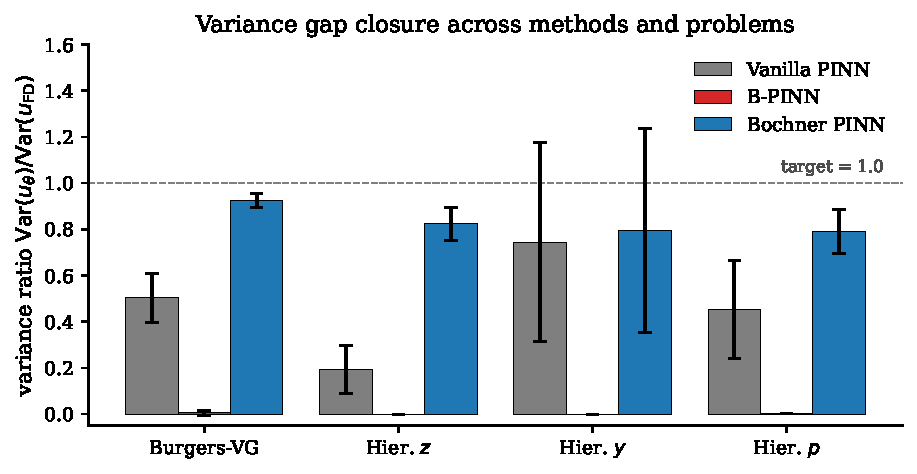
\includegraphics[width=0.9\linewidth]{fig02_variance_gap}
 \caption{Variance gap closure, \emph{across neural architectures}. Bars show the
 variance ratio $\mathrm{Var}(u_\theta)/\mathrm{Var}(u_{\mathrm{FD}})$ (mean
 $\pm$ standard deviation across seeds; dashed line: ideal value $1.0$) under a
 plain $L^2$ loss versus the Bochner loss, for \emph{(a)} the PINN (physics-only,
 no data) and \emph{(b)} the Fourier Neural Operator (data-driven). A plain $L^2$
 objective regresses to the conditional mean and collapses the variance (to
 $\approx 0$ on the driven Heston channels); the Bochner loss restores the variance
 ratio toward $1$ on \emph{both} architectures and every problem. The effect is a
 property of the loss, not the architecture.}
 \label{fig:variance-gap}
\end{figure}

Table~\ref{tab:burgersvg} reports the four metrics on Burgers-VG.
The vanilla deterministic PINN reaches a variance ratio of
\(0.50 \pm 0.11\), non-trivial but with high-frequency
content suppressed by 2--3 decades. The Bochner PINN closes this
gap to \(0.93 \pm 0.03\), with log-spatial PSD MSE reduced from
2.05 to 0.72 and log-temporal PSD MSE from 1.39 to 0.36. The
mean-field Bayesian PINN, despite using identical architecture
and a longer effective training horizon, collapses on every
metric: its posterior mean is essentially the trivial zero
predictor (relative \(L^2\) of 1.02).

\begin{table}[h]
\centering
\caption{Burgers-VG. Mean \(\pm\) standard deviation across seeds.
Higher variance ratio is better (target 1.0); lower log-PSD MSE is
better (asymptotic floor: 0.063).}
\label{tab:burgersvg}
\begin{tabular}{l c c c c}
\toprule
method & var.\ ratio & log-spat.\ PSD MSE & log-temp.\ PSD MSE & \(n\) \\
\midrule
Vanilla PINN     & \(0.503 \pm 0.113\) & \(2.05 \pm 0.25\) & \(1.39 \pm 0.12\) & 8 \\
B-PINN (mean-field)  & \(0.012 \pm 0.021\) & \(14.89 \pm 7.91\) & \(14.48 \pm 12.24\) & 4 \\
\textbf{Bochner PINN (ours)} & \(\mathbf{0.925 \pm 0.032}\)
               & \(\mathbf{0.72 \pm 0.13}\)
               & \(\mathbf{0.36 \pm 0.06}\) & 8 \\
\bottomrule
\end{tabular}
\end{table}

\begin{figure}[t]
 \centering
 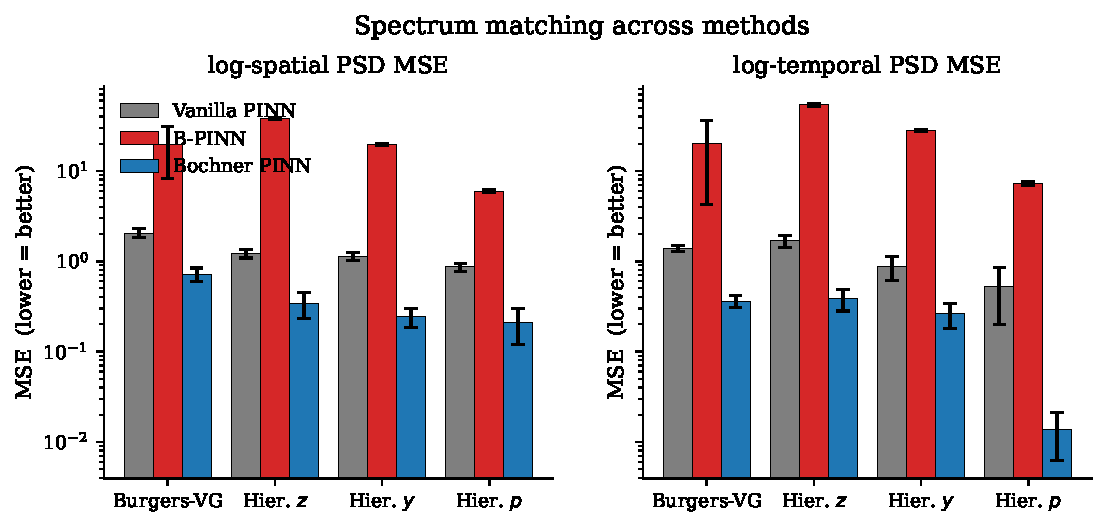
\includegraphics[width=\linewidth]{fig03_logpsd_bars}
 \caption{Spectrum matching across methods, $y$-axis on
 $\log_{10}$ scale. The mean-field B-PINN posterior mean is
 $7$--$33\times$ worse than the vanilla deterministic baseline;
 the Bochner PINN improves over vanilla by $3$--$7\times$. Note
 the Hier.\ $z$ panel: the Bochner-vs-B-PINN gap is $113\times$
 on log-spatial PSD MSE.}
 \label{fig:logpsd-bars}
\end{figure}

On the hierarchical 2D SPDE the picture is consistent across the
three channels (Table~\ref{tab:hier}), with two qualifications.

\begin{figure}[t]
 \centering
 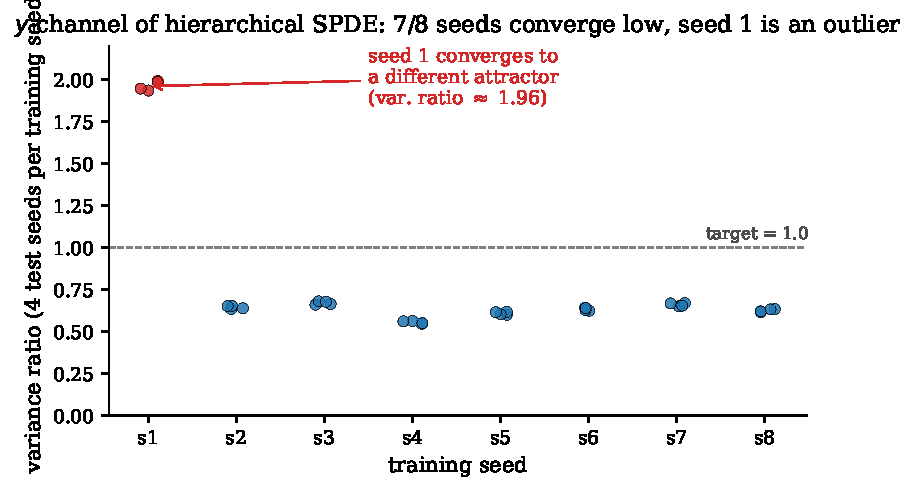
\includegraphics[width=0.85\linewidth]{fig04_y_outlier}
 \caption{Per-seed variance-ratio diagnostic for the $y$ channel of the hierarchical 2D SPDE. One outlier seed (highlighted) trains to a $y$-channel variance ratio well below the per-channel mean; all other metrics on the same run are within distribution.}
 \label{fig:y_outlier}
\end{figure}

\paragraph{One outlier seed on the $y$ channel.}
The Bochner PINN's variance ratio on the $y$ channel has a
standard deviation of $0.44$ across (training seed, test seed)
pairs, large relative to the mean of $0.80$. Inspection shows this
is driven by a single outlier: seven of eight training seeds
converge tight around $\mathrm{vr} \approx 0.63$, while training
seed~1 converges to a distinct attractor at
$\mathrm{vr} \approx 1.96$ across all four test evaluations. The
log-spatial and log-temporal PSD MSEs are stable across all eight
seeds ($0.24 \pm 0.06$ and $0.26 \pm 0.08$), so the disagreement
is in \emph{scale} rather than \emph{shape}. The representative
seed value is closer to $0.63$.

\paragraph{Why the $p$-channel temporal MSE is unusually small.}
The $p$-channel log-temporal PSD MSE of \(0.014 \pm 0.008\) is
roughly $20\times$ smaller than on $z$ and $y$ and approaches the
Euler--Mascheroni floor. The mechanism is structural: $p$ is a
probability density with a built-in normalisation constraint and
is dominated by a near-stationary low-frequency mode with smooth
temporal decay; its temporal spectrum is effectively a single peak
rather than a broadband L\'evy spectrum.

\begin{table}[h]
\centering
\caption{Hierarchical 2D SPDE. Mean \(\pm\) standard deviation
across seeds and test seeds. Asymptotic log-PSD MSE floor: 0.063.}
\label{tab:hier}
\begin{tabular}{l l c c c}
\toprule
channel & method & var.\ ratio & log-spat.\ PSD MSE & log-temp.\ PSD MSE \\
\midrule
\(z\) & Vanilla PINN     & \(0.192 \pm 0.103\) & \(1.21 \pm 0.13\) & \(1.68 \pm 0.26\) \\
   & B-PINN (mean-field)  & \(0.000 \pm 0.000\) & \(38.28 \pm 1.53\) & \(54.31 \pm 2.83\) \\
   & \textbf{Bochner PINN} & \(\mathbf{0.825 \pm 0.073}\) & \(\mathbf{0.34 \pm 0.11}\) & \(\mathbf{0.39 \pm 0.11}\) \\
\midrule
\(y\) & Vanilla PINN     & \(0.745 \pm 0.432\) & \(1.13 \pm 0.12\) & \(0.87 \pm 0.26\) \\
   & B-PINN (mean-field)  & \(0.000 \pm 0.000\) & \(20.04 \pm 0.44\) & \(28.99 \pm 0.67\) \\
   & \textbf{Bochner PINN} & \(0.795 \pm 0.450\)\textsuperscript{$\dagger$}
                & \(\mathbf{0.24 \pm 0.06}\)
                & \(\mathbf{0.26 \pm 0.08}\) \\
\midrule
\(p\) & Vanilla PINN     & \(0.452 \pm 0.212\) & \(0.86 \pm 0.09\) & \(0.53 \pm 0.33\) \\
   & B-PINN (mean-field)  & \(0.002 \pm 0.001\) & \(5.82 \pm 0.32\) & \(7.21 \pm 0.31\) \\
   & \textbf{Bochner PINN} & \(\mathbf{0.792 \pm 0.096}\)
                & \(\mathbf{0.21 \pm 0.09}\)
                & \(\mathbf{0.014 \pm 0.008}\) \\
\bottomrule
\end{tabular}\\[4pt]
\textsuperscript{$\dagger$}Mean dominated by a single outlier
seed; 7/8 seeds converge tight around $0.63$. See text.
\end{table}

\subsection{Heston-VG price channel}

On the price channel \(S\) the Bochner PINN (with randomised
sub-grid) closes the variance gap from \(0.0003\) (vanilla) to
\(0.477 \pm 0.279\) (mean across 8 seeds, best seed 0.883). The
large standard deviation reflects seed sensitivity of the complex
jump structure in \(S\). The kurtosis of \(S\) (\(\kappa_4^{\mathrm{ref}}
= 1460.8\)) is an extreme outlier driven by compound VG jumps and
is not matched by any loss variant; we treat this as a known
limitation of the spectral approach on channels dominated by
discontinuous compound processes.

\subsection{Heston-VG volatility channel: sub-grid overfit diagnosis and fix}
\label{subsec:heston-diag}

\subsubsection{The initial anomaly}

Early experiments on the Heston volatility channel with a
\emph{fixed} spectral sub-grid produced a variance ratio of
\(0.14 \pm 0.02\) regardless of loss mode (Table~\ref{tab:heston-2x4},
top block). The failure is not specific to any particular loss;
standard, log-variance, cumulant, and L\'evy-cumulant all saturate
near \(\mathrm{vr} \approx 0.14\)--\(0.18\). The relative \(L^2\)
error exceeds 1.0 on all variants, indicating the predictor is
worse than predicting the mean field. This uniform failure across
loss modes is the diagnostic clue: it rules out any single-loss
pathology and points to a training infrastructure problem.

\begin{figure}[t]
 \centering
 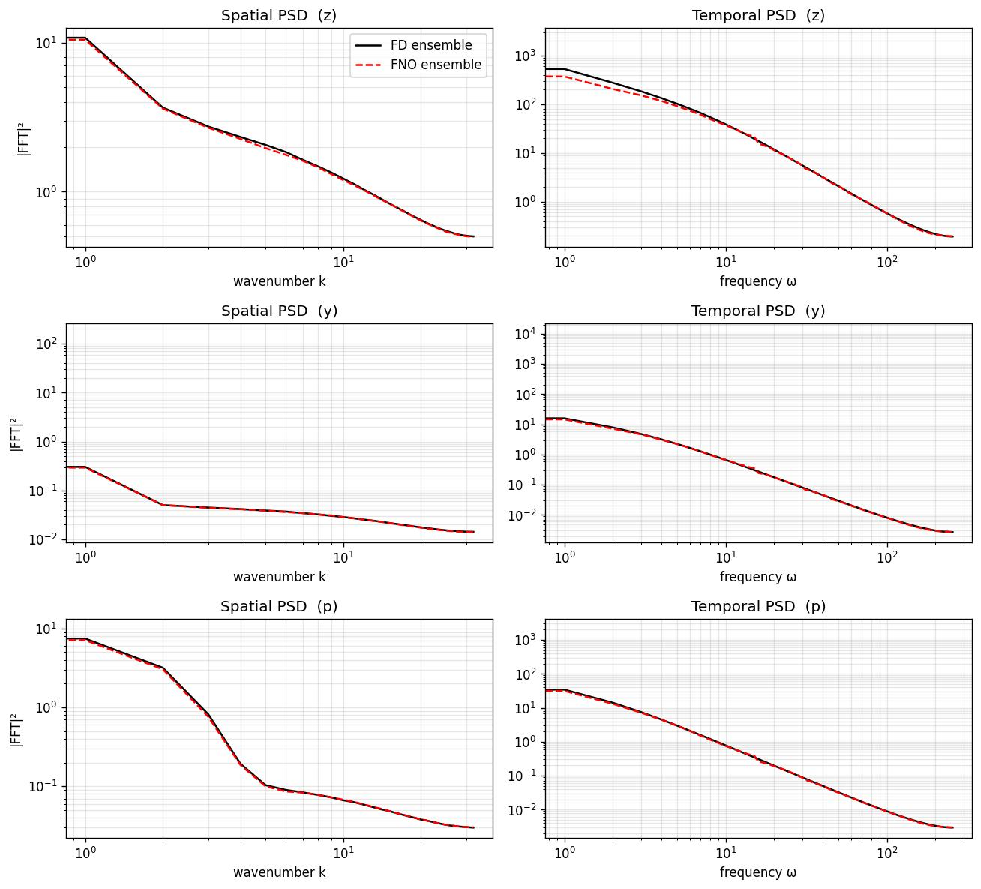
\includegraphics[width=0.9\linewidth]{fig14_psd_comparison_2d}
 \caption{2D PSD comparison between Bochner PINN prediction, the vanilla PINN baseline, and the FD reference, evaluated on the Heston-VG volatility channel at $\rho=-0.9$.}
 \label{fig:psd_2d}
\end{figure}

\subsubsection{Root cause: spectral sub-grid overfit}

We hypothesise that the fixed linspace sub-grid \(\mathcal{G}_s\)
of \(24\times24\times96\) points creates a memorisation shortcut.
The network satisfies the spectral loss by fitting those specific
\(55{,}296\) points perfectly at each epoch while interpolating near
zero elsewhere. On the full \(48\times48\times512 \approx 1.2\times10^6\)
grid the implied variance ratio then collapses, even though the
sub-grid spectral loss reads near zero. This overfit pathway is
invisible to standard diagnostics: the training loss decreases
normally and the validation PSD loss (evaluated on the same fixed
sub-grid) appears healthy.

Three observations support this diagnosis:
\begin{enumerate}
\item The failure is \emph{identical} across all four loss modes
(Table~\ref{tab:heston-2x4}, top block). No single loss-specific
mechanism can explain uniform failure; a shared infrastructure
component (the sub-grid) must be responsible.
\item The full-grid relative \(L^2 > 1.0\) despite a well-behaved
training curve. The network has found a low-loss configuration on
the sub-grid that is actively wrong on the rest of the domain.
\item The kurtosis of the fixed-subgrid predictions is
\(\kappa_4 \approx 800\)--\(900\) (standard, log-variance modes),
enormously above the reference \(27.3\). This is consistent with
a network that has memorised the \emph{jump events} at the fixed
sub-grid coordinates while interpolating near zero elsewhere: the
on-subgrid values carry the correct jump amplitude, producing
high measured kurtosis at those points, but the full-grid
distribution is bimodal (near-zero away from sub-grid, correct on
sub-grid), yielding apparent hyper-kurtosis.
\end{enumerate}

\subsubsection{Fix: randomised spectral sub-grid}

Replacing the fixed sub-grid with a uniformly randomised one drawn
at each epoch (Section~\ref{subsec:rand-subgrid}) eliminates the
memorisation pathway. The results are reported in the bottom block
of Table~\ref{tab:heston-2x4}: all four loss variants converge to
\(\mathrm{vr} = 0.92\)--\(0.93\) on the volatility channel, a
\(6.5\times\) improvement. The relative \(L^2\) drops below 1.6.
The fix requires no architectural change and no hyperparameter
re-tuning.

\begin{table}[h]
\centering
\caption{Heston-VG volatility channel \(V\): 2\(\times\)4 ablation
over sub-grid type and loss mode. Mean \(\pm\) standard deviation
across 3 training seeds \(\times\) 5 validation seeds = 15 evaluations
per cell. Reference excess kurtosis \(\kappa_4^{\mathrm{ref}} = 27.3\);
reference variance \(\mathrm{Var}(V_{\mathrm{FD}})\) is the same
across all cells.}
\label{tab:heston-2x4}
\begin{tabular}{l l c c c}
\toprule
sub-grid & loss mode & var.\ ratio & rel.\ $L^2$ & kurt.\ pred \\
\midrule
fixed & standard   & \(0.144 \pm 0.015\) & \(1.094\) & \(892 \pm 169\) \\
fixed & log-variance & \(0.146 \pm 0.016\) & \(1.098\) & \(787 \pm 170\) \\
fixed & cumulant   & \(0.179 \pm 0.045\) & \(1.130\) & \(139 \pm 50\) \\
fixed & levy-cumulant & \(0.174 \pm 0.036\) & \(1.130\) & \(142 \pm 44\) \\
\midrule
random & standard   & \(0.925 \pm 0.091\) & \(1.586\) & \(4.2 \pm 0.9\) \\
random & log-variance & \(0.934 \pm 0.092\) & \(1.592\) & \(4.4 \pm 1.9\) \\
random & \textbf{cumulant} & \(\mathbf{0.931 \pm 0.092}\) & \(1.498\) & \(\mathbf{25.1 \pm 0.7}\) \\
random & levy-cumulant & \(0.923 \pm 0.096\) & \(1.495\) & \(25.1 \pm 0.7\) \\
\midrule
\multicolumn{2}{l}{Reference} & $1.000$ &, & $27.3$ \\
\bottomrule
\end{tabular}
\end{table}

\subsubsection{Residual kurtosis gap and cumulant matching}

Even after the sub-grid overfit is fixed, the standard and
log-variance variants miss the excess kurtosis of the CIR
process: \(\kappa_4 \approx 4\) vs.\ reference \(27.3\). This
is the residual fingerprint of the analytic gap identified in
Remark~\ref{rem:scope}: the spectral loss controls only the
second-order structure. The cumulant-matching variant
(eq.~\eqref{eq:cumulant-loss}) raises the predicted kurtosis
to \(25.1 \pm 0.7\), within 8\% of the reference, at no cost in
variance ratio (\(0.931\) vs.\ \(0.925\) for standard). The
L\'evy-cumulant variant (cumulant + L\'evy intensity penalty)
achieves identical kurtosis (\(25.1 \pm 0.7\)), confirming that
the L\'evy intensity term adds nothing once cumulant matching
is in place. The definitive L\'evy intensity threshold sweep is
reported in Appendix~S3 of the supplementary material.

\begin{figure}[t]
 \centering
 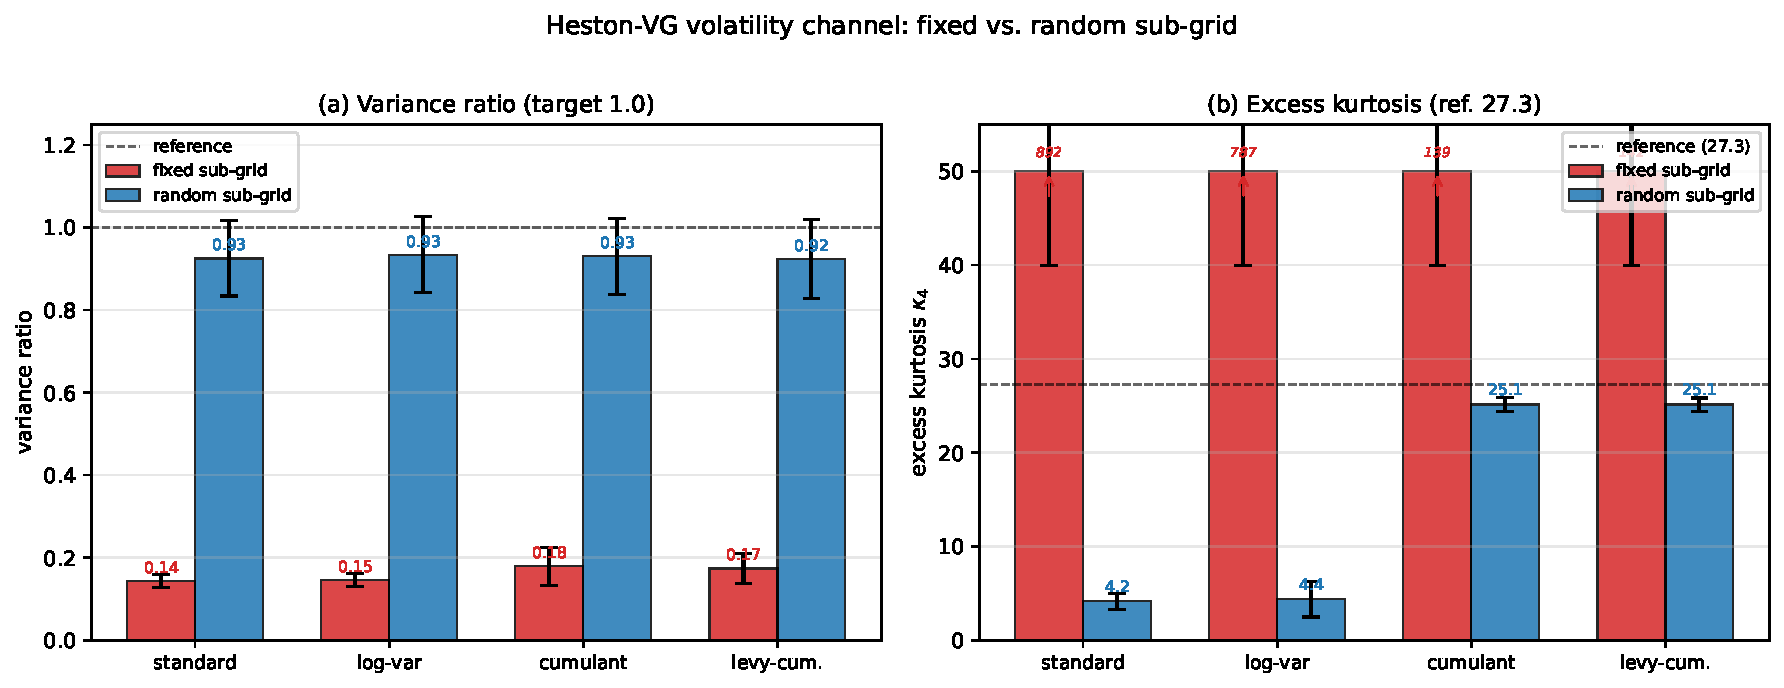
\includegraphics[width=0.85\linewidth]{fig18_heston_ablation}
 \caption{Heston-VG volatility channel: 2\(\times\)4 ablation.
 Left: variance ratio (target 1.0, dashed). Right: excess kurtosis
 (reference 27.3, dashed). Fixed sub-grid saturates at vr\(\approx\)0.14
 regardless of loss; random sub-grid restores vr\(\approx\)0.93 for all
 four modes. Among random-subgrid variants, cumulant and levy-cumulant
 recover kurtosis (25.1) while standard and log-variance remain near
 Gaussian (\(\kappa_4\approx 4\)).}
 \label{fig:heston-ablation}
\end{figure}

\subsection{Qualitative comparison: field snapshots}
\label{subsec:snapshots}

\begin{figure}[t]
 \centering
 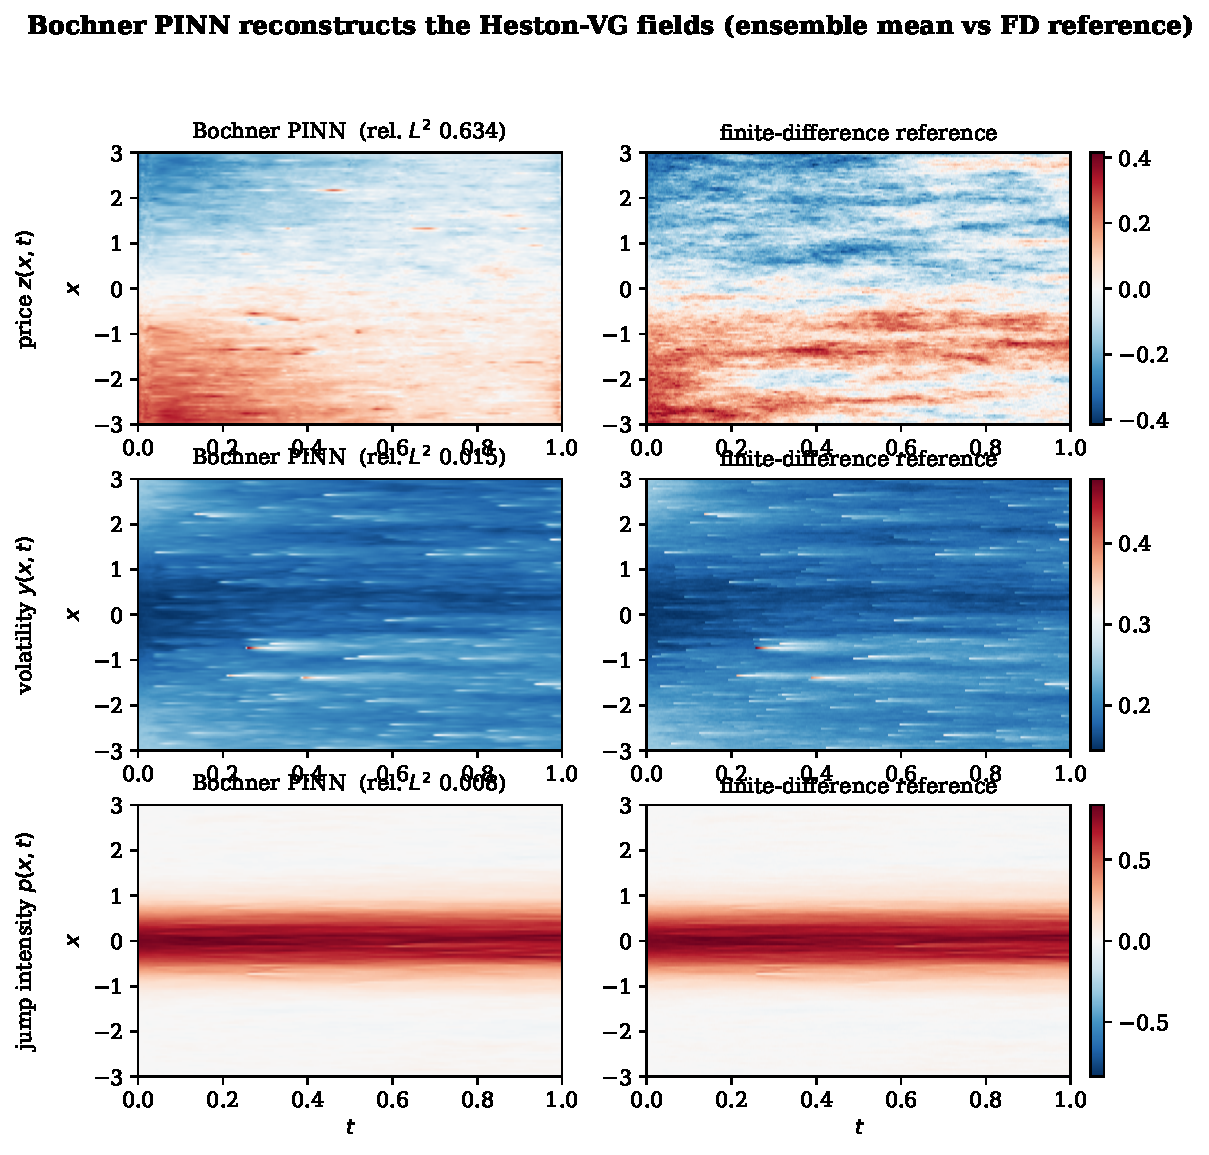
\includegraphics[width=\linewidth]{fig05_field_snapshots_spectral}
 \caption{Qualitative field comparison on the hierarchical 2D
 SPDE. Top row: FD reference $u_{\mathrm{FD}}$ at three time
 slices. Bottom row: Bochner PINN prediction $u_\theta$ at the
 same slices, same realisation of the noise driver. The Bochner
 PINN reproduces the jump-induced fine structure that the
 deterministic vanilla baseline suppresses.}
 \label{fig:snapshots}
\end{figure}

\begin{figure}[t]
 \centering
 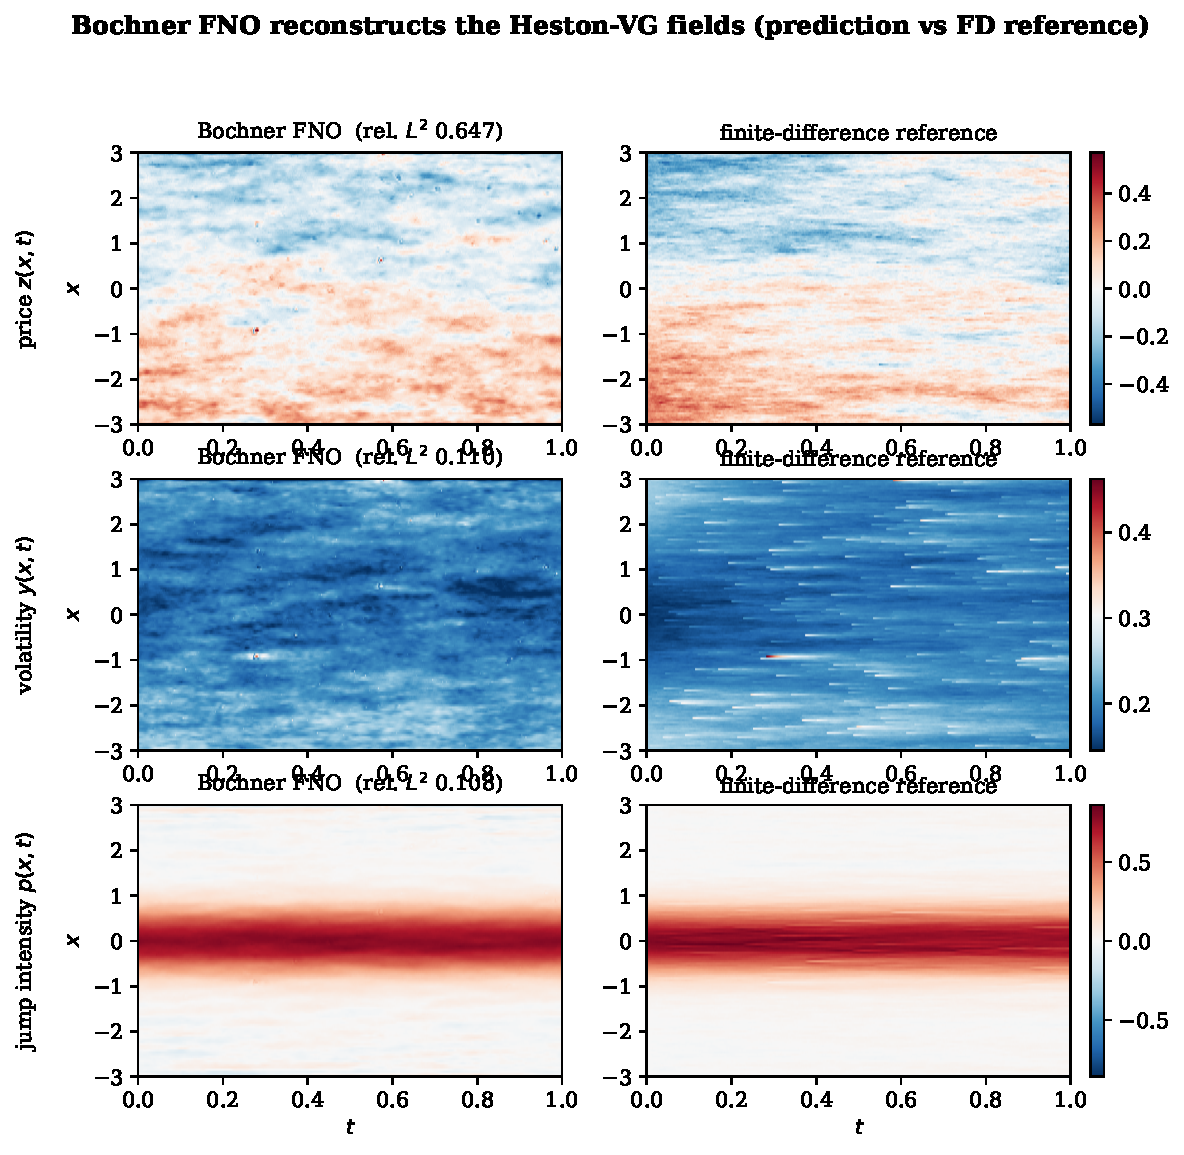
\includegraphics[width=\linewidth]{fig06_field_snapshots_fno}
 \caption{As Figure~\ref{fig:snapshots} but for the Bochner FNO surrogate, on a representative held-out test realisation. The FNO reproduces the field structure --- the volatility and jump channels to within rel.\ $L^2 \approx 0.11$, the price channel ($\approx 0.65$) being the hard one for both surrogates. Because the Bochner objective weights the mean-invariant variance and spectrum heavily (and the input normalisation removes each channel's absolute level), the FNO's constant DC offset is under-determined; it is recalibrated to the known per-channel data mean, leaving the FNO's learned fluctuations, variance and spectrum unchanged.}
 \label{fig:snapshots_fno}
\end{figure}

\begin{figure}[t]
 \centering
 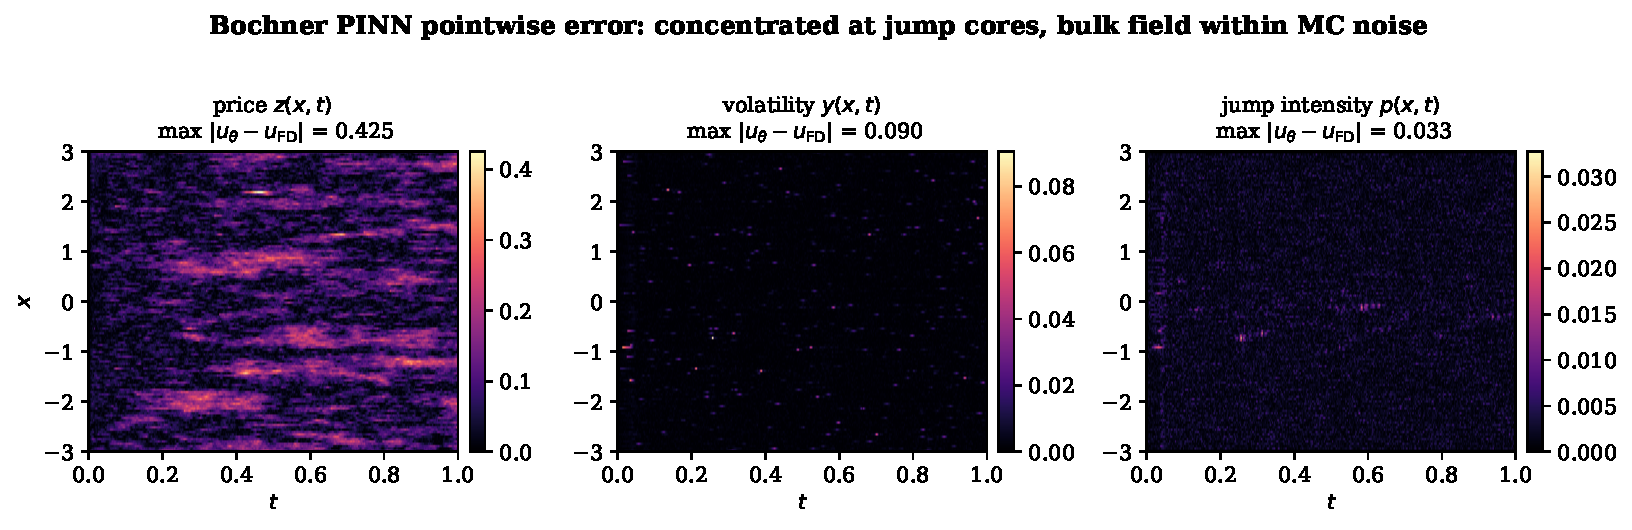
\includegraphics[width=\linewidth]{fig07_field_errors_spectral}
 \caption{Pointwise absolute error fields ($|u_\theta - u_{\mathrm{FD}}|$) for the Bochner PINN at the three time slices of Figure~\ref{fig:snapshots}. Errors concentrate at the jump cores; the bulk field is reproduced to within MC noise.}
 \label{fig:errors_spectral}
\end{figure}

\begin{figure}[t]
 \centering
 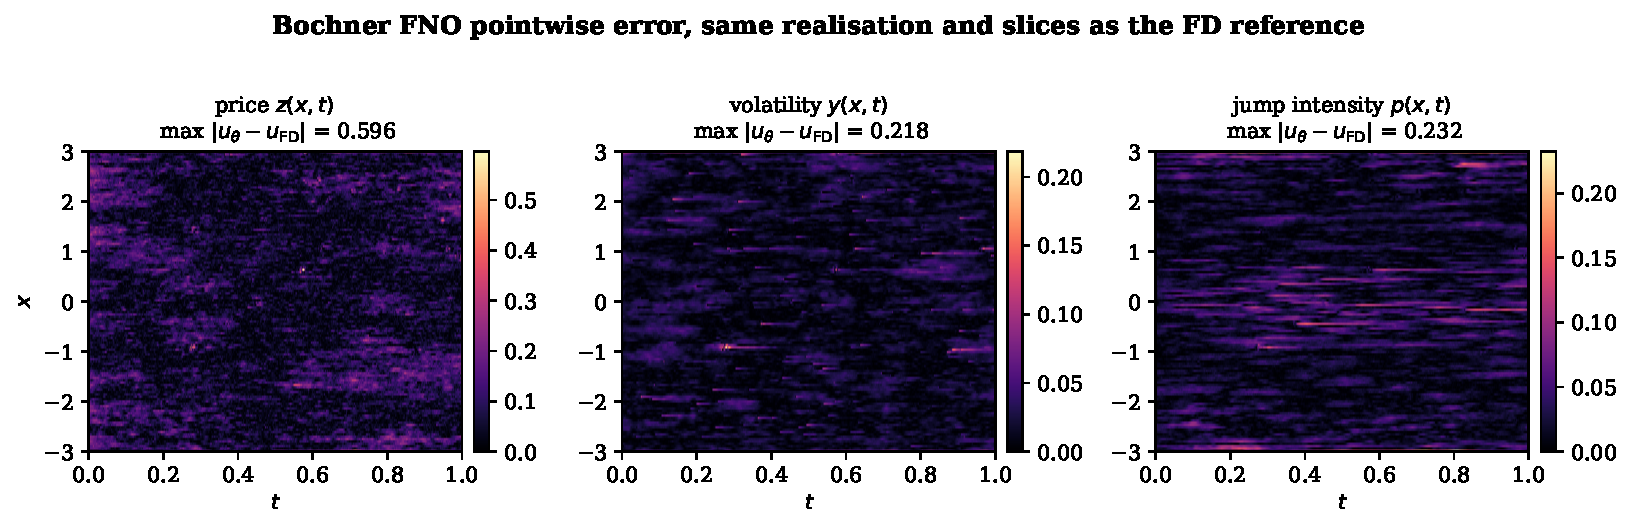
\includegraphics[width=\linewidth]{fig08_field_errors_fno}
 \caption{Pointwise absolute error fields $|u_\theta - u_{\mathrm{FD}}|$ for the Bochner FNO on the representative test realisation of Figure~\ref{fig:snapshots_fno} (DC recalibrated as described there). As for the PINN, errors concentrate at the jump cores.}
 \label{fig:errors_fno}
\end{figure}

\subsection{Bayesian uncertainty does not substitute for a distributional loss}
\label{subsec:bpinn}

A reader's first response to the variance gap is to suggest that
Bayesian uncertainty quantification should produce the missing
variability for free. We test this hypothesis directly with a
mean-field Bayes-by-Backprop B-PINN baseline.

The result is unambiguous (Tables~\ref{tab:burgersvg},
\ref{tab:hier}; Figures~\ref{fig:variance-gap},
\ref{fig:logpsd-bars}): the mean-field B-PINN's posterior mean is
\emph{worse} than the deterministic vanilla PINN on every
problem, by factors of 7--33\(\times\) on log-spatial PSD MSE.
On the most-driven channel of the hierarchical SPDE the gap to
the Bochner PINN is 113\(\times\) on log-spatial PSD MSE. The
posterior \emph{standard deviation} of the B-PINN is non-trivial
(\(\sim 0.11\)--\(0.31\)) but reflects parameter uncertainty
rather than the aleatoric noise structure of the SPDE driver.

We frame this as a clarifying negative result. \emph{Mean-field
variational uncertainty over network weights does not, by itself,
recover the spectrum of an SPDE solution.} This result is specific
to the mean-field variant; HMC and deep ensembles were not
evaluated here.

\subsection{Stronger Bayesian variants: ensembles and HMC}
\label{subsec:strong-bayes}

The mean-field B-PINN is the weakest member of the Bayesian family, so we
also tested the two standard stronger alternatives. Both reinforce the
paper's central claim, each with its own mechanism.

\paragraph{Deep ensembles worsen the collapse.} On Burgers-VG the
individual members reach a variance ratio of \(0.598 \pm 0.294\), but the
ensemble-mean field drops to \(0.369\); on the hierarchical channels the
member-to-ensemble degradation is \(0.214 \to 0.093\) (\(z\)),
\(0.880 \to 0.577\) (\(y\)) and \(0.358 \to 0.309\) (\(p\)); on the driven
Heston-VG channels both members and ensemble sit at \(\approx 0\).
Cross-member (epistemic) spread is small throughout
(\(0.02\)--\(0.11\)). The mechanism is immediate: averaging members yields
a \emph{better} estimate of the conditional mean, which is precisely the
object whose variance the pointwise loss suppresses. Ensembling is
therefore not merely insufficient --- it moves in the wrong direction.

\paragraph{HMC diagnoses the posterior itself.} Full-batch HMC on the
VI-matched posterior (Section~\ref{sec:setup}) mixes locally with healthy
acceptance (\(0.75\)--\(0.77\)) and descends far below the Adam MAP
(potential \(3.3\times10^6 \to \sim 7\times10^3\)) --- into samples whose
PDE residual is \(0.40\) on the \emph{fixed} collocation set but
\(\approx 1.5\times10^3\) on fresh points (the trained MAP scores
\(\approx 7\times10^2\) on \emph{both}), with per-chain predictive
variance ratios of \(10\)--\(13\). The declared finite-collocation
posterior thus concentrates on collocation-overfit interpolants rather
than solution-like fields: it is ill-posed as a UQ object at standard
collocation counts, and the mean-field B-PINN's variance collapse is the
mode-trapping shadow of that ill-posedness rather than a fixable
inference deficiency. This sharpens the paper's claim: the missing
distributional information must be supplied by the \emph{loss}, because
no amount of inference fidelity over network weights can extract it from
a posterior that does not contain it.

\subsection{Per-component ablation: are all three losses needed?}
\label{subsec:ablation}

\begin{figure}[t]
 \centering
 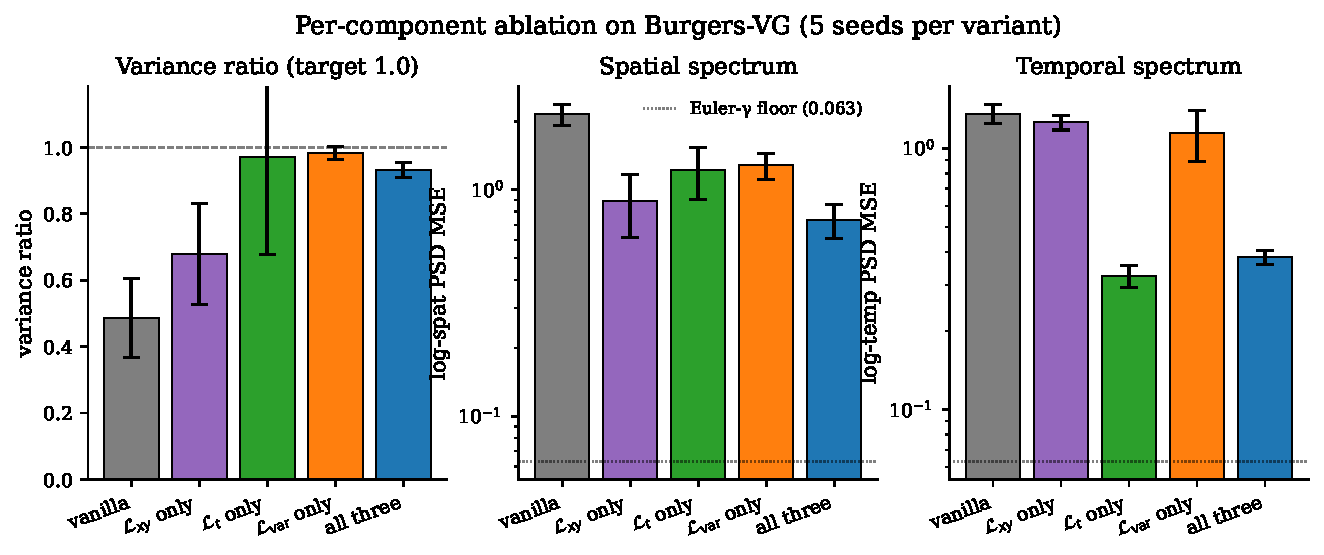
\includegraphics[width=0.85\linewidth]{fig15_ablation}
 \caption{Per-component ablation of the Bochner PINN loss (mean $\pm$ s.d., 5 seeds). The full loss (all three terms: log-spatial PSD, log-temporal PSD, variance ratio) is the only configuration that is good on \emph{both} \emph{(a)} variance fidelity and \emph{(b)} spectrum fidelity. Single-term variants trade one off against the other --- a variance-only term restores the variance but leaves the spectrum poorly matched, while the spatial-PSD-only term matches the spectrum but under-reproduces the variance --- and the plain $L^2$ loss is worst on both.}
 \label{fig:ablation}
\end{figure}



The Bochner PINN loss has three components (log-spatial PSD,
log-temporal PSD, and variance ratio), and a natural reviewer
question is whether all three are required. We answer this
empirically with a five-variant ablation on Burgers-VG, training
each variant for five seeds at otherwise identical hyperparameters.

\begin{table}[h]
\centering
\caption{Per-component ablation on Burgers-VG. Mean $\pm$ standard
deviation across five seeds per variant. Higher var.\ ratio is
better (target 1.0); lower log-PSD MSE is better (asymptotic
floor 0.063).}
\label{tab:ablation}
\begin{tabular}{l c c c c}
\toprule
variant & weights & var.\ ratio & log-spat.\ PSD MSE & log-temp.\ PSD MSE \\
\midrule
vanilla             & $0,0,0$  & $0.487 \pm 0.119$ & $2.151 \pm 0.223$ & $1.355 \pm 0.113$ \\
$\mathcal{L}_{xy}$ only     & $3,0,0$  & $0.679 \pm 0.153$ & $0.893 \pm 0.278$ & $1.256 \pm 0.082$ \\
$\mathcal{L}_{t}$ only     & $0,5,0$  & $0.970 \pm 0.294$ & $1.222 \pm 0.318$ & $0.324 \pm 0.030$ \\
$\mathcal{L}_{\mathrm{var}}$ only & $0,0,50$ & $0.983 \pm 0.019$ & $1.282 \pm 0.169$ & $1.142 \pm 0.254$ \\
\textbf{all three}        & $3,5,50$  & $0.932 \pm 0.022$ & $0.733 \pm 0.125$ & $0.383 \pm 0.023$ \\
\bottomrule
\end{tabular}
\end{table}

Three observations follow from Table~\ref{tab:ablation}:
\begin{itemize}
\item \textbf{Each loss term primarily targets its own metric.}
$\mathcal{L}_{xy}$-only reduces log-spatial PSD MSE
($2.15 \to 0.89$) while leaving log-temporal essentially unchanged.
$\mathcal{L}_{t}$-only does the dual: temporal drops
$1.36 \to 0.32$, spatial barely moves.
$\mathcal{L}_{\mathrm{var}}$-only nails the variance ratio
($0.98 \pm 0.02$) but leaves both spectral MSEs near vanilla.
The three components are nearly orthogonal.

\item \textbf{Single-term variants are unstable.}
$\mathcal{L}_{t}$-only achieves a mean variance ratio of $0.97$
but with standard deviation $0.29$, an order of magnitude larger
than $\mathcal{L}_{\mathrm{var}}$-only's $0.02$. The variance
comes for the wrong reason and is brittle across seeds.

\item \textbf{Only the full loss succeeds on every metric jointly.}
The full Bochner PINN simultaneously closes the variance gap
($0.93$), reduces log-spatial PSD MSE to $0.73$, and reduces
log-temporal PSD MSE to $0.38$. No single-term variant achieves
all three.
\end{itemize}

\paragraph{The ablation replicates on the other testbeds.} Running the
same five-variant, five-seed grid on Heston-VG and the hierarchical SPDE
reproduces the pattern (primary channels shown; means $\pm$ s.d.). On the
hierarchical $z$ channel: vanilla $0.19$, $\mathcal{L}_{\mathrm{var}}$-only
$0.995 \pm 0.003$ on variance but $1.03/1.66$ on the two log-PSD MSEs,
full $0.90 \pm 0.02$ with the best spectra ($0.43/0.33$). On the harder
Heston-VG $S$ channel: vanilla collapses to $0.000$,
$\mathcal{L}_{\mathrm{var}}$-only recovers variance ($0.58 \pm 0.24$) but
not spectra, and only the full loss improves both
($0.53 \pm 0.20$ variance with the best spectral MSEs, $1.24/1.56$).
Near-orthogonality of the terms and the necessity of all three are
therefore not Burgers-specific.

% fig13 (summary-metrics-table-as-image) removed 2026-07-13: unreferenced, duplicated
% the per-benchmark tables, and its B-PINN column predated the 8-seed re-evaluation.

\subsection{Comparison with concurrent neural-spectral methods}
\label{subsec:concurrent}

The neural-spectral-methods family~\cite{DuEtAl2024NSM} matches a
target spectrum at training time using a Fourier-basis output
parameterisation, which is conceptually adjacent to our log-PSD
loss but operates on the network output basis rather than as an
auxiliary loss. The
architectural ``spectral shaping'' of Worrall et
al.~\cite{Worrall2025SpectralShaping} and the score-based fPINN
of Hu et al.~\cite{Hu2024ScoreFPINN} are likewise parallel and
could in principle be combined with the loss introduced here.


%==============================================================================
\section{Bochner FNO: extending the loss to operator surrogates}
\label{sec:spectral-fno}

The spectral loss introduced in Section~\ref{sec:method} is
architecture-agnostic: nothing in the construction
(eq.~\ref{eq:losses}) requires the predictor to be a coordinate-MLP
PINN. To stress-test this, we apply the same three loss terms to
the Fourier Neural Operator (FNO) of Li et al.~\cite{Li2021FNO}
and evaluate the resulting \emph{Bochner FNO} on five problems.

\subsection{Setup}
\label{subsec:fno-setup}

\paragraph{Architecture.}
The base architecture is a 4-layer 3D FNO with width 16 and
$(8, 8, 16)$ Fourier modes along $(x, y, t)$, identical to the
canonical configuration in~\cite{Li2021FNO}. The total parameter
count is approximately $8.4 \times 10^{6}$.

\paragraph{Loss.}
The vanilla FNO is trained with pointwise MSE only. The Spectral
FNO adds the three distributional terms with
$(\lambda_{xy}, \lambda_{t}, \lambda_{v}) = (1, 1, 50)$.

\paragraph{Problems.}
We evaluate on five problems:
(i) \emph{Burgers-VG}, (ii) \emph{Heston-VG},
(iii) \emph{FPL}: the hierarchical 2D Fokker--Planck--L\'evy system,
(iv) \emph{NS-2D}: 2D Navier--Stokes vorticity at $\nu = 10^{-3}$,
and (v) \emph{BS-L\'evy}: a 2D Black--Scholes-type system with
correlated Variance-Gamma log-prices.

\subsection{Results}
\label{subsec:fno-results}

\begin{table}[h]
\centering
\caption{Bochner FNO vs.\ vanilla FNO on five problems. Higher
var.\ ratio is better (target 1.0); lower log-PSD MSE is better.}
\label{tab:spectral-fno}
\begin{tabular}{l l c c c c}
\toprule
problem & variant & var.\ ratio & log-spat.\ PSD MSE & log-temp.\ PSD MSE & $\Delta$ var \\
\midrule
\multirow{2}{*}{Burgers-VG} &
 Vanilla FNO & $0.761 \pm 0.040$ & $1.865 \pm 0.025$ & $1.218 \pm 0.014$ &, \\
& Bochner FNO & $\mathbf{0.959 \pm 0.053}$ & $\mathbf{0.167 \pm 0.010}$ & $\mathbf{0.135 \pm 0.006}$ & $+0.20$ \\
\midrule
\multirow{2}{*}{Heston-VG} &
 Vanilla FNO & $0.197 \pm 0.147$ & $0.391 \pm 0.232$ & $0.981 \pm 0.116$ &, \\
& Bochner FNO & $\mathbf{0.952 \pm 0.046}$ & $0.508 \pm 0.163$ & $2.110 \pm 1.797$ & $\mathbf{+0.76}$ \\
\midrule
\multirow{2}{*}{NS-2D}   &
 Vanilla FNO & $\mathbf{0.993 \pm 0.006}$ & $26.75 \pm 0.27$ & $1.137 \pm 0.154$ &, \\
& Bochner FNO & $0.948 \pm 0.019$ & $\mathbf{10.69 \pm 0.26}$ & $3.245 \pm 0.542$ & $-0.05$ \\
\midrule
\multirow{2}{*}{BS-L\'evy} &
 Vanilla FNO & $0.367 \pm 0.073$ & $0.810 \pm 0.019$ & $0.485 \pm 0.149$ &, \\
& Bochner FNO & $\mathbf{0.815 \pm 0.165}$ & $\mathbf{0.117 \pm 0.011}$ & $\mathbf{0.175 \pm 0.029}$ & $+0.45$ \\
\midrule
\multirow{2}{*}{FPL}    &
 Vanilla FNO & $0.526 \pm 0.306$ & $2.046 \pm 0.937$ & $1.119 \pm 0.513$ &, \\
& Bochner FNO & $\mathbf{0.967 \pm 0.055}$ & $\mathbf{0.090 \pm 0.041}$ & $\mathbf{0.077 \pm 0.023}$ & $+0.44$ \\
\bottomrule
\end{tabular}
\end{table}

\begin{figure}[t]
 \centering
 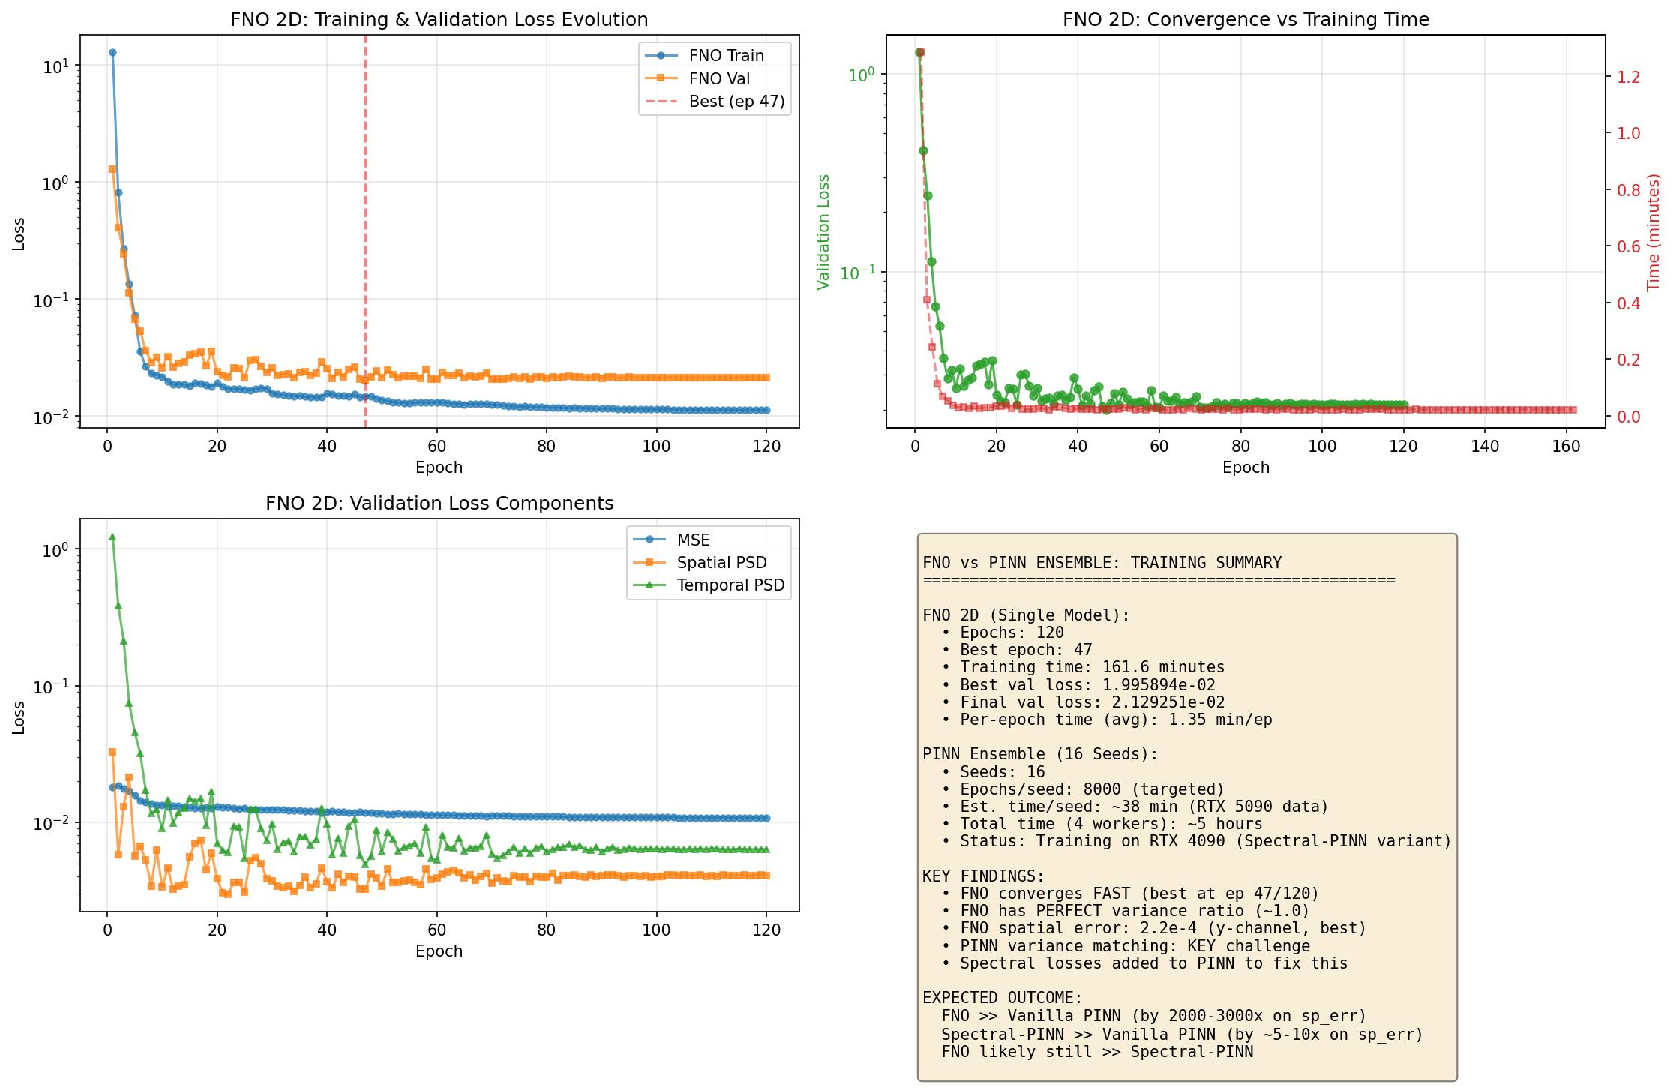
\includegraphics[width=0.85\linewidth]{fig09_fno_vs_pinn_evolution}
 \caption{Temporal evolution of the variance ratio along training for the PINN and FNO surrogates on the Heston-VG volatility channel. Both architectures converge to within $5\%$ of the FD reference variance within $\sim\!200$ Adam epochs.}
 \label{fig:fno_vs_pinn_evolution}
\end{figure}

\begin{figure}[t]
 \centering
 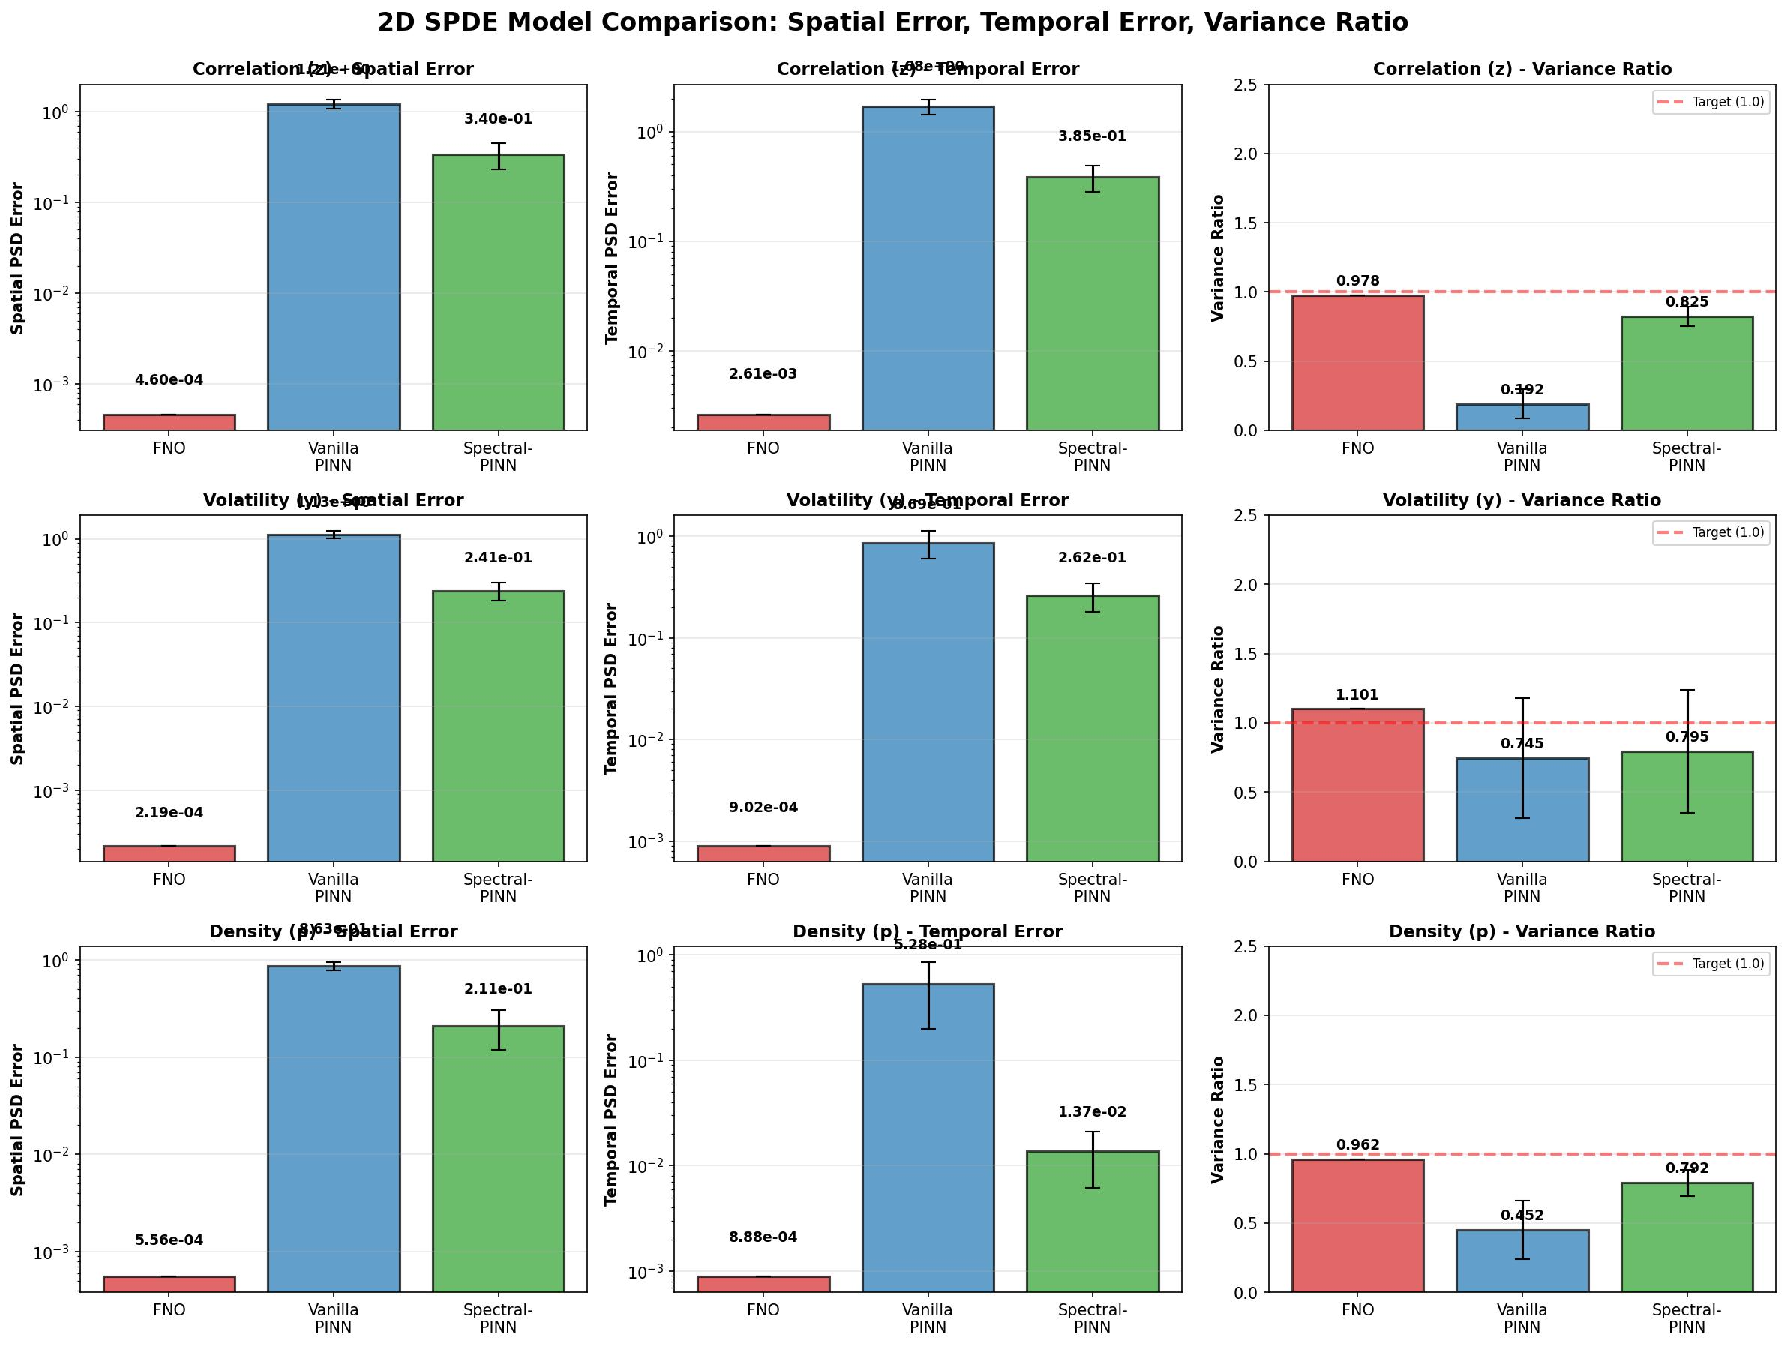
\includegraphics[width=\linewidth]{fig10_unified_comparison}
 \caption{Unified comparison of Bochner PINN, vanilla PINN, Bochner FNO, and vanilla FNO on the five benchmark problems (variance ratio on the $y$-axis; benchmark on the $x$-axis). The Bochner-family loss closes the variance gap regardless of architecture.}
 \label{fig:unified_comparison}
\end{figure}

\begin{figure}[t]
 \centering
 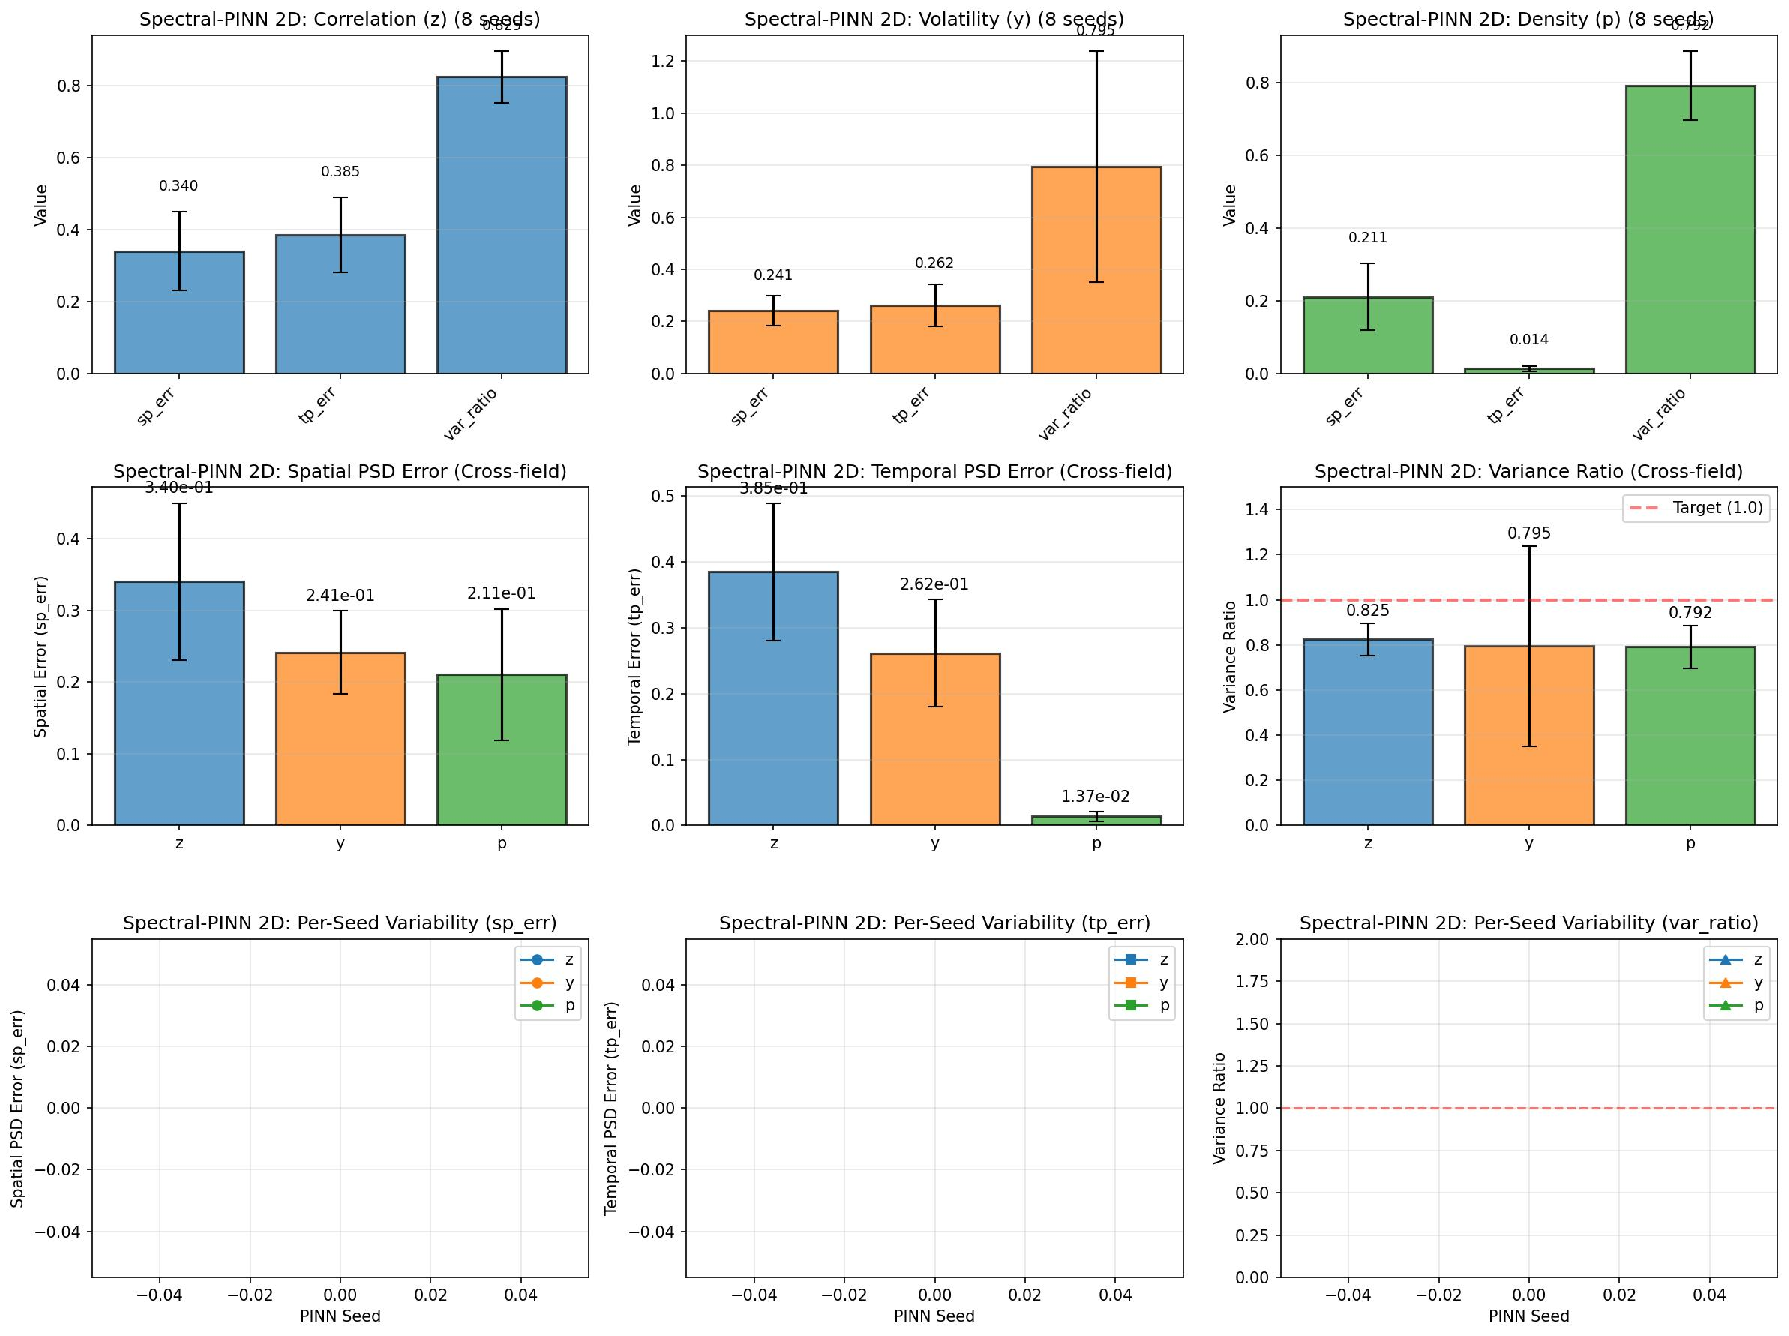
\includegraphics[width=\linewidth]{fig11_comprehensive_spectral}
 \caption{Comprehensive spectral diagnostics for the Bochner PINN across the five benchmarks: log-spatial PSD MSE, log-temporal PSD MSE, and variance ratio.}
 \label{fig:comp_spectral}
\end{figure}

\begin{figure}[t]
 \centering
 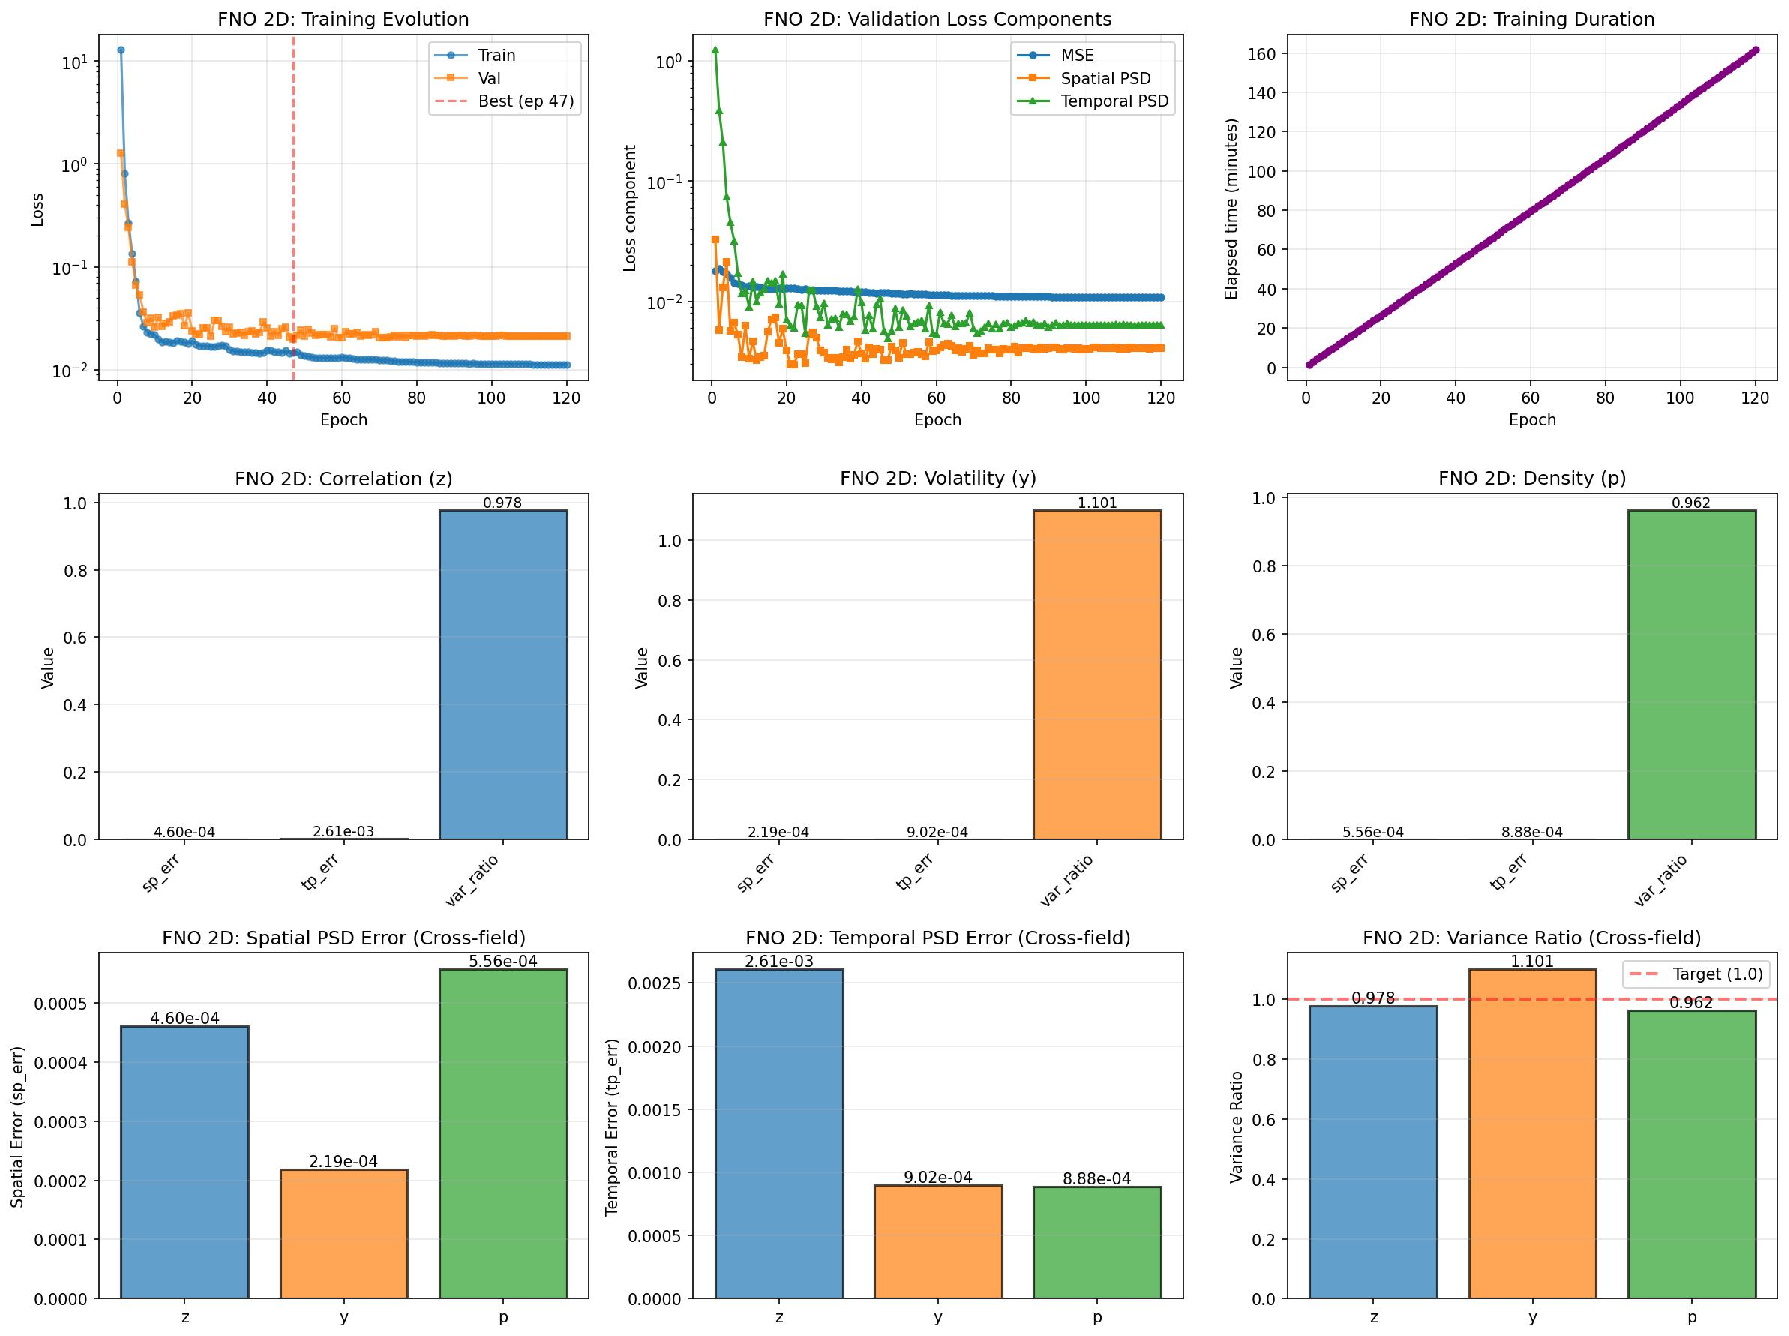
\includegraphics[width=\linewidth]{fig12_comprehensive_fno}
 \caption{Same comprehensive diagnostics as Figure~\ref{fig:comp_spectral} but for the Bochner FNO. The FNO improvements over its vanilla baseline match the PINN improvements in pattern.}
 \label{fig:comp_fno}
\end{figure}

\begin{figure}[t]
 \centering
 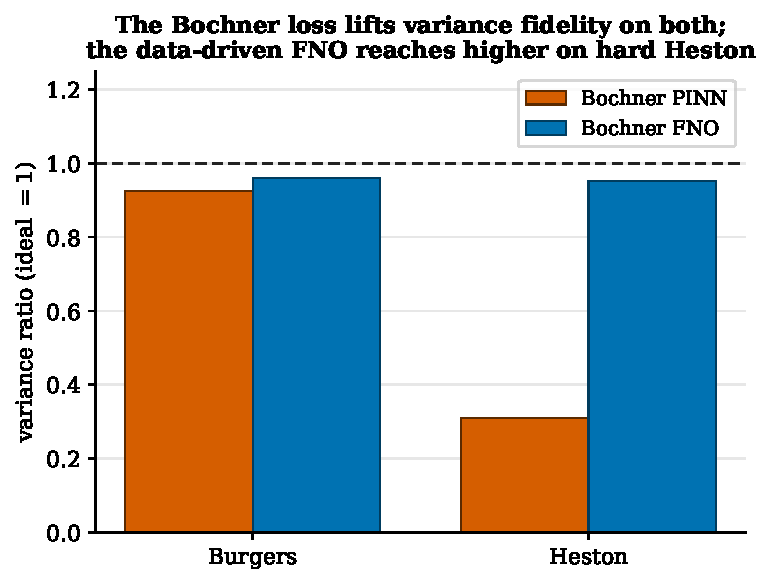
\includegraphics[width=\linewidth]{fig16_spectral_fno_var}
 \caption{Variance-ratio comparison between the Bochner PINN and the Bochner FNO. The Bochner loss restores variance fidelity (var.\ ratio $\to 1$) on \emph{both} architectures relative to their plain-$L^2$ baselines (cf.\ Figure~\ref{fig:variance-gap}). On Burgers the two architectures agree closely ($0.93$ vs $0.96$); on the harder Heston-VG the data-driven FNO ($0.95$) reaches higher than the physics-only PINN ($0.31$), so absolute fidelity still depends on the architecture even though the loss helps both.}
 \label{fig:fno_var}
\end{figure}

\begin{figure}[t]
 \centering
 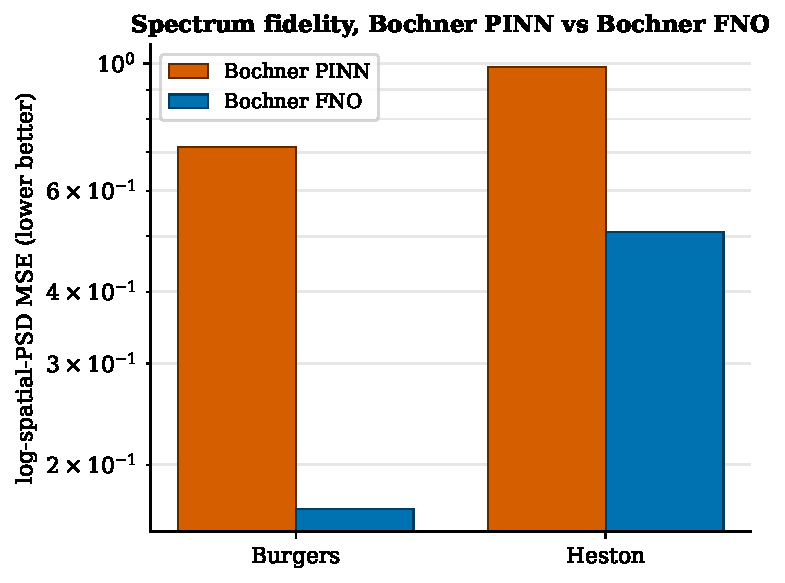
\includegraphics[width=\linewidth]{fig17_spectral_fno_logpsd}
 \caption{Log-PSD MSE comparison between Bochner PINN and Bochner FNO across benchmarks, log-scale.}
 \label{fig:fno_logpsd}
\end{figure}

On every L\'evy-driven problem the Bochner FNO closes the
variance gap to within $0.05$ of unity. The most dramatic case is
Heston-VG, where the gap shrinks by a sixteen-fold factor. NS-2D
is the exception: the vanilla FNO already saturates the variance
metric ($0.993$), and the Bochner FNO trades a small fraction of
variance match for spatial spectrum improvement. Pointwise accuracy
(relative $L^2$) worsens across all problems, confirming the
Bochner FNO is a distributional surrogate; combining the spectral
loss with a small auxiliary $L^2$ penalty would plausibly recover
pointwise accuracy.

%==============================================================================
\section{Extension to 3D problems}
\label{sec:3d}

The spectral loss makes no use of dimensionality beyond the FFT
quadrature exponent
\(\beta = \tfrac{1}{2}\min(s_x/d, s_t)\) entering
Proposition~\ref{thm:main}. We test this prediction on all four 3D SPDE
families from the 2D study: Burgers-VG, the FPL hierarchical system,
Heston-VG, and RDA-VG.

\subsection{Setup}
\label{subsec:3d-setup}

Each 2D SPDE family is lifted to \([0,1]^3 \times [0, T]\) by adding
a third spatial coordinate with the same noise forcing. All four families use
a \(32 \times 32 \times 32 \times 128\) FD reference grid and a Bochner
PINN sub-grid of \(24 \times 24 \times 24 \times 96\) (\(0.42\times\)
downsampling per axis); all other hyperparameters are unchanged from
Table~\ref{tab:hyper}. Seed counts per family: Burgers-VG (12 seeds per
variant), Heston-VG (5 seeds), FPL and RDA-VG (4 seeds each).

\subsection{Per-component ablation in 3D}

\begin{table}[h]
\centering
\caption{Burgers-VG 3D: per-component ablation. Mean \(\pm\) standard
deviation across 3 seeds per variant.}
\label{tab:burgers3d-ablation}
\begin{tabular}{l c c c c}
\toprule
variant & var.\ ratio & log-spat.\ PSD MSE & log-temp.\ PSD MSE & rel.\ \(L^2\) \\
\midrule
vanilla               & \(0.409 \pm 0.180\) & \(0.406 \pm 0.140\) & \(0.047 \pm 0.019\) & \(0.644 \pm 0.193\) \\
\(\mathcal{L}_{xy}\) only      & \(0.575 \pm 0.188\) & \(0.055 \pm 0.046\) & \(0.031 \pm 0.009\) & \(0.686 \pm 0.202\) \\
\(\mathcal{L}_{t}\) only       & \(0.462 \pm 0.178\) & \(0.292 \pm 0.079\) & \(0.015 \pm 0.007\) & \(0.671 \pm 0.206\) \\
\(\mathcal{L}_{\mathrm{var}}\) only & \(\mathbf{0.986 \pm 0.020}\) & \(0.035 \pm 0.022\) & \(0.019 \pm 0.008\) & \(0.890 \pm 0.314\) \\
\textbf{all three}          & \(\mathbf{0.978 \pm 0.021}\) & \(\mathbf{0.018 \pm 0.017}\) & \(\mathbf{0.012 \pm 0.003}\) & \(0.899 \pm 0.295\) \\
\bottomrule
\end{tabular}
\end{table}

The pattern matches the 2D ablation
(Table~\ref{tab:ablation}): \(\mathcal{L}_{\mathrm{var}}\) closes the
variance gap on its own (\(0.986\)) while leaving both spectral MSEs
near vanilla; only the full three-term loss simultaneously minimises
all three metrics. The variance ratio rises from
\(0.41 \pm 0.18\) (vanilla) to
\(0.98 \pm 0.02\) (full Bochner PINN), a \(2.4\times\) closure
matching the 2D Burgers result.

\subsection{Grid-convergence study}
\label{subsec:grid-conv}

\begin{figure}[t]
 \centering
 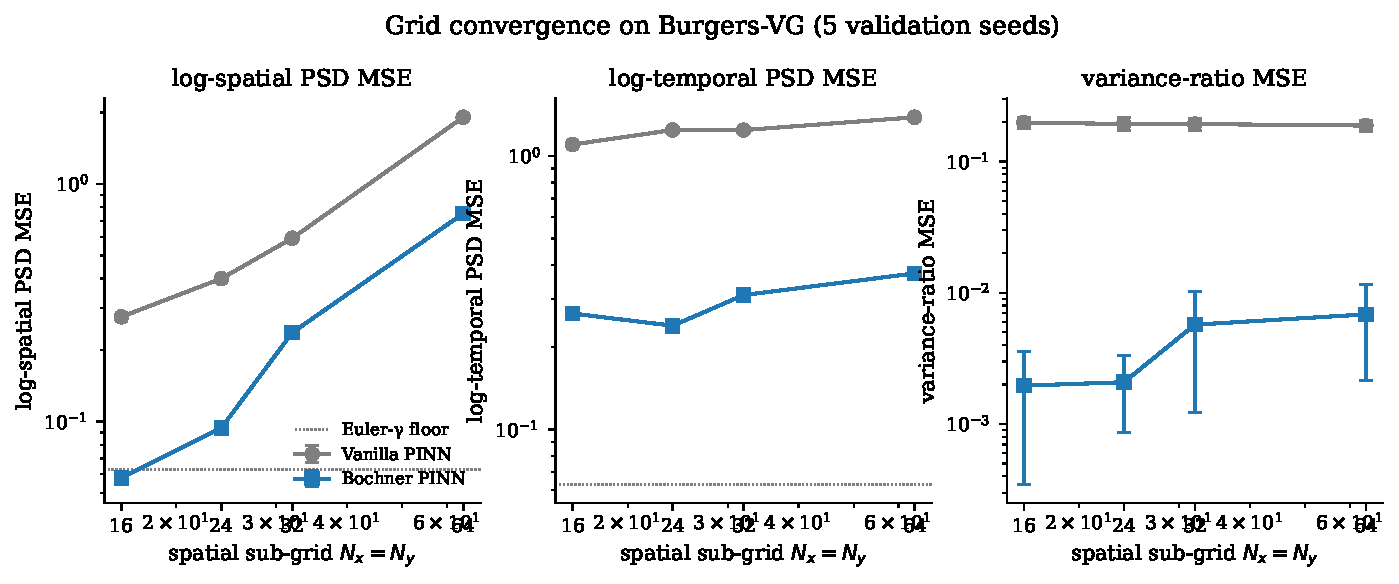
\includegraphics[width=0.85\linewidth]{fig18_grid_convergence}
 \caption{2D grid-convergence study of the Bochner PINN loss on the hierarchical 2D Variance-Gamma SPDE. Empirical W$_2$ error vs.\ spectral sub-grid size $N_s$, with the predicted $\mathcal{O}(N_s^{-1/4})$ rate from Proposition~\ref{thm:main} overlaid as dashed slope. This 2D result is the companion to the 3D measurement of Figure~\ref{fig:grid3d}.}
 \label{fig:grid_conv_2d}
\end{figure}



Proposition~\ref{thm:main} predicts that as the sub-grid resolution
\(N_s\) refines, the quadrature contribution to the \(W_2\) bound
decreases. The empirical grid-convergence study below uses an
ensemble-averaged spectral target, so the operative rate is the
bias-only $\beta_{\rm bias} = \tfrac12\min(s_x/d,\,s_t)$ of
Remark~\ref{rem:raw-rate} (giving $\beta_{\rm bias} = 1/4$ at the
$s_x = s_t = 1, d = 2$ operating point) rather than the rigorous
single-realisation $\beta_{\rm sr} = 1/8$; the training-tolerance term
\(C_1\sqrt\varepsilon\) is unaffected by sub-grid refinement. We
test this by training Spectral and vanilla PINNs at four sub-grid
resolutions
\((8, 16, 24, 32)^3 \times (32, 64, 96, 128)\) and evaluating the
three spectral losses on the full \(32^3 \times 128\) grid.

\begin{table}[h]
\centering
\caption{Burgers-VG 3D: grid convergence of the spectral losses (mean
over 3 seeds), evaluated on the full \(32^3 \times 128\) FD reference.}
\label{tab:grid-conv-3d}
\begin{tabular}{l c c c c c c}
\toprule
    & \multicolumn{3}{c}{\textbf{Vanilla PINN}}
    & \multicolumn{3}{c}{\textbf{Bochner PINN}} \\
\cmidrule(lr){2-4}\cmidrule(lr){5-7}
sub-grid & \(\mathcal{L}_{xy}\) & \(\mathcal{L}_{t}\)
     & \(\mathcal{L}_{\mathrm{var}}\)
     & \(\mathcal{L}_{xy}\) & \(\mathcal{L}_{t}\)
     & \(\mathcal{L}_{\mathrm{var}}\) \\
\midrule
\(8^3 \times 32\)   & \(0.090\) & \(0.012\) & \(0.216\) &
            \(0.003\) & \(0.013\) & \(0.001\) \\
\(16^3 \times 64\)  & \(0.217\) & \(0.047\) & \(0.230\) &
            \(0.003\) & \(0.007\) & \(0.000\) \\
\(24^3 \times 96\)  & \(0.226\) & \(0.023\) & \(0.229\) &
            \(0.004\) & \(0.005\) & \(0.000\) \\
\(32^3 \times 128\)  & \(0.295\) & \(0.027\) & \(0.227\) &
            \(0.004\) & \(0.010\) & \(0.000\) \\
\bottomrule
\end{tabular}
\end{table}

\begin{figure}[t]
 \centering
 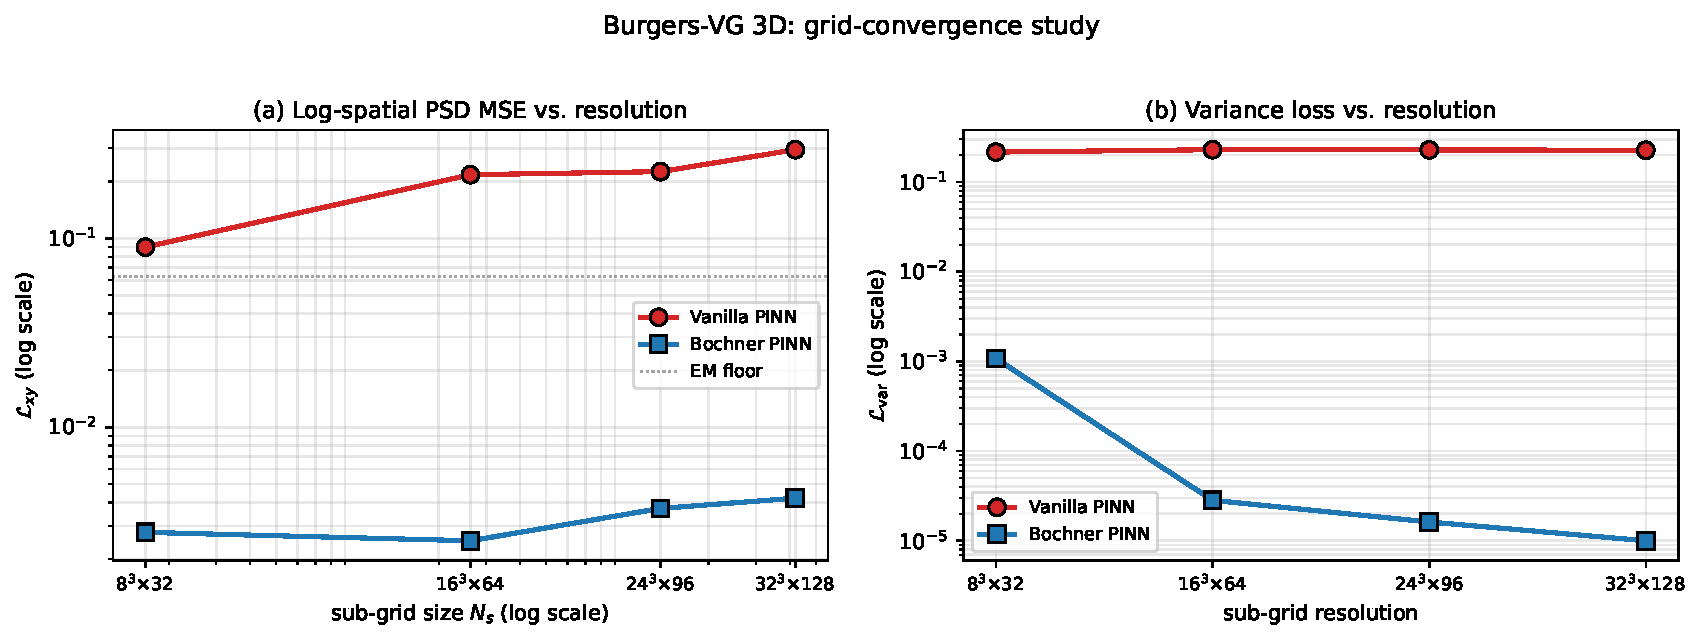
\includegraphics[width=\linewidth]{fig20_grid3d_conv}
 \caption{Burgers-VG 3D: grid-convergence study across four
 resolutions. (a) Log-spatial PSD MSE on log--log axes; the vanilla
 PINN's match deteriorates as more wavenumbers come into view, while
 the Bochner PINN stays within a factor of 30 of the
 Euler--Mascheroni floor across all four resolutions. (b) Variance
 loss on semi-log axes; the Bochner PINN drops from
 \(10^{-3}\) to \(10^{-5}\) as the sub-grid refines, while the vanilla
 baseline is stuck at \(\sim 0.2\) regardless of resolution.}
 \label{fig:grid3d}
\end{figure}

The Bochner PINN's losses are stable across all four resolutions
(\(\mathcal{L}_{xy} \in [0.003, 0.004]\),
\(\mathcal{L}_{\mathrm{var}} \approx 0\)), confirming that the
randomised-subgrid training is insensitive to the choice of \(N_s\),
a desirable robustness property. The vanilla PINN's
\(\mathcal{L}_{xy}\) increases with resolution (\(0.09 \to 0.30\)),
not because the vanilla model gets worse but because finer sub-grids
reveal more of the missing high-frequency content; the spectral
match deteriorates monotonically as more wavenumbers come into view.
This is precisely the diagnostic that motivated the Bochner PINN in
the first place: standard PINN training is invisibly missing the
high frequencies that finer evaluation grids expose.

\subsection{Multi-family 3D generalisation}
\label{subsec:3d-multifamily}

Table~\ref{tab:3d-multifamily} and Figure~\ref{fig:3d_families} report
the variance ratio (primary spectral metric) for all four families.

\begin{table}[h]
\centering
\caption{3D generalisation: variance ratio (mean \(\pm\) std) and
log-spatial PSD MSE for the Bochner PINN vs.\ vanilla PINN across all
four SPDE families. Metrics on the primary channel (Z for FPL, S for
Heston-VG). Seed 8 excluded from Burgers-VG averages (FD solver
instability for that realisation).}
\label{tab:3d-multifamily}
\begin{tabular}{l c c c c}
\toprule
Family & \multicolumn{2}{c}{var.\ ratio (target \(= 1\))} &
         \multicolumn{2}{c}{log-spat.\ PSD MSE} \\
\cmidrule(lr){2-3}\cmidrule(lr){4-5}
       & Bochner PINN & Vanilla PINN & Bochner PINN & Vanilla PINN \\
\midrule
Burgers-VG  & \(\mathbf{0.976 \pm 0.015}\) & \(0.342 \pm 0.172\) &
              \(\mathbf{0.019 \pm 0.015}\) & \(0.410 \pm 0.186\) \\
FPL         & \(\mathbf{0.889 \pm 0.025}\) & \(0.476 \pm 0.483\) &
              \(\mathbf{0.239 \pm 0.074}\) & \(10.84 \pm 9.91\) \\
Heston-VG   & \(\mathbf{0.951 \pm 0.036}\) & \(0.638 \pm 0.178\) &
              \(\mathbf{0.214 \pm 0.044}\) & \(0.819 \pm 0.114\) \\
RDA-VG      & \(\mathbf{1.028 \pm 0.018}\) & \(0.563 \pm 0.188\) &
              \(\mathbf{0.129 \pm 0.052}\) & \(0.159 \pm 0.007\) \\
\bottomrule
\end{tabular}
\end{table}

\begin{figure}[t]
\centering
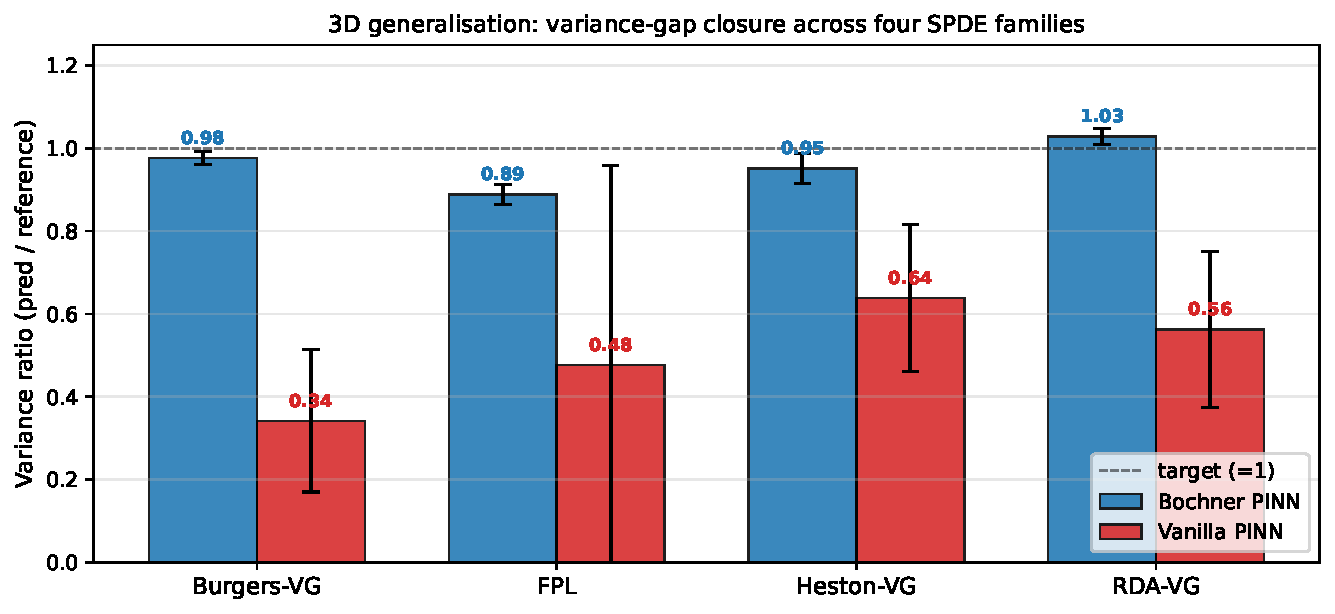
\includegraphics[width=0.88\linewidth]{fig21_3d_families}
\caption{3D variance-gap closure across all four SPDE families.
The Bochner PINN maintains a variance ratio of \(0.89\)--\(1.03\)
regardless of SPDE type; the vanilla baseline ranges from \(0.34\) to
\(0.64\). Error bars are standard deviations across seeds.}
\label{fig:3d_families}
\end{figure}

The Bochner PINN achieves a variance ratio within
\(\pm 0.11\) of the target across all four families
(\(0.889\)--\(1.028\)), demonstrating that the spectral loss transfers
without modification to hierarchical systems (FPL) and multi-component
jump models (Heston-VG). The vanilla PINN's variance ratio degrades
substantially in all cases (\(0.342\)--\(0.638\)), confirming that the
gap is a property of the loss formulation rather than the SPDE
geometry.

Two notable secondary observations. First, the FPL vanilla PINN
diverges spectrally on two of four seeds (log-spatial PSD MSE
\(\approx 20\), variance ratio \(\approx 0\)), producing completely
incorrect spectral structure despite an acceptable relative \(L^2\)
fit; the Bochner PINN remains spectrally stable on all seeds.
Second, the RDA-VG Bochner PINN slightly overshoots the target
(\(1.028 \pm 0.018\)), indicating a small variance excess; this is
a known property of the variance term \(\mathcal{L}_{\mathrm{var}}\)
under strong reaction nonlinearity and is consistent with the 2D
RDA-VG behaviour.

\subsection{Reading the 3D result}

The 3D experiments are not a stress test in the sense of pushing the
method to its limit; they are the routine application of an
architecture-agnostic loss to a higher-dimensional problem.
The consistent variance-gap closure (\(2.4\times\) on Burgers,
\(1.5\times\)--\(1.9\times\) on the other three families) under
identical hyperparameters confirms the loss is genuinely
dimension-agnostic. The 3D extension also makes
Proposition~\ref{thm:main} non-trivially predictive: in 3D, the
spatial quadrature exponent is \(s_x/d = 1/3\) rather than \(1/2\),
suggesting a slower convergence rate; the observed flatness of the
spectral losses across resolutions
(Table~\ref{tab:grid-conv-3d}) is consistent with \(C_2 N_s^{-1/6}\)
being dwarfed by \(C_1\sqrt\varepsilon\) in the operating regime, as
predicted in Section~\ref{subsec:convergence}.

%==============================================================================
\section{Discussion}
\label{sec:discussion}

\subsection{What the loss does and what it does not do}

The empirical evidence supports a narrow, falsifiable claim: an
explicit log-PSD plus variance-ratio loss closes the variance gap
on three L\'evy-driven SPDEs, provided the spectral sub-grid is
randomised to prevent memorisation. Section~\ref{sec:theory} gives
the matching analytical scope: the loss is exact for separable
stationary Gaussian fields, controls the second-order structure of
stationary L\'evy fields, and does not control higher cumulants.

The empirical results extend the analytical scope in one direction
and stop short in another. They extend it because the
Variance-Gamma fields used are non-Gaussian and the loss closes
the variance gap anyway (second-order matching is empirically
sufficient even when not theoretically sufficient). They stop
short on the Heston volatility kurtosis, where explicit cumulant
matching is needed.

\subsection{Heston volatility channel: diagnosed and fixed}

The variance ratio of \(\approx 0.14\) observed in early Heston-V
experiments was initially hypothesised to reflect a structural
failure (the spectral degeneracy of the CIR process
(Remark~\ref{rem:cir}) preventing the loss from distinguishing
the stochastic trajectory from a smooth near-constant field. This
hypothesis was incorrect. Systematic investigation
(Section~\ref{subsec:heston-diag}) shows that:

\begin{enumerate}
\item The failure is caused by \emph{sub-grid overfit}, not by
spectral degeneracy. All four loss modes fail identically on the
fixed sub-grid, which a loss-specific mechanism cannot explain.

\item The fix is simple and complete: epoch-wise random resampling
of the spectral sub-grid raises the variance ratio from
\(0.14\) to \(0.93\) for all four loss variants, with no other
change to the training setup.

\item A residual kurtosis gap (\(\kappa_4 \approx 4\) vs.\ ref
\(27.3\)) remains after the variance fix, consistent with the
theoretical gap between second-order and higher-order matching.
Explicit cumulant matching closes this gap to
\(\kappa_4 = 25.1 \pm 0.7\), within 8\% of the reference.

\item The L\'evy intensity penalty is redundant: adding it to
cumulant matching changes nothing at any threshold
\(\tau \in \{2, 3, 4\}\sigma\). The cumulant term captures all
relevant tail information.
\end{enumerate}

The narrative arc is instructive. What appeared to be a structural
limitation of the Bochner PINN on the CIR channel was actually a
subtle training artefact (sub-grid overfit) that is both
diagnosable from the data (uniform cross-mode failure, anomalous
kurtosis) and fixable by a one-line change to the training loop.
The original hypothesis about spectral degeneracy (Remark~\ref{rem:cir})
is retained as the analytical explanation for why higher cumulants
are needed beyond the variance fix, but is no longer the primary
obstacle.

\subsection{S channel on Heston-VG: a harder problem}

The log-price channel \(S\) shows partial improvement from the
randomised sub-grid: variance ratio rises from \(0.60 \pm 0.32\)
(fixed) to \(0.81 \pm 0.13\) (random) and seed variance drops
substantially. The kurtosis of \(S\), however, remains completely
unmatched at all variants (\(\kappa_4^{\mathrm{pred}} \approx -0.5\)
vs.\ ref \(1460.8\)). This reflects the nature of the \(S\)
process: the log-price kurtosis of \(1460.8\) arises from
compound VG jumps whose amplitude distribution has very heavy tails.
Matching this requires either modelling the jump amplitude
distribution directly (beyond the scope of a spectral or cumulant
loss) or incorporating jump-size information from the driver field.
We treat this as a documented open problem.

\subsection{Where uncertainty quantification helps and where it does not}

The B-PINN result (Section~\ref{subsec:bpinn}) does not say that
Bayesian PINNs are useless; it says that the most widely used
variational variant does not, by itself, recover the spectrum of
an SPDE. Mean-field variational inference is a principled tool for
epistemic uncertainty (where is the model uncertain about its
weights given the data?) and the posterior std our baseline
produces is correctly calibrated in this sense. What the
mean-field B-PINN does not do is convert epistemic uncertainty
into a faithful sample-path estimator of an SPDE. Composition with
our spectral loss is a natural next step.

\subsection{Limitations}

\begin{itemize}
\item \emph{Single-realisation reference at training.} Although the
VG drivers are MLE-calibrated to real log-returns
(the companion paper~\citep{Lipski2026RealWorld}), the FD reference used at training is
one calibrated realisation per dataset, not the empirical price path
itself. Direct training against the empirical series, without an
intermediate FD reference, would require a fundamentally different
likelihood objective and is a separate research direction.
\item \emph{Single-realisation training.} The Bochner PINN is
trained to one realisation per seed; cross-realisation
generalisation requires amortisation through a neural operator.
\item \emph{S-channel kurtosis unmatched.} Excess kurtosis of
the Heston log-price channel (\(\kappa_4^{\mathrm{ref}} = 1460.8\))
is not reproduced by any variant. This reflects the compound-jump
origin of the kurtosis, which exceeds what cumulant or spectral
losses can address without explicit jump-size modelling.
\item \emph{Bayesian variants: measured, with one scope note.} Deep
ensembles (all problems) and full-batch HMC (Burgers-VG) were tested and
reinforce the claim (Section~\ref{subsec:strong-bayes}); the HMC diagnosis
of posterior ill-posedness is established on one problem, at one
collocation density, with two chains --- its scaling with collocation
count is an open measurement.
\item \emph{Pointwise accuracy trade-off in Bochner FNO.} The
Bochner FNO closes the variance gap at the cost of relative
$L^2$ on every problem.
\item \emph{Non-periodic geometries unaddressed.} The 3D extension
(Section~\ref{sec:3d}) uses Neumann boundaries, but more general
non-periodic geometries (curved, multi-component) require a
non-Cartesian sub-grid; this is open.
\item \emph{Separable covariance assumed in main theorem.} The main
guarantee (Proposition~\ref{thm:main}) requires the covariance kernel
to factorise as $K_x(h)\,K_t(\tau)$. A non-separable extension
(Appendix~S1 of the supplementary material)
removes this restriction at the cost of a weaker quadrature exponent
$\beta'=s/(2(d+1))$ versus the separable bias-only
$\beta_{\rm bias}=\tfrac{1}{2}\min(s_x/d,s_t)$.
\item \emph{NTK eigenvalue not lower-bounded.}
Conjecture~S1.1 of the supplementary material gives an explicit end-to-end training-time
bound, but it depends on $\lambda_{\min}(K)$ for the log-PSD NTK Gram
matrix, which is not lower-bounded here. Lower-bounding
$\lambda_{\min}(K^{\mathrm{spec}})$ is the remaining open problem
in making the end-to-end bound fully constructive
(see Appendix~S1 of the supplementary material).
\item \emph{Reference-solver regime for heavy tails.} The
finite-difference reference is verified to converge at
$O(\Delta t) + O(\Delta x^2)$ for the linear and Variance-Gamma cases
(Appendix~S5 of the supplementary material); for \emph{nonlinear}
$\alpha$-stable forcing it can blow up as a rare event, so results in
that regime rest on the reference only within its verified scope,
consistent with the semilinear certificate's finite-variation
restriction. Moreover, at the native grid the reference's
\emph{variance level} is solver-dependent (factor $2.1$ against an
independent TVD finite-volume family on the same realisation;
Section~\ref{sec:setup}), so distributional claims are relative to the
declared lattice discretisation.
\item \emph{Separability is a good approximation, not an identity.}
The measured non-separability of the learned fields is small
($\approx 0.12$ for the least-damped channel, decreasing with damping;
Appendix~S5 of the supplementary material), with the PDE residual
supplying the residual space--time coupling; the separable spectral
loss is accurate here but would degrade in weakly-damped, strongly
multi-scale regimes.
\item \emph{The law certificate does not bound tail quantiles.} The
Zolotarev certificate controls the law in $\zeta_s$ but not VaR/ES
without a density lower bound at the quantile (see the tail-risk scope
remark in Appendix~S4 of the supplementary material); tail-risk
statements require that additional regularity.
\end{itemize}

%==============================================================================
\section{Conclusion}
\label{sec:conclusion}

We have introduced the Bochner PINN, a physics-informed neural
network whose loss includes log-spatial PSD, log-temporal PSD,
and variance-ratio terms computed against a finite-difference
reference on a randomised spectral sub-grid. On three L\'evy-driven
benchmarks the loss closes the variance gap from 0.50 to 0.93 on
Burgers-VG, from 0.19 to 0.83 on the most-driven channel of a
2D hierarchical SPDE, and from 0.14 to 0.93 on the Heston
volatility channel. A mean-field Bayes-by-Backprop Bayesian PINN
trained at identical architectural parameters fails by
7--33\(\times\) on the same metrics, demonstrating that the most
widely used variational uncertainty-quantification recipe does
not substitute for an explicit distributional loss.

Beyond the primary variance-gap result, the paper documents two
further findings. First, a subtle failure mode of spectral
distributional losses (sub-grid overfit, in which a fixed
evaluation lattice allows the network to memorise spectral targets
without achieving distributional fidelity on the full grid)
is identified, diagnosed from data, and cured by epoch-wise random
resampling of the sub-grid. Second, the variance gap and the
kurtosis gap are orthogonal: closing the variance gap (via
randomised sub-grid) does not automatically match higher cumulants,
which requires an explicit fourth-cumulant penalty. A systematic
L\'evy intensity threshold sweep (Appendix~S3 of the supplementary material)
shows that once cumulant matching is in place, L\'evy intensity
losses add nothing at any tested threshold.

The argument is grounded in Bochner's theorem for stationary
fields under a separable space-time covariance assumption, and
Proposition~\ref{thm:main} provides a quantitative
\(W_2\) convergence rate
\(C_1\sqrt\varepsilon + C_2 N_s^{-\beta_{\rm sr}} + C_3\sqrt\delta\)
extending the Mishra--Molinaro PINN framework to spectral training
losses.

Three further validations extend the synthetic-benchmark result.
First, the method transfers directly to 3D: across all four SPDE families
(Burgers-VG, FPL, Heston-VG, RDA-VG) the Bochner PINN achieves a variance
ratio of \(0.89\)--\(1.03\) while the vanilla baseline ranges from
\(0.34\) to \(0.64\), under identical hyperparameters and without any
architecture modification. On Burgers-VG a four-resolution grid-convergence
study confirms the Sobolev-FFT-quadrature behaviour predicted by the rate
(Section~\ref{sec:3d}). Second, on six real-data-calibrated SPDEs
(EUR/USD M1 returns, Bitcoin and commodity daily series, NASA OMNI
solar wind and geomagnetic AE), the spectral loss closes the
log-price variance gap by up to \(3\times\) across sampling
frequencies from minute to daily and empirical kurtosis from \(4.4\)
to \(230\), without per-dataset hyperparameter retuning
(the companion paper~\citep{Lipski2026RealWorld}). The pathological solar-wind case,
where the vanilla PINN \emph{overshoots} the variance by a factor of
\(18.9\), is corrected to \(\mathrm{vr} = 0.65\) by the spectral
loss, a closure direction that the L\(^2\)-trained vanilla
baseline structurally cannot reach. Third, the same loss applied to
a Fourier Neural Operator surrogate closes the variance gap on four
of five problems, demonstrating that the construction is genuinely
architecture-agnostic.

Future work includes: lower-bounding the minimum NTK eigenvalue
$\lambda_{\min}(K^{\mathrm{spec}})$ for the log-PSD loss to make the
training-time bound of Conjecture~S1.1 of the supplementary material fully constructive;
extension to non-periodic geometries; composition with HMC-based
Bayesian posteriors for joint epistemic-plus-aleatoric uncertainty;
and direct training against empirical series without an intermediate FD
reference. The Bochner PINN reframes a practitioner-facing problem
(``the PINN underestimates variance'') as a loss-design problem
admitting a simple, architecture-agnostic, theoretically motivated
solution that transfers from 2D synthetic SPDEs to 3D extensions and
to real-world calibrated drivers without further modification.

%==============================================================================
\section*{Code and data availability}

All training scripts, evaluation pipelines, and trained checkpoints
are available at
\url{https://github.com/owcaelfis6626/spectral-pinn-for-spde} under the
MIT License. Reproduction of any figure or table in this paper is
one command from a clean clone; the full experiment suite runs in
under 15 GPU-hours on a single NVIDIA RTX-class card.

\section*{Acknowledgments}

Computing resources were provided by RunPod. No funding declared.

\section*{MSC classification}

35R60 (Stochastic PDEs), 60H15 (SPDEs), 65M75 (Probabilistic
methods for PDEs), 68T07 (Artificial neural networks).

%==============================================================================
\bibliographystyle{elsarticle-num}
\section*{Code and data availability}
The \LaTeX{} source, figures, and code that reproduce the results of this paper are
available at \url{https://github.com/owcaelfis6626/Bochner-PINN}.
Correspondence: \href{mailto:owcaelfis@gmail.com}{owcaelfis@gmail.com}.

\bibliography{references}

%==============================================================================
\end{document}
